% !TEX root = ../Elements.tex
%%%%%%
% BOOK 9
%%%%%%
\pdfbookmark[0]{Book 9}{book9}
\pagestyle{empty}
\begin{center}
{\Huge ELEMENTS BOOK 9}\\
\spa\spa\spa
{\huge\it Applications of Number Theory\symbolfootnote[2]{The propositions contained in Books 7--9 are generally attributed to the
school of Pythagoras.}}
\end{center}
%\vspace{2cm}
%% Removed epsf size command
%\centerline{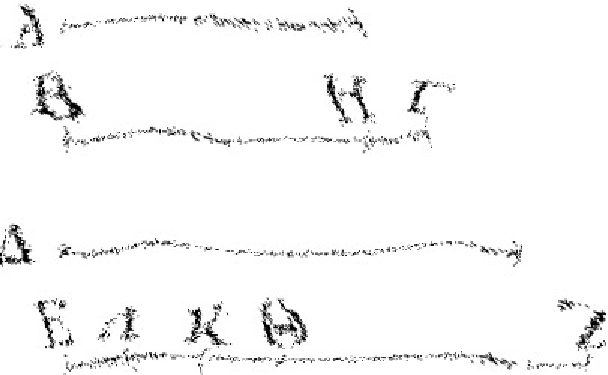
\includegraphics{Book09/front.pdf}}
\newpage

%%%%%%
% Prop 9.1
%%%%%%
\pdfbookmark[1]{Proposition 9.1}{pdf9.1}
\pagestyle{fancy}
\cfoot{\gr{\kern -.7pt }}
\lhead{\large\gr{ΣΤΟΙΘΕΙΩΝ \kern -.7pt {9}.}}
\rhead{\large ELEMENTS BOOK 9}
\begin{Parallel}{}{} 
\ParallelLText{
\begin{center}
{\large \ggn{1}.}
\end{center}\vspace*{-7pt}

\gr{Ἐὰν δύο <όμοιοι ἐπίπεδοι ἀριθμοὶ πολλαπλασιάσαντεξ ἀλλήλουξ
ποιῶσί τινα, ὁ γενόμενοξ τετράγωνοξ >έσται.}\\

% Removed epsf size command
\centerline{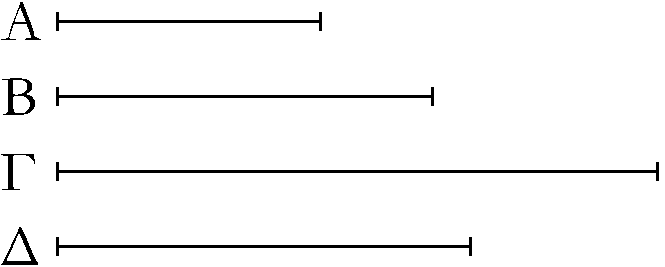
\includegraphics{Book09/fig01g.pdf}}

\gr{>'Εστωσαν δύο <όμοιοι ἐπίπεδοι ἀριθμοὶ οἱ Α, Β, καὶ ὁ Α τὸν
Β πολλαπλασιάσαξ τὸν Γ ποιείτω; λέγω, <ότι ὁ Γ τετράγωνόξ ἐστιν.}

\gr{Ὁ γὰρ Α ἑαυτὸν πολλαπλασιάσαξ τὸν Δ ποιείτω. ὁ Δ >άρα τετράγωνόξ ἐστιν. ἐπεὶ ο>ῦν ὁ Α ἑαυτὸν μὲν πολλαπλασιάσαξ τὸν Δ πεποίηκεν, τὸν δὲ Β πολλαπλασιάσαξ τὸν Γ πεποίηκεν, >έστιν >άρα
ὡξ ὁ Α πρὸξ τὸν Β, ο<ύτωξ ὁ Δ πρὸξ τὸν Γ. καὶ ἐπεὶ
οἱ Α, Β <όμοιοι ἐπίπεδοί εἰσιν ἀριθμοί, τῶν Α, Β >άρα ε<ῖξ
μέσοξ ἀνάλογον ἐμπίπτει ἀριθμόξ. ἒαν δὲ δύο ἀριθμῶν
μεταχὺ κατὰ τὸ συνεθὲξ ἀνάλογον ἐμπίπτωσιν ἀριθμοί, <όσοι
εἰξ α\kern -.7pt  ὐτοὺξ ἐμπίπτουσι, τοσοῦτοι καὶ εἰξ τοὺξ τὸν α\kern -.7pt  ὐτὸν
λόγον >έθονταξ; <ώστε καὶ τῶν Δ, Γ ε<ῖξ μέσοξ ἀνάλογον
ἐμπίπτει ἀριθμόξ. καί ἐστι τετράγωνοξ ὁ Δ; τετράγωνοξ
>άρα καὶ ὁ Γ; <όπερ >έδει δεῖχαι.}}

\ParallelRText{
\begin{center}
{\large Proposition 1}
\end{center}

If two similar plane numbers make some (number by) multiplying one another then the created (number) will be  square.\\

% Removed epsf size command
\centerline{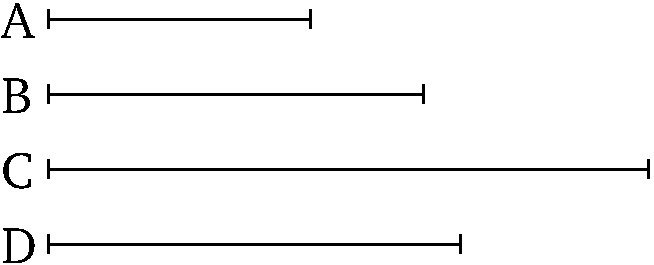
\includegraphics{Book09/fig01e.pdf}}

Let $A$ and $B$ be two similar plane numbers, and let $A$ make $C$
(by) multiplying $B$. I say that $C$ is square.

For let $A$ make $D$ (by) multiplying itself. $D$ is thus square. Therefore, since $A$ has made $D$ (by) multiplying itself, and
has made $C$ (by) multiplying $B$, thus as $A$ is to $B$, so $D$ (is) to $C$ [Prop.~7.17]. And since $A$ and $B$ are similar
plane numbers, one number thus falls (between) $A$ and $B$ in mean
proportion [Prop.~8.18]. And if (some) numbers fall between two  numbers in continued proportion then, as many (numbers)
as fall in  (between) them (in continued proportion), so many also (fall) in (between numbers) having
the same ratio (as them in continued proportion)  [Prop.~8.8].
And hence one number falls (between) $D$ and $C$ in mean proportion.
And $D$ is  square. Thus, $C$ (is) also  square [Prop.~8.22]. (Which is)
the very thing it was required to show.}
\end{Parallel}

%%%%%%
% Prop 9.2
%%%%%%
\pdfbookmark[1]{Proposition 9.2}{pdf9.2}
\begin{Parallel}{}{} 
\ParallelLText{
\begin{center}
{\large \ggn{2}.}
\end{center}\vspace*{-7pt}

\gr{Ἐὰν δύο ἀριθμοὶ πολλαπλασιάσαντεξ ἀλλήλουξ ποιῶσι τετράγωνον,
<όμοιοι ἐπίπεδοί εἰσιν ἀριθμοί.}

% Removed epsf size command
\centerline{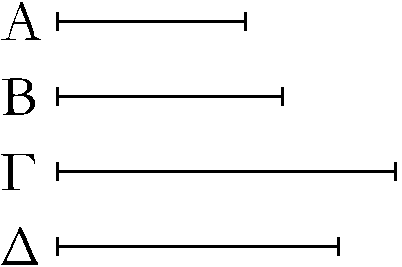
\includegraphics{Book09/fig02g.pdf}}

\gr{>'Εστωσαν δύο ἀριθμοὶ οἱ Α, Β, καὶ ὁ Α τὸν Β πολλαπλασιάσαξ
τετράγωνον τὸν Γ ποιείτω; λέγω, <ότι οἱ Α, Β <όμοιοι
ἐπίπεδοί εἰσιν ἀριθμοί.}

\gr{Ὁ γὰρ Α ἑαυτὸν πολλαπλασιάσαξ τὸν Δ ποιείτω; ὁ Δ >άρα
τετράγωνόξ ἐστιν. καὶ ἐπεὶ ὁ Α ἑαυτὸν μὲν πολλαπλασιάσαξ τὸν
Δ πεποίηκεν, τὸν δὲ Β πολλαπλασιάσαξ τὸν Γ πεποίηκεν, >έστιν
>άρα ὡξ ὁ Α πρὸξ  τὸν Β, ὁ Δ πρὸξ τὸν Γ. καὶ ἐπεὶ ὁ Δ
τετράγωνόξ ἐστιν, ἀλλὰ καὶ ὁ Γ, οἱ Δ, Γ >άρα <όμοιοι
ἐπίπεδοί εἰσιν.
 τῶν Δ, Γ >άρα ε<ῖξ μέσοξ ἀνάλογον
ἐμπίπτει. καί ἐστιν ὡξ ὁ Δ πρὸξ τὸν Γ, ο<ύτωξ ὁ Α πρὸξ τὸν
Β; καὶ τῶν Α, Β >άρα ε~ἱξ μέσοξ ἀνάλογον ἐμπίπτει.
ἒαν δὲ δύο ἀριθμῶν ε<ῖξ μέσοξ ἀνάλογον ἐμπίπτῃ,
<όμοιοι ἐπίπεδοί εἰσιν [οἱ] ἀριθμοί; οἱ >άρα Α, Β <όμοιοί
εἰσιν ἐπίπεδοι; <όπερ >έδει δεῖχαι.}}

\ParallelRText{
\begin{center}
{\large Proposition 2}
\end{center}

If two numbers make a square (number by)
multiplying one another then they are similar plane numbers.

% Removed epsf size command
\centerline{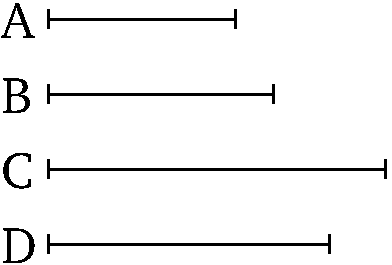
\includegraphics{Book09/fig02e.pdf}}

Let $A$ and $B$ be two numbers, and let $A$ make the square (number)
$C$ (by) multiplying $B$. I say that $A$ and $B$ are similar plane numbers.

For let $A$ make $D$ (by) multiplying itself. Thus, $D$ is square. And since $A$ has made $D$ (by) multiplying itself, and has made $C$ (by)
multiplying $B$, thus as $A$ is to $B$, so $D$ (is) to $C$ [Prop.~7.17]. And since $D$ is  square, and $C$ (is) also, $D$ and $C$ are thus similar plane numbers. Thus, 
one (number) falls (between) $D$ and $C$ in mean proportion [Prop.~8.18]. And as $D$ is to $C$, so $A$ (is) to $B$. Thus, one (number) also falls (between) $A$ and $B$ in mean proportion [Prop.~8.8].  And if one (number)
falls (between) two numbers in mean proportion then [the] numbers
are similar plane (numbers)  [Prop.~8.20].
Thus, $A$ and $B$ are similar plane (numbers). (Which is) the
very thing it was required to show.}
\end{Parallel}

%%%%%%
% Prop 9.3
%%%%%%
\pdfbookmark[1]{Proposition 9.3}{pdf9.3}
\begin{Parallel}{}{} 
\ParallelLText{
\begin{center}
{\large \ggn{3}.}
\end{center}\vspace*{-7pt}

\gr{Ἐὰν κύβοξ ἀριθμὸξ ἑαυτὸν πολλαπλασιάσαξ ποιῆ| τινα, ὁ γενόμενοξ
κύβοξ >έσται.}

% Removed epsf size command
\centerline{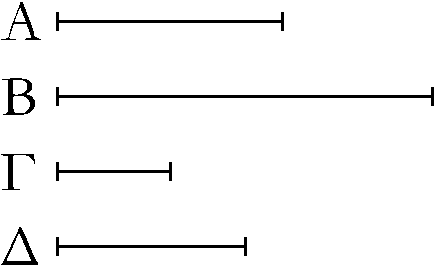
\includegraphics{Book09/fig03g.pdf}}

\gr{Κύβοξ γὰρ ἀριθμὸξ ὁ Α ἑαυτὸν πολλαπλασιάσαξ τὸν Β ποιείτω;
λέγω, <ότι ὁ Β κύβοξ ἐστίν.}

\gr{Εἰλήφθω γὰρ τοῦ Α πλευρὰ ὁ Γ, καὶ ὁ Γ ἑαυτὸν πολλαπλασιάσαξ τὸν
Δ ποιείτω. φανερὸν δή ἐστιν, <ότι ὁ Γ τὸν Δ πολλαπλασιάσαξ
τὸν Α πεποίηκεν. καὶ ἐπεὶ ὁ Γ ἑαυτὸν πολλαπλασιάσαξ τὸν Δ
πεποίηκεν, ὁ Γ >άρα τὸν Δ μετρεῖ κατὰ τὰξ ἐν α\kern -.7pt  ὐτῶ| μονάδαξ.
ἀλλὰ μ\kern -.7pt  ὴν καὶ ἡ μονὰξ τὸν Γ μετρεῖ κατὰ τὰξ ἐν α\kern -.5pt  ὐτῶ|
μονάδαξ; >έστιν >άρα ὡξ ἡ μονὰξ πρὸξ τὸν Γ, ὁ Γ πρὸξ
τὸν Δ. πάλιν, ἐπεὶ ὁ Γ τὸν Δ πολλαπλασιάσαξ τὸν Α πεποίηκεν,
ὁ Δ >άρα τὸν Α μετρεῖ κατὰ τὰξ ἐν τῶ| Γ μονάδαξ. μετρεῖ δὲ καὶ ἡ
μονὰξ τὸν Γ κατὰ τὰξ ἐν α\kern -.3pt  ὐτῶ| μονάδαξ; >έστιν >άρα ὡξ ἡ μονὰξ
πρὸξ τὸν Γ, ὁ Δ πρὸξ τὸν Α. ἀλλ> ὡξ ἡ μονὰξ πρὸξ τὸν Γ,
ὁ Γ πρὸξ τὸν Δ; καὶ ὡξ >άρα ἡ μονὰξ πρὸξ τὸν Γ, ο<ύτωξ
ὁ Γ πρὸξ τὸν Δ καὶ ὁ Δ πρὸξ τὸν Α. τῆξ >άρα μονάδοξ
καὶ τοῦ Α ἀριθμοῦ δύο μέσοι ἀνάλογον
κατὰ τὸ συνεθὲξ ἐμπεπτώκασιν ἀριθμοὶ οἱ Γ, Δ.
πάλιν, ἐπεὶ ὁ Α ἑαυτὸν πολλαπλασιάσαξ τὸν Β πεποίηκεν, ὁ Α
>άρα τὸν Β μετρεῖ κατὰ τὰξ ἐν α\kern -.7pt  ὐτῶ| μονάδαξ;
μετρεῖ δὲ καὶ ἡ μονὰξ τὸν Α κατὰ τὰξ ἐν α\kern -.7pt  ὐτῶ|
μονάδαξ;
 >έστιν
>άρα ὡξ ἡ μονὰξ πρὸξ τὸν Α, ὁ Α πρὸξ τὸν Β. τῆξ δὲ μονάδοξ
καὶ τοῦ Α δύο μέσοι ἀνάλογον ἐμπεπτώκασιν ἀριθμοί; καὶ
τῶν Α, Β >άρα δύο μέσοι ἀνάλογον ἐμπεσοῦνται ἀριθμοί. ἒαν
δὲ δύο ἀριθμῶν δύο μέσοι ἀνάλογον ἐμπίπτωσιν, ὁ δὲ
πρῶτοξ κύβοξ >ῆ|, καὶ ὁ δεύτεροξ κύβοξ >έσται. καί ἐστιν
ὁ Α κύβοξ; καὶ ὁ Β >άρα κύβοξ ἐστίν; <όπερ >έδει
δεῖχαι.}}

\ParallelRText{
\begin{center}
{\large Proposition 3}
\end{center}

If a cube number makes some (number by) multiplying itself then the created (number) will be cube.

% Removed epsf size command
\centerline{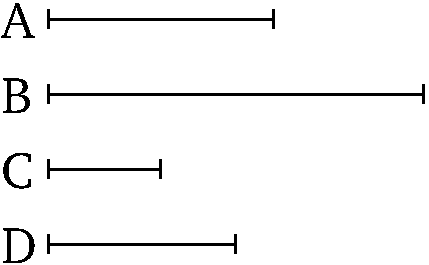
\includegraphics{Book09/fig03e.pdf}}

For let the cube number $A$ make $B$ (by) multiplying itself. I say
that $B$ is  cube.

For let the side $C$ of $A$ be taken. And let $C$ make
$D$ by multiplying itself. So it is clear that $C$ has made $A$ (by)
multiplying $D$. And since $C$ has made $D$ (by) multiplying itself,
$C$ thus measures $D$ according to the units in it [Def.~7.15]. But, in fact, a unit also measures
$C$ according to the units in it [Def.~7.20]. 
Thus, as a unit is to $C$, so $C$ (is) to $D$. Again, since $C$ has
made $A$ (by) multiplying $D$, $D$ thus measures $A$ according to
the units in $C$. And a unit also measures $C$ according to the units in it. Thus, as a unit is to $C$, so $D$ (is) to $A$. But, as a unit (is) to $C$, so
$C$ (is) to $D$. And thus as a unit (is) to $C$, so $C$ (is) to $D$, and
$D$ to $A$. Thus, two numbers, $C$ and $D$, have fallen (between) a unit
and the number $A$ in continued  mean proportion. Again, since $A$ has made $B$ (by) multiplying itself, $A$ thus measures $B$ according to the units in it.
And a unit also measures $A$ according to the units in it. Thus, as a
unit is to $A$, so $A$ (is) to $B$. And two numbers have
fallen (between) a unit and $A$ in mean proportion. Thus two
numbers will also fall (between) $A$ and $B$ in mean proportion [Prop.~8.8].
And if two
(numbers) fall (between) two numbers in mean proportion, and the
first (number) is cube, then the second will also be  cube 
[Prop.~8.23]. And $A$ is cube.
Thus, $B$ is also  cube. (Which is) the very thing it was required to show.}
\end{Parallel}

%%%%%%
% Prop 9.4
%%%%%%
\pdfbookmark[1]{Proposition 9.4}{pdf9.4}
\begin{Parallel}{}{} 
\ParallelLText{
\begin{center}
{\large \ggn{4}.}
\end{center}\vspace*{-7pt}

\gr{Ἐὰν κύβοξ ἀριθμὸξ κύβον ἀριθμὸν πολλαπλασιάσαξ ποιῆ| τινα,
ὁ γενόμενοξ κύβοξ >έσται.}

\gr{Κύβοξ γὰρ ἀριθμὸξ ὁ Α κύβον ἀριθμὸν τὸν Β πολλαπλασιάσαξ
τὸν Γ ποιείτω; λέγω, <ότι ὁ Γ κύβοξ ἐστίν.}

% Removed epsf size command
\centerline{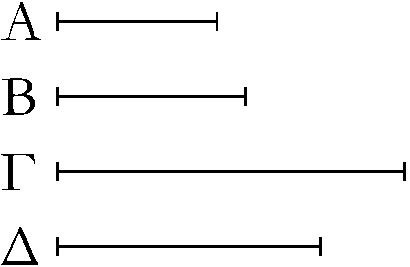
\includegraphics{Book09/fig04g.pdf}}

\gr{Ὁ γὰρ Α ἑαυτὸν πολλαπλασιάσαξ τὸν Δ ποιείτω;
ὁ Δ >άρα κύβοξ ἐστίν. καὶ ἐπεὶ ὁ Α ἑαυτὸν μὲν
πολλαπλασιάσαξ τὸν Δ πεποίηκεν, τὸν δὲ Β πολλαπλασιάσαξ τὸν Γ
πεποίηκεν,  >έστιν >άρα ὡξ ὁ Α πρὸξ τὸν Β, ο<ύτωξ ὁ Δ πρὸξ
τὸν Γ. καὶ ἐπεὶ οἱ Α, Β κύβοι εἰσίν, <όμοιοι στερεοί εἰσιν οἱ Α, Β.
τῶν Α, Β >άρα δύο μέσοι ἀνάλογον ἐμπίπτουσιν ἀριθμοί;
<ώστε καὶ τῶν Δ, Γ δύο μέσοι ἀνάλογον ἐμπεσοῦνται ἀριθμοί.
καί ἐστι κύβοξ ὁ Δ; κύβοξ >άρα καὶ ὁ Γ; <όπερ >έδει δεῖχαι.}}

\ParallelRText{
\begin{center}
{\large Proposition 4}
\end{center}

If a cube number makes some (number by) multiplying a(nother) cube number then the created (number) will be  cube.

For let the cube number $A$ make $C$ (by) multiplying the cube number $B$. I say that $C$ is cube.

% Removed epsf size command
\centerline{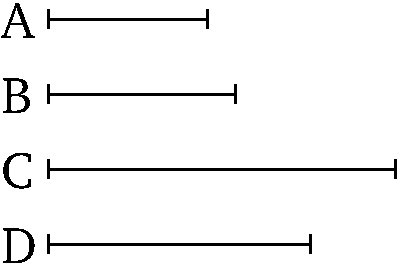
\includegraphics{Book09/fig04e.pdf}}

For let $A$ make $D$ (by) multiplying itself.  Thus, $D$ is  cube 
[Prop.~9.3]. And since $A$ has made
$D$ (by) multiplying itself, and has made $C$ (by) multiplying $B$, 
thus as $A$ is to $B$, so $D$ (is) to $C$ [Prop.~7.17].  And since $A$ and $B$ are cube, $A$ and $B$ are similar solid (numbers). Thus, two numbers fall
(between) $A$ and $B$ in mean proportion [Prop.~8.19]. Hence, two numbers will
also fall (between) $D$ and $C$ in mean proportion [Prop.~8.8]. And $D$ is  cube. Thus,
$C$ (is) also cube  [Prop.~8.23]. 
(Which is) the very thing it was required to show.}
\end{Parallel}

%%%%%%
% Prop 9.5
%%%%%%
\pdfbookmark[1]{Proposition 9.5}{pdf9.5}
\begin{Parallel}{}{} 
\ParallelLText{
\begin{center}
{\large \ggn{5}.}
\end{center}\vspace*{-7pt}

\gr{Ἐὰν κύβοξ ἀριθμὸξ ἀριθμόν τινα πολλαπλασιάσαξ κύβον ποιῆ|,
καὶ ὁ πολλαπλασιασθεὶξ κύβοξ >έσται.}\\

% Removed epsf size command
\centerline{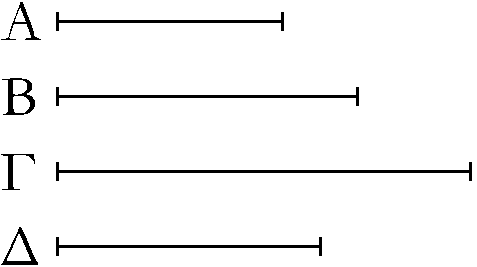
\includegraphics{Book09/fig05g.pdf}}

\gr{Κύβοξ γὰρ ἀριθμὸξ ὁ Α ἀριθμόν τινα τὸν Β πολλαπλασιάσαξ κύβον
τὸν Γ ποιείτω; λέγω, <ότι ὁ Β κύβοξ ἐστίν.}

\gr{Ὁ γὰρ Α ἑαυτὸν πολλαπλασιάσαξ τὸν Δ ποιείτω; κύβοξ >άρα ἐστίν
ὁ Δ. καὶ ἐπεὶ ὁ Α ἑαυτὸν μὲν πολλαπλασιάσαξ τὸν Δ πεποίηκεν, τὸν
δὲ Β πολλαπλασιάσαξ τὸν Γ πεποίηκεν, >έστιν ἀρα ὡξ ὁ Α πρὸξ τὸν Β,
ὁ Δ πρὸξ τὸν Γ. καὶ ἐπεὶ οἱ Δ, Γ κύβοι εἰσίν, <όμοιοι στερεοί
εἰσιν. τῶν Δ, Γ >άρα δύο μέσοι ἀνάλογον ἐμπίπτουσιν ἀριθμοί.
καί ἐστιν ὡξ ὁ Δ πρὸξ τὸν Γ, ο<ύτωξ ὁ Α πρὸξ τὸν Β; καὶ τῶν
Α, Β >άρα δύο μέσοι ἀνάλογον ἐμπίπτουσιν ἀριθμοί. καί ἐστι
κύβοξ ὁ Α; κύβοξ >άρα ἐστὶ καὶ ὁ Β; <όπερ >έδει δεῖχαι.}}

\ParallelRText{
\begin{center}
{\large Proposition 5}
\end{center}

If a cube number makes a(nother) cube number
(by) multiplying some (number) then the (number) multiplied will also be 
cube.

% Removed epsf size command
\centerline{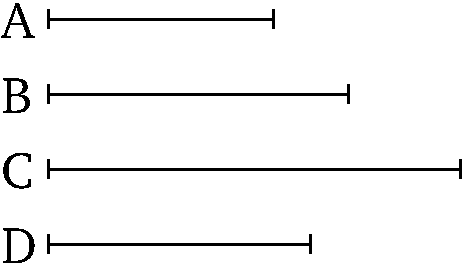
\includegraphics{Book09/fig05e.pdf}}

For let the cube number $A$ make the cube (number) $C$ (by) multiplying
some number $B$. I say that $B$ is cube.

For let $A$ make $D$ (by) multiplying itself. $D$ is thus  cube [Prop.~9.3]. And since $A$ has made $D$ (by)
multiplying itself, and has made $C$ (by) multiplying $B$, thus as $A$ is to
$B$, so $D$ (is) to $C$ [Prop.~7.17]. And since
$D$ and $C$ are (both) cube, they are similar solid (numbers). Thus,
two numbers fall (between) $D$ and $C$ in mean proportion [Prop.~8.19]. And as $D$  is to $C$, so $A$ (is) to $B$.  Thus, two numbers also fall (between) $A$ and $B$ in mean proportion
[Prop.~8.8]. And $A$ is  cube. Thus,
 $B$ is also  cube  [Prop.~8.23]. (Which is) the very thing it was required to show.}
\end{Parallel}

%%%%%%
% Prop 9.6
%%%%%%
\pdfbookmark[1]{Proposition 9.6}{pdf9.6}
\begin{Parallel}{}{} 
\ParallelLText{
\begin{center}
{\large \ggn{6}.}
\end{center}\vspace*{-7pt}

\gr{Ἐὰν ἀριθμὸξ ἑαυτὸν πολλαπλασιάσαξ κύβον ποιῆ|, καὶ α\kern -.7pt  ὐτὸξ κύβοξ
>έσται.}

\gr{Ἀριθμὸξ γὰρ ὁ Α ἑαυτὸν πολλαπλασιάσαξ κύβον τὸν Β ποιείτω;
λέγω, <ότι καὶ ὁ Α κύβοξ ἐστίν.}

% Removed epsf size command
\centerline{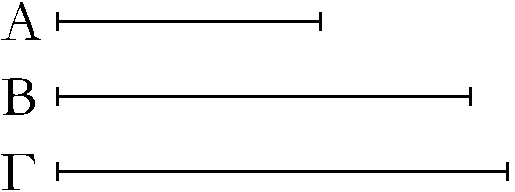
\includegraphics{Book09/fig06g.pdf}}

\gr{Ὁ γὰρ Α τὸν Β πολλαπλασιάσαξ τὸν Γ ποιείτω. ἐπεὶ ο>ῦν ὁ Α
ἑαυτὸν μὲν πολλαπλασιάσαξ τὸν Β πεποίηκεν, τὸν δὲ Β πολλαπλασιάσαξ
τὸν Γ πεποίηκεν, ὁ Γ >άρα κύβοξ ἐστίν. καὶ ἐπεὶ ὁ Α ἑαυτὸν
πολλαπλασιάσαξ τὸν Β πεποίηκεν, ὁ Α >άρα τὸν Β μετρεῖ κατὰ τὰξ
ἐν α\kern -.7pt  ὐτῶ| μονάδαξ. μετρεῖ δὲ καὶ ἡ μονὰξ τὸν Α κατὰ τὰξ
ἐν α\kern -.7pt  ὐτῶ| μονάδαξ. >έστιν >άρα ὡξ ἡ μονὰξ πρὸξ τὸν Α, ο<ύτωξ
ὁ Α πρὸξ τὸν Β. καὶ ἐπεὶ ὁ Α τὸν Β πολλαπλασιάσαξ τὸν Γ πεποίηκεν,
ὁ Β >άρα τὸν Γ μετρεῖ κατὰ τὰξ ἐν τῶ| Α μονάδαξ. μετρεῖ δὲ
καὶ ἡ μονὰξ  τὸν Α κατὰ τὰξ ἐν α\kern -.5pt  ὐτῶ| μονάδαξ. >έστιν >άρα  ὡξ ἡ μονὰξ πρὸξ τὸν Α,
ο<ύτωξ ὁ Β πρὸξ
τὸν Γ. ἀλλ> ὡξ ἡ μονὰξ πρὸξ τὸν Α, ο<ύτωξ ὁ Α πρὸξ τὸν Β;
καὶ ὡξ >άρα ὁ Α πρὸξ τὸν Β, ὁ Β πρὸξ τὸν Γ. καὶ ἐπεὶ οἱ Β, Γ
κύβοι εἰσίν, <όμοιοι στερεοί εἰσιν. τῶν Β, Γ >άρα δύο μέσοι ἀνάλογόν εἰσιν ἀριθμοί. καί ἐστιν ὡξ ὁ Β πρὸξ τὸν Γ, ὁ Α πρὸξ
τὸν Β. καὶ τῶν Α, Β >άρα δύο μέσοι ἀνάλογόν εἰσιν ἀριθμοί.
καί ἐστιν κύβοξ ὁ Β; κύβοξ >άρα ἐστὶ καὶ ὁ Α; <όπερ >έδει
δεῖχαι.}}

\ParallelRText{
\begin{center}
{\large Proposition 6}
\end{center}

If a number makes a cube (number by) multiplying itself then it itself will also be  cube.

For let the number $A$ make the cube (number) $B$ (by) multiplying itself.
I say that $A$ is also cube.

% Removed epsf size command
\centerline{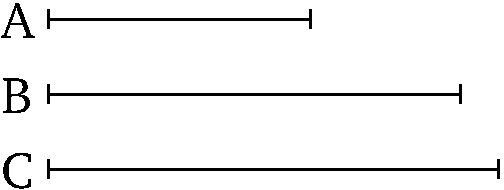
\includegraphics{Book09/fig06e.pdf}}

For let $A$ make $C$ (by) multiplying $B$. Therefore, since $A$
has made $B$ (by) multiplying itself, and has made $C$ (by) multiplying 
$B$, $C$ is thus cube. And since $A$ has made $B$ (by)
multiplying itself, $A$ thus measures $B$ according to the units in ($A$).
And a unit also measures $A$ according to the units in it. Thus, as
a unit is to $A$, so $A$ (is) to $B$. And since $A$ has made $C$ (by)
multiplying $B$, $B$ thus measures $C$ according to the units in $A$.
And a unit also measures $A$ according to the units in it. Thus, as
a unit is to $A$, so $B$ (is) to $C$. But, as a unit (is) to $A$, so $A$ (is)
to $B$. And thus as $A$ (is) to $B$, (so) $B$ (is) to $C$. And since $B$
and $C$ are cube, they are similar solid (numbers). Thus,
there exist two numbers in mean proportion (between) $B$ and $C$ [Prop.~8.19]. And as $B$ is to $C$, (so) $A$ (is)
to $B$. Thus, there also exist two numbers in mean proportion (between) $A$ and
$B$ [Prop.~8.8].  And $B$ is  cube. Thus, $A$
is also  cube   [Prop.~8.23]. (Which is)
the very thing it was required to show.}
\end{Parallel}

%%%%%%
% Prop 9.7
%%%%%%
\pdfbookmark[1]{Proposition 9.7}{pdf9.7}
\begin{Parallel}{}{} 
\ParallelLText{
\begin{center}
{\large \ggn{7}.}
\end{center}\vspace*{-7pt}

\gr{Ἐὰν σύνθετοξ ἀριθμὸξ ἀριθμόν τινα πολλαπλασιά\-σαξ ποιῆ| τινα, ὁ
γενόμενοξ στερεὸξ >έσται.}\\

% Removed epsf size command
\centerline{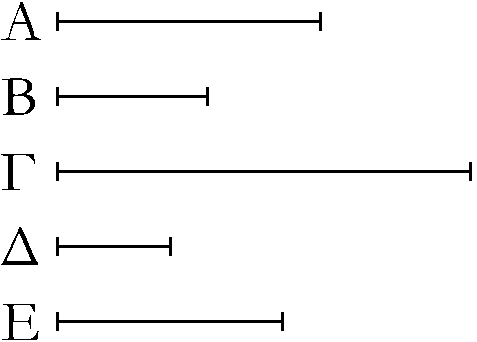
\includegraphics{Book09/fig07g.pdf}}

\gr{Σύνθετοξ γὰρ ἀριθμὸξ ὁ Α ἀριθμόν τινα τὸν Β πολλαπλασιάσαξ 
τὸν Γ ποιείτω; λέγω, <ότι ὁ Γ στερεόξ ἐστιν.}

\gr{Ἐπεὶ γὰρ ὁ Α σύνθετόξ ἐστιν, ὑπὸ ἀριθμοῦ τινοξ μετρηθήσεται.
μετρείσθω ὑπὸ τοῦ Δ, καὶ ὁσάκιξ ὁ Δ τὸν Α μετρεῖ, τοσα\kern -.7pt  ῦται
μονάδεξ >έστωσαν ἐν τῶ| Ε. ἐπεὶ ο>ῦν ὁ Δ τὸν Α μετρεῖ
κατὰ τὰξ ἐν τῶ| Ε μονάδαξ, ὁ Ε >άρα τὸν Δ πολλαπλασιάσαξ τὸν Α
πεποίηκεν. καὶ ἐπεὶ ὁ Α τὸν Β πολλαπλασιάσαξ τὸν Γ πεποίηκεν,
ὁ δὲ Α ἐστιν ὁ ἐκ τῶν Δ, Ε, ὁ >άρα ἐκ τῶν Δ, Ε τὸν Β
πολλαπλασιάσαξ τὸν Γ πεποίηκεν. ὁ Γ >άρα στερεόξ ἐστιν, πλευραὶ
δὲ α\kern -.7pt  ὐτοῦ εἰσιν οἱ Δ, Ε, Β; <όπερ >έδει δεῖχαι.}}

\ParallelRText{
\begin{center}
{\large Proposition 7}
\end{center}

If a composite number makes some (number by)
multiplying some (other) number then the created (number) will be  solid.

% Removed epsf size command
\centerline{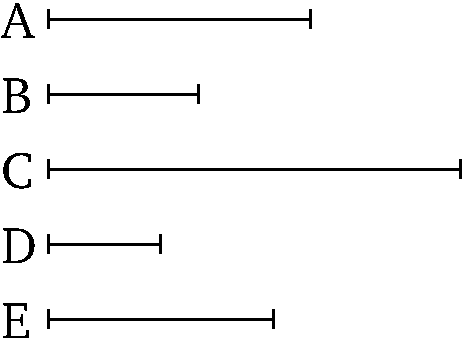
\includegraphics{Book09/fig07e.pdf}}

For let the composite number $A$ make $C$ (by) multiplying some number
$B$. I say that $C$ is  solid.

For since $A$ is a composite (number), it will be measured by some
number. Let it be measured by $D$.  And, as many times as $D$ measures
$A$, so many units let there be in $E$. Therefore, since $D$ measures $A$
according to the units in $E$, $E$ has thus made $A$ (by) multiplying
$D$ [Def.~7.15]. And since $A$ has made $C$ (by) multiplying $B$, and $A$ is
the (number created) from (multiplying) $D$, $E$, the (number created)
from (multiplying) $D$, $E$ has thus made $C$ (by) multiplying $B$. Thus,
$C$ is solid, and its sides are $D$, $E$, $B$. (Which is) the
very thing it was required to show.}
\end{Parallel}

%%%%%%
% Prop 9.8
%%%%%%
\pdfbookmark[1]{Proposition 9.8}{pdf9.8}
\begin{Parallel}{}{} 
\ParallelLText{
\begin{center}
{\large \ggn{8}.}
\end{center}\vspace*{-7pt}

\gr{Ἐὰν ἀπὸ μονάδοξ ὁποσοιοῦν ἀριθμοὶ ἑχῆξ ἀνάλογον >ῶσιν,
ὁ μὲν τρίτοξ ἀπὸ τῆξ μονάδοξ τετράγωνοξ >έσται καὶ οἱ <ένα
διαλείποντεξ, ὁ δὲ τέταρτοξ κύβοξ καὶ οἱ δύο διαλείποντεξ πάντεξ,
ὁ δὲ <έβδομοξ κύβοξ <άμα καὶ τετράγωνοξ καὶ οἱ πέντε
διαλείποντεξ.}\\~\\~\\

% Removed epsf size command
\centerline{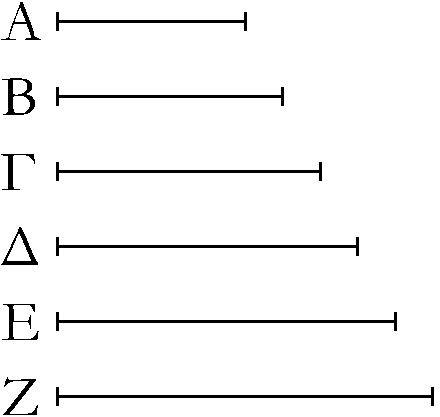
\includegraphics{Book09/fig08g.pdf}}

\gr{>'Εστωσαν ἀπὸ μονάδοξ ὁποσοιοῦν ἀριθμοὶ ἑχῆξ ἀνάλογ\-ον
οἱ Α, Β, Γ, Δ, Ε, Ζ; λέγω, <ότι ὁ μὲν τρίτοξ ἀπὸ τῆξ
μονάδοξ ὁ Β τετράγωνόξ ἐστι καὶ οἱ <ένα διαλείποντεξ πάντεξ,
ὁ δὲ τέταρτοξ ὁ Γ κύβοξ καὶ οἱ δύο διαλείποντεξ πάντεξ,
ὁ δὲ
<έβδομοξ ὁ Ζ κύβοξ <άμα καὶ τετράγωνοξ καὶ οἱ πέντε
διαλείποντεξ πάντεξ.}

\gr{Ἐπεὶ γάρ ἐστιν ὡξ ἡ μονὰξ πρὸξ τὸν Α, ο<ύτωξ ὁ Α πρὸξ τὸν Β,
ἰσάκιξ >άρα ἡ μονὰξ τὸν Α ἀριθμὸν μετρεῖ καὶ ὁ Α τὸν Β. ἡ δὲ
μονὰξ τὸν Α ἀριθμὸν μετρεῖ κατὰ τὰξ ἐν α\kern -.7pt  ὐτῶ| μονάδαξ; καὶ ὁ Α
>άρα τὸν Β μετρεῖ κατὰ τὰξ ἐν τῶ| Α μονάδαξ. ὁ Α >άρα ἑαυτὸν
πολλαπλασιάσαξ τὸν Β πεποίηκεν; τετράγωνοξ >άρα ἐστὶν ὁ Β. καὶ ἐπεὶ
οἱ Β, Γ, Δ ἑχῆξ ἀνάλογόν εἰσιν, ὁ δὲ Β τετράγωνόξ ἐστιν,
καὶ ὁ Δ >άρα τετράγωνόξ ἐστινμ\kern -.7pt  ήιὰ τὰ α\kern -.5pt  ὐτὰ δὴ καὶ ὁ Ζ
τετράγωνόξ ἐστιν. ὁμοίωξ δὴ δείχομεν, <ότι καὶ οἱ <ένα
διαλείποντεξ πάντεξ τετράγωνοί εἰσιν. λέγω δή, <ότι καὶ ὁ τέταρτοξ
ἀπὸ τῆξ μονάδοξ ὁ Γ κύβοξ ἐστὶ καὶ οἱ δύο διαλείποντεξ πάντεξ.
ἐπεὶ γάρ ἐστιν ὡξ ἡ μονὰξ πρὸξ τὸν Α, ο<ύτωξ ὁ Β πρὸξ τὸν
Γ, ἰσάκιξ >άρα ἡ μονὰξ τὸν Α ἀριθμὸν μετρεῖ καὶ ὁ Β τὸν Γ.
ἡ δὲ μονὰξ τὸν Α ἀριθμὸν μετρεῖ κατὰ τὰξ ἐν τῶ| Α μονάδαξ;
καὶ ὁ Β  >άρα τὸν Γ μετρεῖ κατὰ τὰξ ἐν τῶ| Α μονάδαξ; ὁ Α
>άρα τὸν Β πολλαπλασιάσαξ τὸν Γ πεποίηκεν. ἐπεὶ ο>ῦν ὁ Α
ἑαυτὸν μὲν πολλαπλασιάσαξ τὸν Β πεποίηκεν, τὸν δὲ Β πολλαπλασιάσαξ
τὸν Γ πεποίηκεν, κύβοξ >άρα ἐστὶν ὁ Γ. καὶ ἐπεὶ οἱ Γ, Δ, Ε, Ζ
ἑχῆξ ἀνάλογόν εἰσιν, ὁ δὲ Γ κύβοξ ἐστίν, καὶ ὁ Ζ >άρα κύβοξ
ἐστίν. ἐδείθθη δὲ καὶ τετράγωνοξ; ὁ >άρα <έβδομοξ ἀπὸ
τῆξ μονάδοξ κύβοξ τέ ἐστι καὶ τετράγωνοξ. ὁμοίωξ δὴ δείχομεν,
<ότι καὶ οἱ πέντε διαλείποντεξ πάντεξ κύβοι τέ εἰσι καὶ
τετράγωνοι; <όπερ >έδει δεῖχαι.}}

\ParallelRText{
\begin{center}
{\large Proposition 8}
\end{center}

If any multitude whatsoever of numbers is continuously proportional, (starting) from a unit, then the third from the unit will be 
square, and (all) those (numbers after that) which leave an interval of  one (number), and the fourth (will
be) cube, and all those (numbers after that) which leave an interval of two (numbers), and the seventh
(will be) both cube and square, and (all) those (numbers after that) which leave an interval of five (numbers).

% Removed epsf size command
\centerline{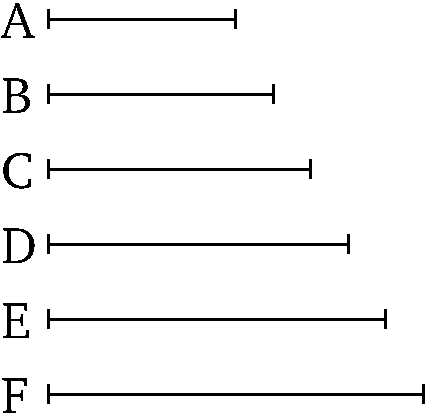
\includegraphics{Book09/fig08e.pdf}}

Let any multitude whatsoever of numbers, $A$, $B$, $C$, $D$, $E$, $F$, be continuously proportional, (starting) from a unit. I say that the third from the unit, $B$, is square, and all those (numbers after that) which leave an interval of one (number). And the fourth (from the unit), $C$,
(is)  cube, and all those (numbers after that) which leave an
interval of two (numbers). And the seventh (from the unit), $F$, (is)
both cube and square,  and all those (numbers after that) which leave an interval of five (numbers).

For since as the unit is to $A$, so $A$ (is) to $B$, the unit thus measures the number $A$
the same number of times as $A$ (measures) $B$ [Def.~7.20]. And the unit measures the number $A$
according to the units in it. Thus, $A$ also measures $B$ according to the units
in $A$. $A$ has thus made $B$ (by) multiplying itself [Def.~7.15].  Thus, $B$ is  square. And
since $B$, $C$, $D$ are continuously proportional, and $B$ is  square, $D$ is thus also  square  
[Prop.~8.22]. So, for the same (reasons), $F$ is also
 square. So, similarly, we can also show that all those (numbers after that) which leave an interval of  one (number) are square. 
So I also say that the fourth (number) from the unit, $C$,  is  cube, and
all those (numbers after that) which leave an interval of two (numbers).
For since as the unit is to $A$, so $B$ (is) to $C$, the unit thus measures the
number $A$ the same number of times that $B$ (measures) $C$. And the
unit measures the number $A$ according to the units in $A$. And thus
$B$ measures $C$ according to the units in $A$.  $A$ has thus made $C$
(by) multiplying $B$. Therefore, since $A$ has made $B$ (by) multiplying
itself, and has made $C$ (by) multiplying $B$, $C$ is thus  cube. And since $C$, $D$, $E$, $F$ are continuously proportional, and
$C$ is cube, $F$ is thus also  cube  [Prop.~8.23]. And it was also shown (to be) 
square. Thus, the seventh (number) from the unit is (both) 
cube and  square. So, similarly, we can show that  all those (numbers after that) which leave an interval of five (numbers) are (both)
cube and square. (Which is) the very thing it was required to show.}
\end{Parallel}

%%%%%%
% Prop 9.9
%%%%%%
\pdfbookmark[1]{Proposition 9.9}{pdf9.9}
\begin{Parallel}{}{} 
\ParallelLText{
\begin{center}
{\large \ggn{9}.}
\end{center}\vspace*{-7pt}

\gr{Ἐὰν ἀπὸ μονάδοξ ὁποσοιοῦν ἑχῆξ κατὰ τὸ συνεθὲξ ἀριθμοὶ
ἀνάλογον >ῶσιν, ὁ δὲ μετὰ τὴν μονάδα τετράγωνοξ >ῆ|, καὶ οἱ
λοιποὶ πάντεξ τετράγωνοι >έσονται. καὶ ἒαν ὁ μετὰ τὴν μονάδα
κύβοξ >ῆ|, καὶ οἱ λοιποὶ πάντεξ κύβοι >έσονται.}\\

% Removed epsf size command
\centerline{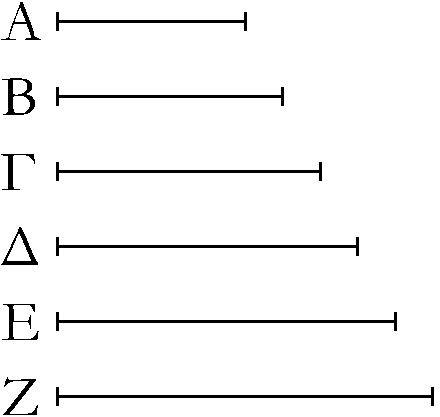
\includegraphics{Book09/fig08g.pdf}}

\gr{>'Εστωσαν ἀπὸ μονάδοξ ἑχῆξ ἀνάλογον ὁσοιδηποτοῦν ἀριθμοὶ
οἱ Α, Β, Γ, Δ, Ε, Ζ,  ὁ δὲ μετὰ τὴν μονάδα ὁ Α τετράγωνοξ
>έστω; λέγω, <ότι καὶ οἱ λοιποὶ πάντεξ τετράγωνοι >έσονται.}

\gr{<'Οτι μὲν ο>ῦν ὁ τρίτοξ ἀπὸ τῆξ μονάδοξ ὁ Β τετράγωνόξ
ἐστι καὶ οἱ <ένα διαπλείποντεξ πάντεξ, δέδεικται; λέγω [δή], <ότι
καὶ οἱ λοιποὶ πάντεξ τετράγωνοί εἰσιν. ἐπεὶ γὰρ οἱ Α, Β, Γ
ἑχῆξ ἀνάλογόν εἰσιν, καί ἐστιν ὁ Α τετράγωνοξ, καὶ ὁ Γ [>άρα]
τετράγωνοξ ἐστιν. πάλιν, ἐπεὶ [καὶ] οἱ Β, Γ, Δ ἑχῆξ ἀνάλογόν
εἰσιν, καί ἐστιν ὁ Β τετράγωνοξ, καὶ ὁ Δ [>άρα] τετράγωνόξ
ἐστιν. ὁμοίωξ δὴ δείχομεν, <ότι καὶ οἱ λοιποὶ πάντεξ
τετράγωνοί εἰσιν.}

\gr{Ἀλλὰ δὴ >έστω ὁ Α κύβοξ; λέγω, <ότι καὶ οἱ λοιποὶ πάντεξ
κύβοι εἰσίν.}

\gr{<'Οτι μὲν ο>ῦν ὁ τέταρτοξ ἀπὸ τῆξ μονάδοξ ὁ Γ κύβοξ
ἐστὶ καὶ οἱ δύο διαλείποντεξ πάντεξ, δέδεικται;
λέγω [δή], <ότι καὶ οἱ λοιποὶ πάντεξ κύβοι εἰσίν. ἐπεὶ
γάρ ἐστιν ὡξ ἡ μονὰξ πρὸξ τὸν Α, ο<ύτωξ ὁ Α πρὸξ
τὸν Β, ἰσάκιξ ἀρα ἡ μονὰξ τὸν Α μετρεῖ καὶ ὁ Α τὸν Β.
ἡ δὲ μονὰξ τὸν Α μετρεῖ κατὰ τὰξ ἐν α\kern -.7pt  ὐτῶ|
μονάδαξ; καὶ ὁ Α >άρα τὸν Β μετρεῖ κατὰ τὰξ ἐν α\kern -.7pt  ὐτῶ|
μονάδαξ; ὁ Α >άρα ἑαυτὸν πολλαπλασιάσαξ τὸν Β πεποίηκεν. καί
ἐστιν ὁ Α κύβοξ. ἒαν δὲ κύβοξ ἀριθμὸξ ἑαυτὸν πολλαπλασιάσαξ
ποιῆ| τινα, ὁ γενόμενοξ κύβοξ ἐστίν; καὶ ὁ Β >άρα κύβοξ ἐστίν.
καὶ ἐπεὶ τέσσαρεξ ἀριθμοὶ οἱ Α, Β, Γ, Δ ἑχῆξ ἀνάλογόν
εἰσιν, καί ἐστιν ὁ Α κύβοξ, καὶ ὁ Δ >άρα κύβοξ ἐστίν. διὰ
τὰ α\kern -.5pt  ὐτὰ δὴ καὶ ὁ Ε κύβοξ ἐστίν, καὶ ὁμοίωξ οἱ λοιποὶ
πάντεξ κύβοι εἰσίν; <όπερ >έδει δεῖχαι.}}

\ParallelRText{
\begin{center}
{\large Proposition 9}
\end{center}

If  any multitude whatsoever of numbers is continuously proportional, (starting) from a unit, and the (number) after the
unit is square, then all the remaining (numbers) will also 
be square. And if the (number) after the unit is  cube, then
all the remaining (numbers) will also be cube.

% Removed epsf size command
\centerline{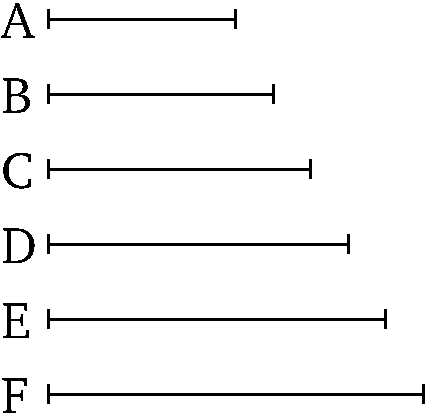
\includegraphics{Book09/fig08e.pdf}}

Let any multitude whatsoever of numbers, $A$, $B$, $C$, $D$, $E$, $F$, be continuously proportional, (starting) from a unit. And let the (number) after the
unit, $A$, be square. I say that all the remaining (numbers)
will also be square.

In fact, it has (already) been shown that the third (number) from the unit, $B$, is
square, and all those (numbers after that) which leave an interval of one (number) [Prop.~9.8]. [So] I say that all the remaining (numbers) are also square. For since $A$, $B$, $C$
are continuously proportional, and $A$ (is)  square, $C$
is [thus] also  square [Prop.~8.22]. Again, 
since $B$, $C$, $D$ are [also] continuously proportional, and $B$ is
 square, $D$ is [thus] also square [Prop.~8.22]. So, similarly,
we can show that all the remaining (numbers) are also square.

And so let $A$ be  cube. I say that all the remaining (numbers)
are also cube.

In fact, it has (already) been shown that the fourth (number) from the unit, $C$, is
cube, and all those (numbers after that) which leave an interval of two (numbers) [Prop.~9.8]. [So] I say
that all the remaining (numbers) are also cube. For since as the
unit is to $A$, so $A$ (is) to $B$, the unit thus measures $A$ the same number of times as $A$ (measures) $B$. And the unit measures $A$ according to the units in it. Thus, $A$ also measures $B$ according to the
units in ($A$).
$A$ has thus made $B$ (by) multiplying itself. 
And $A$ is  cube. And if a cube number makes some (number by)
multiplying itself then the created (number) is cube  [Prop.~9.3]. Thus, $B$ is also cube.
And since the four numbers $A$, $B$, $C$, $D$ are continuously proportional, and $A$ is  cube, $D$ is thus also  cube 
 [Prop.~8.23]. So, for the same (reasons), $E$ is also
 cube, and, similarly, all the remaining (numbers) are cube. (Which is) the very thing it was required to show.}
\end{Parallel}

%%%%%%
% Prop 9.10
%%%%%%
\pdfbookmark[1]{Proposition 9.10}{pdf9.10}
\begin{Parallel}{}{} 
\ParallelLText{
\begin{center}
{\large \ggn{10}.}
\end{center}\vspace*{-7pt}

\gr{Ἐὰν ἀπὸ μονάδοξ ὁποσοιοῦν ἀριθμοὶ [ἑχῆξ] ἀνάλογ\-ον >ῶσιν,
ὁ δὲ μετὰ τὴν μονάδα μ\kern -.7pt  ὴ >ῆ| τετράγωνοξ, οὐδ> >άλλοξ οὐδεὶξ
τετράγωνοξ >έσται θωρὶξ τοῦ τρίτου ἀπὸ τῆξ μονάδοξ
καὶ τῶν <ένα διαλειπόντων πάντων. καὶ ἒαν ὁ μετὰ τὴν μονάδα κύβοξ μ\kern -.7pt  ὴ >ῆ|, οὐδὲ >άλλοξ οὐδεὶξ κύβοξ >έσται θωρὶξ τοῦ
τετάρτου ἀπὸ τῆξ μονάδοξ καὶ τῶν δύο διαλειπόντων πάντων.}\\~\\~\\

% Removed epsf size command
\centerline{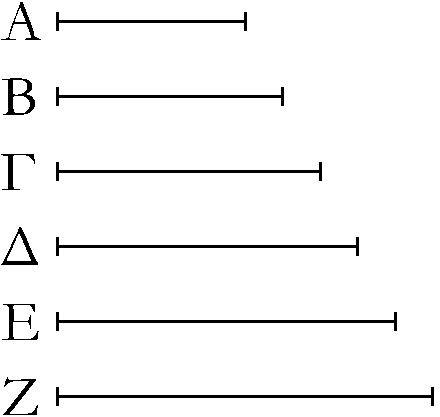
\includegraphics{Book09/fig08g.pdf}}

\gr{>'Εστωσαν ἀπὸ μονάδοξ ἑχῆξ ἀνάλογον ὁσοιδηποτοῦν ἀριθμοὶ
οἱ Α, Β, Γ, Δ, Ε, Ζ, ὁ μετὰ τὴν μονάδα ὁ Α μ\kern -.7pt  ὴ >έστω τετράγωνοξ;
λέγω, <ότι οὐδὲ >άλλοξ οὐδεὶξ τετράγωνοξ >έσται θωρὶξ τοῦ
τρίτου ἀπὸ τὴξ μονάδοξ [καὶ τῶν <ένα διαλειπόντων].}

\gr{Εἰ γὰρ δυνατόν, >έστω ὁ Γ τετράγωνοξ. >έστι δὲ καὶ ὁ Β τετράγωνοξ;
οἱ Β, Γ >άρα πρὸξ ἀλλήλουξ λόγον >έθουσιν, <ὸν τετράγωνοξ
ἀριθμὸξ πρὸξ τετράγωνον ἀριθμόν. καί ἐστιν ὡξ ὁ Β πρὸξ τὸν Γ,
ὁ Α πρὸξ τὸν Β; οἱ Α, Β >άρα πρὸξ ἀλλήλουξ λόγον >έθουσιν, <ὸν τετράγωνοξ ἀριθμὸξ πρὸξ τετράγωνον ἀριθμόν; <ώστε οἱ Α, Β
<όμοιοι ἐπίπεδοί εἰσιν. καί ἐστι τετράγωνοξ ὁ Β; τετράγωνοξ
>άρα ἐστὶ καὶ ὁ Α; <όπερ οὐθ ὑπέκειτο. οὐκ >άρα ὁ Γ τετράγωνόξ
ἐστιν. ὁμοίωξ δὴ δείχομεν, <ότι οὐδ> >άλλοξ οὐδεὶξ τετράγωνόξ
ἐστι θωρὶξ τοῦ τρίτου ἀπὸ τῆξ μονάδοξ  καὶ τῶν <ένα διαλειπόντων.}

\gr{Ἀλλὰ δὴ μ\kern -.7pt  ὴ >έστω ὁ Α κύβοξ. λέγω, <ότι οὐδ> >άλλοξ οὐδεὶξ
κύβοξ >έσται θωρὶξ τοῦ τετάρτου ἀπὸ τῆξ μονάδοξ καὶ τῶν δύο διαλειπόντων.}

\gr{Εἰ γὰρ δυνατόν, >έστω ὁ Δ κύβοξ. >έστι δὲ καὶ ὁ Γ κύβοξ;
τέταρτοξ γάρ ἐστιν ἀπὸ τῆξ μονάδοξ. καί ἐστιν ὡξ ὁ Γ πρὸξ
τὸν Δ, ὁ Β πρὸξ τὸν Γ; καὶ ὁ Β >άρα πρὸξ τὸν Γ λόγον >έθει, <ὸν
κύβοξ πρὸξ κύβον. καί ἐστιν ὁ Γ κύβοξ; καὶ ὁ Β >άρα κύβοξ
ἐστίν. καὶ ἐπεί ἐστιν ὡξ ἡ μονὰξ  πρὸξ τὸν Α, ὁ Α πρὸξ
τὸν Β, ἡ δὲ μονὰξ τὸν Α μετρεῖ κατὰ τὰξ ἐν α\kern -.7pt  ὐτῶ| μονάδαξ,
καὶ ὁ Α >άρα τὸν Β μετρεῖ κατὰ τὰξ ἐν α\kern -.7pt  ὐτῶ| μονάδαξ;
ὁ Α >άρα ἑαυτὸν πολλαπλασιάσαξ κύβον τὸν Β πεποίηκεν. ἒαν
δὲ ἀριθμὸξ ἑαυτὸν πολλαπλασιάσαξ κύβον ποιῆ|, καὶ α\kern -.5pt  ὐτὸξ κύβοξ
>έσται. κύβοξ >άρα καὶ ὁ Α; <όπερ οὐθ ὑπόκειται. οὐκ >άρα
ὁ Δ κύβοξ ἐστίν. ὁμοίωξ δὴ δείχομεν, <ότι οὐδ>
>άλλοξ οὐδεὶξ κύβοξ ἐστὶ θωρὶξ τοῦ τετάρτου ἀπὸ τῆξ
μονάδοξ καὶ τῶν δύο διαλειπόντων; <όπερ >έδει δεῖχαι.}}

\ParallelRText{
\begin{center}
{\large Proposition 10}
\end{center}

If any multitude whatsoever of numbers is [continuously] proportional, (starting) from a unit, and the (number) after the
unit is not  square, then no other (number) will be  square
either, apart from the third from the unit, and all those (numbers after that) which leave an interval of  one (number). And if the (number) after the unit is not cube, then no other (number) will be cube
 either, apart from the fourth from the unit, and all those (numbers after that) which leave an interval of  two (numbers).
 
% Removed epsf size command
\centerline{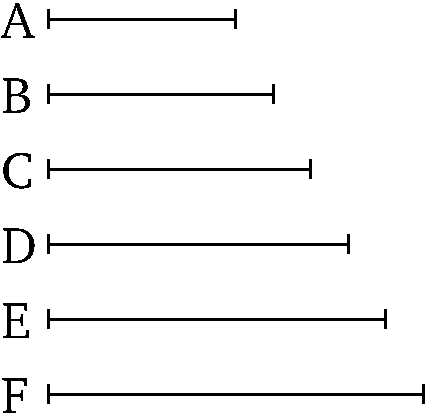
\includegraphics{Book09/fig08e.pdf}}
 
Let any multitude whatsoever of numbers, $A$, $B$, $C$, $D$, $E$, $F$, be continuously proportional, (starting) from a unit. And let the (number) after the unit, $A$, not be  square. I say that  no other (number)  will
be square either, apart from the third from the unit [and (all) those (numbers after that) which leave an interval of  one (number)].

For, if possible, let $C$ be square.  And $B$ is also square [Prop.~9.8]. Thus, $B$ and $C$ have to one another (the) ratio which (some) square number (has) to (some other) square number. And as $B$ is to $C$, (so) $A$ (is) to $B$. Thus, $A$ and $B$ have
to one another (the) ratio which (some) square number has to (some other)
square number.  Hence, $A$ and $B$ are similar plane (numbers) [Prop.~8.26]. And $B$ is square.
Thus, $A$ is also  square. The very opposite thing was assumed.
$C$ is thus not square. So, similarly, we can show that no other
(number is) square either, apart from the  third from the unit, and (all) those (numbers after that) which leave an interval of  one (number).

And so let $A$ not be  cube. I say that  no other (number)  will
be cube either, apart from the fourth from the unit, and (all) those (numbers after that) which leave an interval of  two (numbers).

For, if possible, let $D$ be  cube. And $C$ is also  cube 
[Prop.~9.8]. For it is the fourth (number) from the unit.
And as $C$ is to $D$,  (so) $B$ (is) to $C$. And $B$ thus has to $C$ the
ratio which (some) cube (number has) to (some other) cube (number). And $C$
is  cube. Thus, $B$ is also cube [Props.~7.13, 8.25].
And since as the unit is to $A$,  (so) $A$ (is) to $B$, and the unit measures
$A$ according to the units in it, $A$ thus also measures $B$ according to the units in ($A$). Thus, $A$ has made the cube  (number) $B$ (by) multiplying
itself. And if a number makes a cube (number by) multiplying itself then
it itself will be  cube  [Prop.~9.6]. Thus, $A$
(is) also  cube. The very opposite thing was assumed. Thus, $D$ is not
cube. So, similarly, we can show that no other (number) is cube
either, apart from the fourth from the unit, and (all) those (numbers after that) which leave an interval of  two (numbers). (Which is) the very thing it was required to show.}
\end{Parallel}

%%%%%%
% Prop 9.11
%%%%%%
\pdfbookmark[1]{Proposition 9.11}{pdf9.11}
\begin{Parallel}{}{} 
\ParallelLText{
\begin{center}
{\large \ggn{11}.}
\end{center}\vspace*{-7pt}

\gr{Ἐὰν ἀπὸ μονάδοξ ὁποσοιοῦν ἀριθμοὶ ἑχῆξ ἀνάλογον >ῶσιν, ὁ ἐλάττων τὸν μείζονα μετρεῖ κατά τινα τῶν ὑπαρθόντ\-ων ἐν τοῖξ
ἀνάλογον ἀριθμοῖξ.}\\

% Removed epsf size command
\centerline{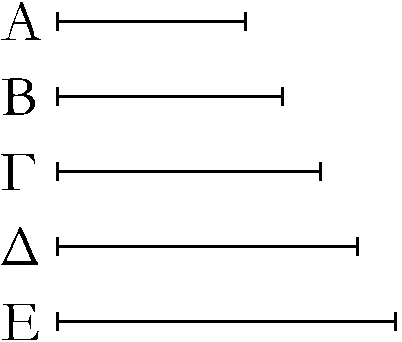
\includegraphics{Book09/fig11g.pdf}}

\gr{>'Εστωσαν ἀπὸ μονάδοξ τῆξ Α ὁποσοιοῦν ἀριθμοὶ ἑχῆξ
ἀνάλογον οἱ Β, Γ, Δ, Ε; λέγω, <ότι τῶν Β, Γ, Δ, Ε ὁ ἐλάθιστοξ
ὁ Β τὸν Ε μετρεῖ κατά τινα τῶν Γ, Δ.}

\gr{Ἐπεὶ γάρ ἐστιν ὡξ ἡ Α μονὰξ πρὸξ τὸν Β, ο<ύτωξ ὁ Δ πρὸξ
τὸν Ε, ἰσάκιξ >άρα ἡ Α μονὰξ τὸν Β ἀριθμὸν μετρεῖ καὶ ὁ Δ τὸν 
Ε; ἐναλλὰχ >άρα ἰσάκιξ ἡ Α μονὰξ τὸν Δ μετρεῖ καὶ ὁ Β τὸν Ε.
ἡ δὲ Α μονὰξ τὸν Δ μετρεῖ  κατὰ τὰξ ἐν α\kern -.7pt  ὐτῶ| μονάδαξ; καὶ ὁ Β >άρα τὸν Ε μετρεῖ κατὰ τὰξ ἐν τῶ| Δ μονάδαξ; <ώστε ὁ ἐλάσσων ὁ Β τὸν μείζονα τὸν Ε μετρεῖ κατά
τινα ἀριθμὸν τῶν ὑπαρθόντων ἐν τοῖξ ἀνάλογον ἀριθμοῖξ.}\\~\\~\\

\begin{center}
{\large \gr{Πόρισμα}.}
\end{center}\vspace*{-7pt}

\gr{Καὶ φανερόν, <ότι <ὴν >έθει τάχιν ὁ μετρῶν ἀπὸ μονάδοξ, τὴν
α\kern -.7pt  ὐτὴν >έθει καὶ ὁ καθ> <ὸν μετρεῖ ἀπὸ τοῦ μετρουμένου
ἐπὶ τὸ πρὸ α\kern -.7pt  ὐτοῦ. <όπερ >έδει δεῖχαι.}}

\ParallelRText{
\begin{center}
{\large Proposition 11}
\end{center}

If any multitude whatsoever of numbers is continuously proportional, (starting) from a unit, then a lesser (number)
measures a greater according to some existing (number)  among
the proportional numbers.

% Removed epsf size command
\centerline{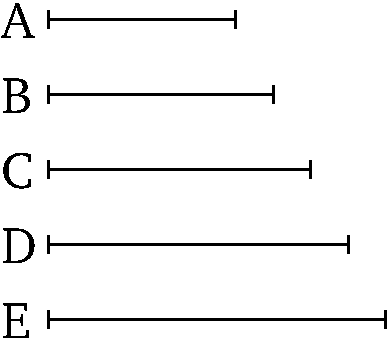
\includegraphics{Book09/fig11e.pdf}}

Let any multitude whatsoever of numbers,  $B$, $C$, $D$, $E$, be continuously proportional, (starting) from the unit $A$. I say that, for $B$, $C$, $D$, $E$, the least (number), $B$, measures $E$ according to some (one) of
$C$, $D$.

For since as the unit $A$ is to $B$, so $D$ (is) to $E$,  the unit $A$ thus measures the number $B$ the same number of times as $D$ (measures) $E$. Thus,
alternately, the unit $A$ measures $D$ the same number of times as $B$
(measures) $E$ [Prop.~7.15]. And the unit $A$ measures $D$ according to the units in it. Thus, $B$ also measures $E$ according to the units in $D$. Hence, the lesser (number) $B$
measures the greater $E$ according to some existing number among the
proportional numbers (namely, $D$). \\

\begin{center}
{\large Corollary}
\end{center}\vspace*{-7pt}

And (it is) clear that what(ever relative) place the measuring (number) has from the unit,
the  (number) according to which it measures has the same (relative) place from the measured (number), in (the direction of the number)
before it. (Which is) the very thing it was required to show.}
\end{Parallel}

%%%%%%
% Prop 9.12
%%%%%%
\pdfbookmark[1]{Proposition 9.12}{pdf9.12}
\begin{Parallel}{}{} 
\ParallelLText{
\begin{center}
{\large \ggn{12}.}
\end{center}\vspace*{-7pt}

\gr{Ἐὰν ἀπὸ μονάδοξ ὁποσοιοῦν ἀριθμοὶ ἑχῆξ ἀνάλογον >ῶσιν,
ὑφ> <όσων >ὰν ὁ >έσθατοξ πρώτων ἀριθμῶν μετρῆται, ὑπὸ
τῶν α\kern -.7pt  ὐτῶν καὶ ὁ παρὰ τὴν μονάδα μετρηθήσεται.}\\

% Removed epsf size command
\centerline{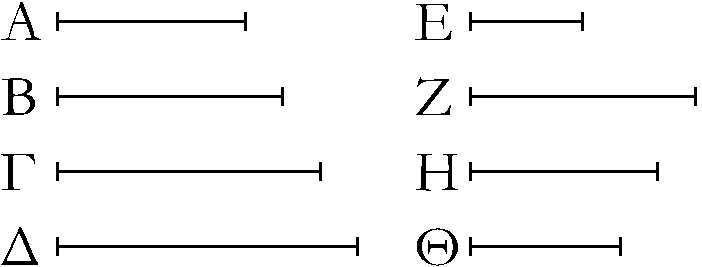
\includegraphics{Book09/fig12g.pdf}}

\gr{>'Εστωσαν ἀπὸ μονάδοξ ὁποσοιδηποτοῦν ἀριθμοὶ ἀνάλογ\-ον οἱ 
Α, Β, Γ, Δ; λέγω, <ότι ὑφ> <όσων >ὰν ὁ Δ πρώτων ἀριθμῶν μετρῆται, ὑπὸ τῶν α\kern -.7pt  ὐτῶν καὶ ὁ Α μετρηθήσεται.}

\gr{Μετρείσθω γὰρ ὁ Δ ὑπό τινοξ πρώτου ἀριθμοῦ τοῦ Ε; λέγω, <ότι
ὁ Ε τὸν Α μετρεῖ. μ\kern -.7pt  ὴ γάρ; καί ἐστιν ὁ Ε πρῶτοξ, <άπαξ δὲ πρῶτοξ
ἀριθμὸξ πρὸξ <άπαντα, <ὸν μ\kern -.7pt  ὴ μετρεῖ, πρῶτόξ ἐστιν; οἱ Ε, Α >άρα
πρῶτοι πρὸξ ἀλλήλουξ εἰσίν. καὶ ἐπεὶ ὁ Ε τὸν Δ μετρεῖ, μετρείτω
α\kern -.5pt  ὐτὸν κατὰ τὸν Ζ; ὁ Ε >άρα τὸν Ζ πολλαπλασιάσαξ τὸν Δ πεποίηκεν. πάλιν, ἐπεὶ ὁ Α τὸν Δ μετρεῖ κατὰ τὰξ ἐν τῶ| Γ μονάδαξ, ὁ 
Α  >άρα τὸν Γ πολλαπλασιάσαξ τὸν Δ πεποίηκεν. ἀλλὰ μ\kern -.3pt  ὴν καὶ ὁ Ε
τὸν Ζ πολλαπλασιάσαξ τὸν Δ πεποίηκεν; ὁ >άρα ἐκ τῶν Α, Γ >ίσοξ
ἐστὶ τῶ| ἐκ τῶν Ε, Ζ. >έστιν >άρα ὡξ ὁ Α πρὸξ τὸν Ε, ὁ Ζ
πρὸξ τὸν Γ. οἱ δὲ Α, Ε πρῶτοι, οἱ δὲ πρῶτοι καὶ ἐλάθιστοι, οἱ
δὲ ἐλάθιστοι μετροῦσι τοὺξ τὸν α\kern -.7pt  ὐτὸν λόγον >έθονταξ ἰσάκιξ
<ό τε ἡγούμενοξ τὸν ἡγούμενον καὶ ὁ ἑπόμενοξ τὸν
ἑπόμενον; μετρεῖ >άρα ὁ Ε τὸν Γ. μετρείτω α\kern -.7pt  ὐτὸν κατὰ τὸν Η;
ὁ Ε >άρα τὸν Η πολλαπλασιάσαξ τὸν Γ πεποίηκεν. ἀλλὰ μ\kern -.7pt  ὴν διὰ
τὸ πρὸ τούτου καὶ ὁ Α τὸν Β πολλαπλασιάσαξ τὸν Γ πεποίηκεν. ὁ
>άρα ἐκ τῶν Α, Β >ίσοξ ἐστὶ τῶ| ἐκ τῶν Ε, Η. >έστιν >άρα
ὡξ ὁ Α πρὸξ τὸν Ε, ὁ Η πρὸξ τὸν Β. οἱ δὲ Α, Ε πρῶτοι, οἱ
δὲ πρῶτοι καὶ ἐλάθιστοι, οἱ δὲ ἐλάθιστοι ἀριθμοὶ μετροῦσι τοὺξ
τὸν α\kern -.7pt  ὐτὸν λόγον >έθονταξ α\kern -.7pt  ὐτοῖξ ἰσάκιξ <ό τε ἡγούμενοξ
τὸν ἡγούμενον καὶ ὁ ἑπόμενοξ τὸν ἑπόμενον; μετρεῖ >άρα ὁ Ε
τὸν Β. μετρείτω α\kern -.7pt  ὐτὸν κατὰ τὸν Θ; ὁ Ε >άρα τὸν Θ πολλαπλασιάσαξ
τὸν Β πεποίηκεν. ἀλλὰ μ\kern -.7pt  ὴν καὶ ὁ Α ἑαυτὸν πολλαπλασιάσαξ τὸν Β
πεποίηκεν; ὁ >άρα ἐκ τῶν Ε, Θ >ίσοξ ἐστὶ τῶ| ἀπὸ τοῦ Α.
>έστιν >άρα ὡξ ὁ Ε πρὸξ τὸν Α, ὁ Α πρὸξ τὸν Θ. οἱ δὲ Α, Ε
πρῶτοι, οἱ δὲ πρῶτοι καὶ ἐλάθιστοι, οἱ δὲ ἐλάθιστοι μετροῦσι
τοὺξ τὸν α\kern -.7pt  ὐτὸν λόγον >έθονταξ ἰσάκιξ <ό ἡγούμενοξ τὸν ἡγούμενον καὶ ὁ ἑπόμενοξ τὸν ἑπόμενον; μετρεῖ >άρα
ὁ Ε τὸν Α ὡξ ἡγούμενοξ ἡγούμενον. ἀλλὰ μ\kern -.7pt  ὴν καὶ οὐ
μετρεῖ; <όπερ ἀδύνατον. οὐκ >άρα οἱ Ε, Α πρῶτοι πρὸξ ἀλλήλουξ
εἰσίν. σύνθετοι >άρα. οἱ δὲ σύνθετοι ὑπὸ [πρώτου] ἀριθμοῦ τινοξ
μετροῦνται. καὶ ἐπεὶ ὁ Ε πρῶτοξ ὑπόκειται, ὁ δὲ πρῶτοξ
ὑπὸ ἑτέρου ἀριθμοῦ οὐ μετρεῖται >ὴ ὑφ> ἑαυτοῦ, ὁ Ε
>άρα τοὺξ Α, Ε μετρεῖ; <ώστε ὁ Ε τὸν Α μετρεῖ. μετρεῖ δὲ καὶ
τὸν Δ; ὁ Ε >άρα τοὺξ Α, Δ μετρεῖ. ὁμοίωξ δὴ δείχομεν, <ότι
ὑφ> <όσων >ὰν ὁ Δ πρώτων ἀριθμῶν μετρῆται, ὑπὸ τῶν α\kern -.7pt  ὐτῶν
καὶ ὁ Α μετρηθήσεται; <όπερ >έδει δεῖχαι.}}

\ParallelRText{
\begin{center}
{\large Proposition 12}
\end{center}

If  any multitude whatsoever of numbers is continuously proportional, (starting) from a unit, then  however  many prime numbers  the
last (number) is measured by, the (number) next to the unit will also be measured by the same (prime numbers).

% Removed epsf size command
\centerline{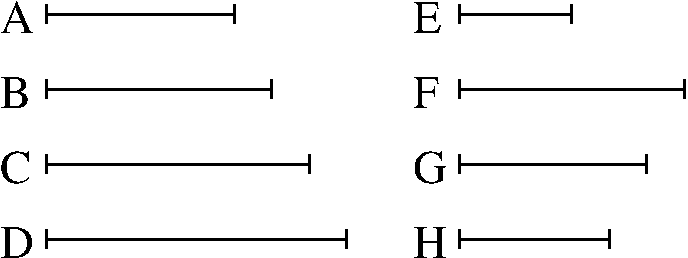
\includegraphics{Book09/fig12e.pdf}}

Let any multitude whatsoever of numbers,  $A$, $B$, $C$, $D$, be (continuously) proportional, (starting) from a unit. I say that however many prime
numbers $D$ is measured by, $A$ will also be measured by the same
(prime numbers).

For let $D$ be measured by some prime number $E$. I say that $E$ measures $A$. For (suppose it does) not. $E$ is prime, and every prime number is prime to
every number which it does not measure [Prop.~7.29]. Thus, $E$ and $A$ are prime to one another. And since $E$ measures $D$, let it measure it according to $F$. 
Thus, $E$ has made $D$ (by) multiplying $F$.  Again, since $A$ measures $D$ according to the units in $C$ [Prop.~9.11~corr.],
$A$ has thus made $D$ (by) multiplying $C$. But, in fact, $E$ has also
made $D$ (by) multiplying $F$. Thus, the (number created) from (multiplying)
$A$, $C$ is equal to  the (number created) from (multiplying) $E$, $F$.
Thus, as $A$ is to $E$, (so) $F$ (is) to $C$ [Prop.~7.19]. And $A$ and $E$ (are)  prime (to one another), and (numbers) prime (to one another are) also the least (of those
numbers having the same ratio as them) [Prop.~7.21],
and the least (numbers) measure those (numbers) having the same ratio as them an equal number of times, the leading (measuring) the leading, and the
following the following [Prop.~7.20]. Thus, $E$
measures $C$. Let it measure it according to $G$. Thus, $E$ has made $C$
(by) multiplying $G$. But, in fact, via the (proposition) before this, $A$
has also made $C$ (by) multiplying $B$ [Prop.~9.11~corr.].
 Thus, the (number created) from (multiplying) $A$, $B$ is equal to the
 (number created) from (multiplying) $E$, $G$. Thus, as $A$ is to $E$, (so) $G$ (is) to $B$ [Prop.~7.19]. And $A$ and $E$
 (are) prime (to one another), and (numbers) prime (to one another are) also the least (of those
numbers having the same ratio as them) [Prop.~7.21],
and the least (numbers) measure those (numbers) having the same ratio as them an equal number of times, the leading (measuring) the leading, and the
following the following [Prop.~7.20]. Thus, $E$
measures $B$. Let it measure it according to $H$. Thus, $E$ has made $B$ (by) multiplying $H$. But, in fact, $A$ has also made $B$
(by) multiplying itself [Prop.~9.8].  Thus, the (number created) from (multiplying) $E$, $H$ is equal to the (square) on $A$.
Thus, as $E$ is to $A$, (so) $A$ (is) to $H$ [Prop.~7.19]. And $A$ and $E$
 are prime (to one another), and (numbers) prime (to one another are) also the least (of those
numbers having the same ratio as them) [Prop.~7.21],
and the least (numbers) measure those (numbers) having the same ratio  as them an equal number of times, the leading (measuring) the leading, and the
following the following
[Prop.~7.20]. Thus, $E$
measures $A$, as the leading (measuring the) leading. But, in fact, 
($E$) also does not measure ($A$). The very thing (is) impossible. Thus,
$E$ and $A$ are not prime to one another. Thus, (they are) composite (to one another). And (numbers) composite (to one another) are (both) measured
by some [prime] number [Def.~7.14]. And since $E$
is assumed (to be) prime, and a prime (number) is not measured by  another number (other) than itself
[Def.~7.11], $E$ thus measures (both) $A$ and $E$. Hence, $E$ measures $A$. And it also measures $D$. Thus, $E$ measures (both) $A$ and $D$. So, similarly, we can show that however many prime
numbers $D$ is measured by, $A$ will also be measured by the same
(prime numbers). (Which is) the very thing it was required to show.}
\end{Parallel}

%%%%%%
% Prop 9.13
%%%%%%
\pdfbookmark[1]{Proposition 9.13}{pdf9.13}
\begin{Parallel}{}{} 
\ParallelLText{
\begin{center}
{\large \ggn{13}.}
\end{center}\vspace*{-7pt}

\gr{Ἐὰν ἀπὸ μονάδοξ ὁποσοιοῦν ἀριθμοὶ ἑχῆξ ἀνάλογον >ῶσιν,
ὁ δὲ μετὰ τὴν μονάδα πρῶτοξ >ῆ|, ὁ μέγιστοξ ὑπ> οὐδενὸξ 
[>άλλου] μετρηθήσεται παρὲχ τῶν ὑπαρθόντων  ἐν τοῖξ ἀνάλογον
ἀριθμοῖξ.}

\gr{>'Εστωσαν ἀπὸ μονάδοξ ὁποσοιοῦν ἀριθμοὶ ἑχῆξ ἀνάλογον οἱ 
Α, Β, Γ, Δ, ὁ δὲ μετὰ τὴν μονάδα ὁ Α πρῶτοξ >έστω; λέγω, <ότι
ὁ μέγιστοξ α\kern -.7pt  ὐτῶν ὁ Δ ὑπ> οὐδενὸξ >άλλου μετρηθήσεται
παρὲχ τῶν Α, Β, Γ.}\\~\\

% Removed epsf size command
\centerline{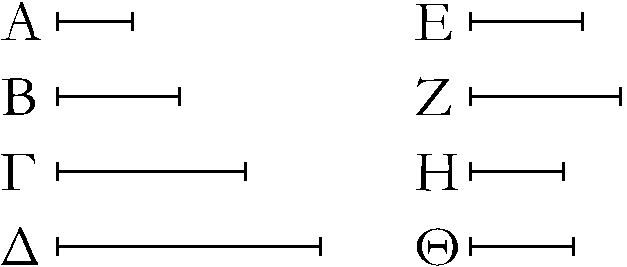
\includegraphics{Book09/fig13g.pdf}}

\gr{Εἰ γὰρ δυνατόν, μετρείσθω ὑπὸ τοῦ Ε, καὶ ὁ Ε μ\kern -.7pt  ηδενὶ τῶν Α, Β, Γ
>έστω ὁ α\kern -.7pt  ὐτόξ. φανερὸν δή, <ότι ὁ Ε πρῶτοξ ο>ύκ ἐστιν. εἰ 
γὰρ ὁ Ε πρῶτόξ ἐστι καὶ μετρεῖ τὸν Δ, καὶ τὸν Α μετρήσει
πρῶτον >όντα μ\kern -.5pt  ὴ >ὼν α\kern -.3pt  ὐτῶ| ὁ α\kern -.7pt  ὐτόξ; <όπερ ἐστὶν ἀδύνατον.
οὐκ >άρα ὁ Ε πρῶτόξ ἐστιν. σύνθετοξ >άρα. πᾶξ δὲ σύνθετοξ ἀριθμὸξ
ὑπὸ πρώτου τινὸξ ἀριθμοῦ μετρεῖται; ὁ Ε >άρα ὑπὸ πρώτου τινὸξ
ἀριθμοῦ μετρεῖται.
λέγω δή, <ότι ὑπ> οὐδενὸξ
>άλλου πρώτου μετρηθήσεται πλὴν τοῦ Α. εἰ γὰρ ὑφ> ἑτέρου μετρεῖται
ὁ Ε, ὁ δὲ Ε τὸν Δ μετρεῖ, κἀκεῖνοξ >άρα τὸν Δ μετρήσει; <ώστε καὶ
τὸν Α  μετρήσει πρῶτον >όντα μ\kern -.7pt  ὴ >ὼν α\kern -.7pt  ὐτῶ| ὁ α\kern -.7pt  ὐτόξ; <όπερ
ἐστὶν ἀδύνατον. ὁ Α >άρα τὸν  Ε μετρεῖ. καὶ ἐπεὶ ὁ Ε τὸν Δ
μετρεῖ, μετρείτω α\kern -.7pt  ὐτὸν κατὰ τὸν Ζ. λέγω, <ότι ὁ Ζ οὐδενὶ τῶν
Α, Β, Γ ἐστιν ὁ α\kern -.7pt  ὐτόξ. εἰ γὰρ ὁ Ζ ἑνὶ τῶν Α, Β, Γ ἐστιν ὁ
α\kern -.7pt  ὐτὸξ καὶ μετρεῖ τὸν Δ κατὰ τὸν Ε, καὶ ε<ῖξ >άρα τῶν Α, Β, Γ
τὸν Δ μετρεῖ κατά τὸν Ε. ἀλλὰ ε~ἱξ τῶν Α, Β, Γ τὸν Δ μετρεῖ κατά
τινα τῶν Α, Β, Γ; καὶ ὁ Ε >άρα ἑνὶ τῶν Α, Β, Γ
ἐστιν ὁ α\kern -.7pt  ὐτόξ; <όπερ οὐθ ὑπόκειται. οὐκ >άρα ὁ Ζ ἑνὶ τῶν
Α, Β, Γ ἐστιν ὁ α\kern -.7pt  ὐτόξ. ὁμοίωξ δὴ δείχομεν, <ότι μετρεῖται ὁ Ζ
ὑπὸ τοῦ Α, δεικνύντεξ πάλιν, <ότι ὁ Ζ ο>ύκ ἐστι πρῶτοξ. εἰ γὰρ,
καὶ μετρεῖ τὸν Δ, καὶ τὸν Α μετρήσει πρῶτον >όντα μ\kern -.7pt  ὴ >ὼν α\kern -.7pt  ὐτῶ|
ὁ α\kern -.7pt  ὐτόξ; <όπερ ἐστὶν ἀδύνατον; οὐκ >άρα πρῶτόξ ἐστιν ὁ Ζ;
σύνθετοξ >άρα. <άπαξ δὲ σύνθετοξ ἀριθμὸξ ὑπὸ πρώτου τινὸξ ἀριθμοῦ
μετρεῖται; ὁ Ζ >άρα ὑπὸ πρώτου τινὸξ ἀριθμοῦ μετρεῖται. λέγω δή,
<ότι ὑφ> ἑτέρου πρώτου οὐ μετρηθήσεται πλὴν τοῦ Α. εἰ γὰρ <έτερόξ
τιξ πρῶτοξ τὸν Ζ μετρεῖ, ὁ δὲ Ζ τὸν Δ μετρεῖ, κἀκεῖνοξ >άρα τὸν Δ
μετρήσει; <ώστε καὶ τὸν Α μετρήσει πρῶτον >όντα μ\kern -.7pt  ὴ >ὼν α\kern -.7pt  ὐτῶ|
ὁ α\kern -.7pt  ὐτόξ; <όπερ ἐστὶν ἀδύνατον. ὁ Α >άρα τὸν Ζ μετρεῖ. καὶ ἐπεὶ
ὁ Ε τὸν Δ μετρεῖ κατὰ τὸν Ζ, ὁ Ε >άρα τὸν Ζ πολλαπλασιάσαξ
τὸν Δ πεποίηκεν. ἀλλὰ μ\kern -.7pt  ὴν καὶ ὁ Α τὸν Γ πολλαπλασιάσαξ
τὸν Δ πεποίηκεν; ὁ >άρα ἐκ τῶν Α, Γ >ίσοξ ἐστὶ τῶ| ἐκ τῶν 
Ε, Ζ. ἀνάλογον >άρα ἐστὶν ὡξ ὁ Α πρὸξ τὸν Ε, ο<ύτωξ ὁ Ζ
πρὸξ τὸν Γ. ὁ δὲ Α τὸν Ε μετρεῖ; καὶ ὁ Ζ >άρα τὸν Γ μετρεῖ. μετρείτω α\kern -.7pt  ὐτὸν κατὰ τὸν Η. ὁμοίωξ δὴ δείχομεν, <ότι 
ὁ Η οὐδενὶ τῶν Α, Β ἐστιν ὁ α\kern -.7pt  ὐτόξ, καὶ <ότι μετρεῖται ὑπὸ
τοῦ Α. καὶ ἐπεὶ ὁ Ζ τὸν Γ μετρεῖ κατὰ τὸν Η,  ὁ Ζ >άρα τὸν Η
πολλαπλασιάσαξ τὸν Γ πεποίηκεν. ἀλλὰ μ\kern -.7pt  ὴν καὶ ὁ Α τὸν Β πολλαπλασιάσαξ
τὸν Γ πεποίηκεν; ὁ >άρα ἐκ τῶν Α, Β >ίσοξ ἐστὶ τῶ| ἐκ τῶν Ζ, Η.
ἀνάλογον >άρα ὡξ ὁ Α πρὸξ τὸν Ζ, ὁ Η πρὸξ τὸν  Β.  μετρεῖ δὲ ὁ
Α τὸν Ζ; μετρεῖ >άρα καὶ ὁ Η τὸν Β. μετρείτω
α\kern -.7pt  ὐτὸν κατὰ τὸν Θ. ὁμοίωξ δὴ
δείχομεν, <ότι ὁ Θ τῶ| Α οὐκ >έστιν
ὁ α\kern -.7pt  ὐτόξ. καὶ ἐπεὶ ὁ Η τὸν Β μετρεῖ κατὰ τὸν Θ,  ὁ Η >άρα τὸν
Θ πολλαπλασιάσαξ τὸν Β πεποίηκεν. ἀλλὰ μ\kern -.7pt  ὴν καὶ ὁ Α ἑαυτὸν πολλαπλασιάσαξ τὸν Β πεποίηκεν; ὁ >άρα ὑπὸ Θ, Η >ίσοξ ἐστὶ τῶ|
ἀπὸ τοῦ Α τετραγώνῳ;  >έστιν >άρα ὡξ ὁ Θ πρὸξ τὸν Α, ὁ Α
πρὸξ τὸν Η. μετρεῖ δὲ ὁ Α τὸν Η; μετρεῖ >άρα καὶ ὁ Θ τὸν Α
πρῶτον >όντα μ\kern -.7pt  ὴ >ὼν α\kern -.7pt  ὐτῶ| ὁ α\kern -.7pt  ὐτόξ; <όπερ >άτοπον.
οὐκ >άρα ὁ μέγιστοξ ὁ Δ ὑπὸ ἑτέρου ἀριθμοῦ μετρηθήσεται
παρὲχ τῶν Α, Β, Γ; <όπερ >έδει δεῖχαι.}}

\ParallelRText{
\begin{center}
{\large Proposition 13}
\end{center}

If  any multitude whatsoever of numbers is continuously proportional, (starting) from a unit, and the (number) after the
unit is prime, then the greatest (number) will be measured by no [other] (numbers) except (numbers) existing  among the proportional numbers.

Let any multitude whatsoever of numbers,  $A$, $B$, $C$, $D$, be continuously proportional, (starting) from a unit. And let the (number)
after the unit, $A$, be prime. I say that the greatest of them, $D$, will be
measured by no other (numbers) except $A$, $B$, $C$. 

% Removed epsf size command
\centerline{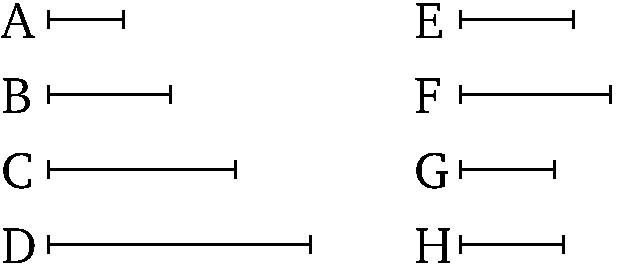
\includegraphics{Book09/fig13e.pdf}}

For, if possible, let it be measured by $E$, and let $E$ not be
the same as one of $A$, $B$, $C$. So it is clear that $E$ is not prime. 
For if $E$ is prime, and measures $D$, then it will also measure $A$, (despite $A$) being prime (and) not being  the same as it [Prop.~9.12]. The very thing is impossible. Thus, $E$
is not prime. Thus, (it is) composite. And every composite
number is measured by some prime number [Prop.~7.31]. Thus, $E$ is measured by some prime number. So I say that it will be measured by no other prime number than $A$.
For if $E$ is measured by another (prime number), and $E$ measures $D$, then this (prime number) will thus also measure $D$. Hence, it will also
measure $A$,  (despite $A$) being prime (and) not being  the same as it [Prop.~9.12]. The very thing is impossible. Thus,
$A$ measures $E$. And since $E$ measures $D$, let it measure it according to $F$. I say that $F$ is not the same as one of $A$, $B$, $C$. For if $F$ is
the same as one of $A$, $B$, $C$, and measures $D$ according to $E$,
then one of $A$, $B$, $C$ thus also measures $D$ according to $E$.
But one of $A$, $B$, $C$ (only) measures $D$ according to some (one) of
$A$, $B$, $C$
[Prop.~9.11]. And thus $E$ is the same as one of
$A$, $B$, $C$. The very opposite thing was assumed. Thus, $F$ is not the
same as one of $A$, $B$, $C$. Similarly, we can show that $F$ is measured by $A$,  (by) again showing that $F$ is not prime. For if ($F$ is prime), and measures $D$,  then it will also measure $A$, (despite $A$) being prime (and) not being  the same as it [Prop.~9.12]. The very thing
is impossible. Thus, $F$ is not prime. Thus, (it is) composite.  And every composite
number is measured by some prime number [Prop.~7.31]. Thus, $F$ is measured by some prime
number. So I say that it will be measured by no other prime number than $A$.
For if  some other prime (number) measures $F$, and $F$ measures $D$, then this (prime number) will thus also measure $D$.  Hence, it will also
measure $A$,  (despite $A$) being prime (and) not being  the same as it [Prop.~9.12]. The very thing is impossible.
Thus, $A$ measures $F$. And since $E$ measures $D$ according to 
$F$, $E$ has thus made $D$ (by) multiplying $F$.  But, in fact, $A$ has
also made $D$ (by) multiplying $C$ [Prop.~9.11~corr.]. Thus, the (number created) from (multiplying)
$A$, $C$ is equal to  the (number created) from (multiplying) $E$, $F$. Thus, proportionally, as $A$ is to $E$, so $F$ (is) to $C$ [Prop.~7.19]. And $A$ measures $E$. Thus, $F$ also
measures $C$. Let it
 measure it according to $G$. So, similarly, we can show
that $G$ is not the same as one of $A$, $B$, and that it is measured by $A$. 
And since $F$ measures $C$ according to $G$, $F$ has thus made
$C$ (by) multiplying $G$.  But, in fact, $A$ has
also made $C$ (by) multiplying $B$ [Prop.~9.11~corr.]. Thus, the (number created) from (multiplying)
$A$, $B$ is equal to  the (number created) from (multiplying) $F$, $G$.
Thus, proportionally, as $A$ (is) to $F$, so $G$ (is) to $B$ [Prop.~7.19]. And $A$ measures $F$. 
Thus, $G$ also measures $B$.
Let it measure
it according to $H$. So, similarly, we can show that $H$ is not the same as $A$. And since $G$ measures $B$ according to $H$, $G$ has thus made $B$
(by) multiplying $H$.  But, in fact, $A$ has
 also made $B$ (by) multiplying itself [Prop.~9.8]. Thus, the (number created) from (multiplying)
$H$, $G$ is equal to  the square on $A$. Thus, as $H$ is to $A$, (so) $A$ (is) to $G$ [Prop.~7.19]. And $A$ measures $G$.
Thus, $H$ also measures $A$, (despite $A$) being prime (and) not being  the same as it. The very thing (is) absurd. Thus, the greatest (number) $D$ cannot be
measured by  another (number) except (one of) $A$, $B$, $C$. (Which is) the
very thing it was required to show.}
\end{Parallel}

%%%%%%
% Prop 9.14
%%%%%%
\pdfbookmark[1]{Proposition 9.14}{pdf9.14}
\begin{Parallel}{}{} 
\ParallelLText{
\begin{center}
{\large \ggn{14}.}
\end{center}\vspace*{-7pt}

\gr{Ἐὰν ἐλάθιστοξ ἀριθμὸξ ὑπὸ πρώτων ἀριθμῶν μετρῆται, ὑπ>
οὑδενὸξ >άλλου πρώτου ἀριθμοῦ μετρηθήσεται παρὲχ τῶν ἐχ
ἀρθῆξ μετρούντων.}

\gr{Ἐλάθιστοξ γὰρ ἀριθμὸξ ὁ Α ὑπὸ πρώτων ἀριθμῶν τῶν Β, Γ, Δ
μετρείσθω; λέγω, <ότι ὁ Α ὑπ> οὐδενὸξ >άλλου πρώτου
ἀριθμοῦ μετρηθήσεται παρὲχ τῶν Β, Γ, Δ.}

% Removed epsf size command
\centerline{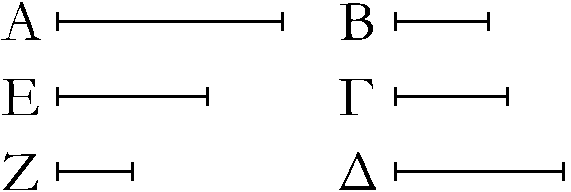
\includegraphics{Book09/fig14g.pdf}}

\gr{Εἰ γὰρ δυνατόν, μετρείσθω ὑπὸ πρώτου τοῦ Ε, καὶ ὁ Ε μ\kern -.7pt  ηδενὶ
τῶν Β, Γ, Δ >έστω ὁ α\kern -.7pt  ὐτόξ. καὶ ἐπεὶ ὁ Ε τὸν Α μετρεῖ, μετρείτω
α\kern -.5pt  ὐτὸν κατὰ τὸν Ζ; ὁ Ε >άρα τὸν Ζ πολλαπλασιάσαξ τὸν Α πεποίηκεν.
καὶ μετρεῖται ὁ Α ὑπὸ πρώτων ἀριθμῶν τῶν Β, Γ, Δ. ἒαν
δὲ δύο ἀριθμοὶ πολλαπλασιάσαντεξ ἀλλήλουξ ποιῶσί τινα, τὸν δὲ
γενόμενον ἐχ α\kern -.3pt  ὐτῶν μετρῆ| τιξ πρῶτοξ ἀριθμόξ, καὶ
<ένα τῶν ἐχ ἀρθῆξ μετρήσει; οἱ Β, Γ, Δ >άρα <ένα τῶν Ε, Ζ
μετρήσουσιν. τὸν  μὲν ο>ῦν Ε οὐ μετρήσουσιν; ὁ γὰρ Ε πρῶτόξ
ἐστι καὶ οὐδενὶ τῶν Β, Γ, Δ ὁ α\kern -.7pt  ὐτόξ. τὸν Ζ >άρα μετροῦσιν
ἐλάσσονα >όντα τοῦ Α; <όπερ ἀδύνατον. ὁ γὰρ Α ὑπόκειται
ἐλάθιστοξ ὑπὸ τῶν Β, Γ, Δ μετρούμενοξ. οὐκ >άρα τὸν
Α μετρήσει πρῶτοξ ἀριθμὸξ παρὲχ τῶν Β, Γ, Δ; <όπερ
>έδει δεῖχαι.}}

\ParallelRText{
\begin{center}
{\large Proposition 14}
\end{center}

If  a least number is measured by (some) prime numbers then it will not be measured by
any other prime number except (one of) the original measuring (numbers).

For let $A$ be the least number measured by the prime numbers $B$, $C$, $D$. I say that $A$ will not be measured by any other prime number except
(one of) $B$, $C$, $D$.

% Removed epsf size command
\centerline{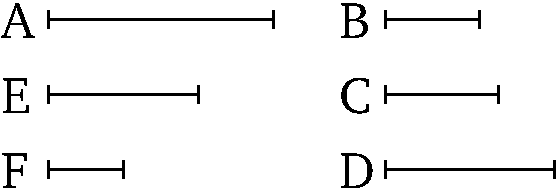
\includegraphics{Book09/fig14e.pdf}}

For, if possible, let it be measured by the prime (number) $E$. And
let $E$ not be the same as one of $B$, $C$, $D$. And since $E$ measures
$A$, let it measure it according to $F$.  Thus, $E$ has made $A$ (by)
multiplying $F$. And $A$ is measured by the prime numbers $B$, $C$, $D$.
And if two numbers make some (number by) multiplying one another,
and some prime number  measures the number created from them, then (the prime number)
will also measure one of the original (numbers) [Prop.~7.30]. Thus, $B$, $C$, $D$ will measure one of
$E$, $F$. In fact, they do not measure $E$. For $E$ is prime, and not the
same as one of $B$, $C$, $D$. Thus, they (all) measure $F$, which is less than $A$. The very thing (is) impossible. For $A$ was assumed
(to be) the least (number) measured by $B$, $C$, $D$. Thus, no prime number can measure $A$ except (one of) $B$, $C$, $D$. (Which is) the very thing it was required to show.}
\end{Parallel}

%%%%%%
% Prop 9.15
%%%%%%
\pdfbookmark[1]{Proposition 9.15}{pdf9.15}
\begin{Parallel}{}{} 
\ParallelLText{
\begin{center}
{\large \ggn{15}.}
\end{center}\vspace*{-7pt}

\gr{Ἐὰν τρεῖξ ἀριθμοὶ ἑχῆξ ἀνάλογον >ῶσιν ἐλάθιστοι τῶν τὸν
α\kern -.7pt  ὐτὸν λόγον ἐθόντων α\kern -.7pt  ὐτοῖξ, δύο ὁποιοιοῦν συντεθέντεξ πρὸξ
τὸν λοιπὸν πρῶτοί εἰσιν.}\\

% Removed epsf size command
\centerline{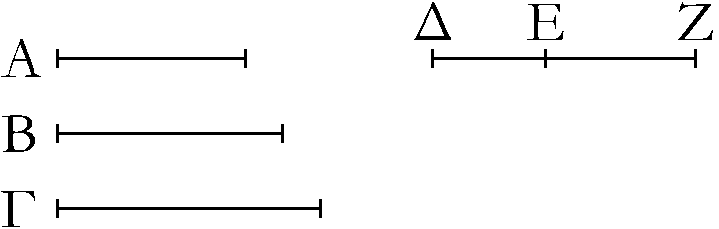
\includegraphics{Book09/fig15g.pdf}}

\gr{>'Εστωσαν τρεῖξ ἀριθμοὶ ἑχῆξ ἀνάλογον ἐλάθιστοι τῶν τὸν α\kern -.7pt  ὐτὸν
λόγον ἐθόντων α\kern -.7pt  ὐτοῖξ οἱ Α, Β, Γ;
λέγω, <ότι τῶν Α, Β, Γ δύο ὁποιοιοῦν συντεθέντεξ
πρὸξ τὸν λοιπὸν πρῶτοι εἰσιν, οἱ μὲν Α, Β πρὸξ τὸν Γ, οἱ δὲ
Β, Γ πρὸξ τὸν Α καὶ >έτι οἱ Α, Γ πρὸξ τὸν Β.}

\gr{Εἰλήφθωσαν γὰρ ἐλάθιστοι ἀριθμοὶ τῶν τὸν α\kern -.7pt  ὐτὸν λόγον
ἐθόντων τοῖξ Α, Β, Γ δύο οἱ ΔΕ, ΕΖ. φανερὸν δή, <ότι ὁ μὲν
ΔΕ ἑαυτὸν πολλαπλασιάσαξ τὸν Α πεποίηκεν, τὸν δὲ ΕΖ πολλαπλασιάσαξ
τὸν Β πεποίηκεν, καὶ >έτι ὁ ΕΖ ἑαυτὸν πολλαπλασιάσαξ τὸν Γ πεποίηκεν.
καὶ ἐπεὶ οἱ ΔΕ, ΕΖ ἐλάθιστοί εἰσιν, πρῶτοι πρὸξ ἀλλήλουξ εἰσίν.
ἒαν δὲ δύο ἀριθμοὶ πρῶτοι πρὸξ ἀλλήλουξ >ῶσιν, καὶ
συναμφότεροξ πρὸξ ἑκάτερον πρῶτόξ ἐστιν; καὶ ὁ ΔΖ >άρα
πρὸξ ἑκάτερον τῶν ΔΕ, ΕΖ πρῶτόξ ἐστιν. ἀλλὰ μ\kern -.7pt  ὴν καὶ ὁ ΔΕ
πρὸξ τὸν ΕΖ πρῶτόξ ἐστιν; οἱ ΔΖ, ΔΕ >άρα πρὸξ τὸν ΕΖ πρῶτοί
εἰσιν. ἒαν δὲ δύο ἀριθμοὶ πρόξ τινα ἀριθμὸν πρῶτοι >ῶσιν, καὶ
ὁ ἐχ α\kern -.5pt  ὐτῶν γενόμενοξ πρὸξ τὸν λοιπὸν πρῶτόξ ἐστιν; <ώστε
ὁ ἐκ τῶν ΖΔ, ΔΕ πρὸξ τὸν ΕΖ πρῶτόξ ἐστιν; <ώστε καὶ ὁ ἐκ
τῶν ΖΔ, ΔΕ πρὸξ τὸν ἀπὸ τοῦ ΕΖ πρῶτόξ ἐστιν. [ἒαν
γὰρ δύο ἀριθμοὶ πρῶτοι πρὸξ ἀλλήλουξ >ῶσιν, ὁ ἐκ τοῦ ἑνὸξ
α\kern -.3pt  ὐτῶν γενόμενοξ πρὸξ τὸν λοιπὸν πρῶτόξ ἐστιν]. ἀλλ> ὁ ἐκ
τῶν ΖΔ, ΔΕ ὁ ἀπὸ τοῦ ΔΕ ἐστι μετὰ τοῦ ἐκ τῶν ΔΕ, ΕΖ; ὁ
>άρα ἀπὸ τοῦ ΔΕ μετὰ τοῦ ἐκ τῶν ΔΕ, ΕΖ πρὸξ τὸν ἀπὸ τοῦ
 ΕΖ πρῶτόξ
ἐστιν. καί ἐστιν ὁ μὲν ἀπὸ τοῦ ΔΕ ὁ Α, ὁ δὲ ἐκ τῶν ΔΕ, ΕΖ
ὁ Β, ὁ δὲ ἀπὸ τοῦ ΕΖ ὁ Γ; οἱ Α, Β >άρα συντεθέντεξ πρὸξ τὸν Γ
πρῶτοί εἰσιν. ὁμοίωξ δὴ δείχομεν, <ότι καὶ οἱ Β, Γ
πρὸξ τὸν Α πρῶτοί εἰσιν. λέγω δή, <ότι καὶ οἱ Α, Γ πρὸξ τὸν Β πρῶτοί εἰσιν.
ἐπεὶ γὰρ ὁ ΔΖ πρὸξ ἑκάτερον
τῶν ΔΕ, ΕΖ πρῶτόξ ἐστιν, καὶ ὁ ἀπὸ τοῦ ΔΖ πρὸξ τὸν ἐκ τῶν
ΔΕ, ΕΖ πρῶτόξ ἐστιν. ἀλλὰ τῶ| ἀπὸ τοῦ ΔΖ >ίσοι
εἰσὶν οἱ ἀπὸ τῶν ΔΕ, ΕΖ μετὰ τοῦ δὶξ ἐκ τῶν ΔΕ, ΕΖ; καὶ
οἱ ἀπὸ τῶν ΔΕ, ΕΖ >άρα μετὰ τοῦ δὶξ ὑπὸ τῶν ΔΕ, ΕΖ πρὸξ
τὸν ὑπὸ τῶν ΔΕ, ΕΖ πρῶτοί [εἰσι]. διελόντι οἱ ἀπὸ τῶν ΔΕ, ΕΖ
μετὰ τοῦ <άπαχ ὑπὸ ΔΕ, ΕΖ πρὸξ τὸν ὑπὸ ΔΕ, ΕΖ πρῶτοί
εἰσιν. >έτι διελόντι οἱ ἀπὸ τῶν ΔΕ, ΕΖ >άρα πρὸξ τὸν 
ὑπὸ ΔΕ, ΕΖ πρῶτοί εἰσιν. καί ἐστιν ὁ μὲν ἀπὸ τοῦ ΔΕ ὁ
Α, ὁ δὲ ὑπὸ τῶν ΔΕ, ΕΖ ὁ Β, ὁ δὲ ἀπὸ τοῦ ΕΖ ὁ Γ. οἱ
Α, Γ >άρα συντεθέντεξ πρὸξ τὸν Β πρῶτοί εἰσιν; <όπερ >έδει
δεῖχαι.}}

\ParallelRText{
\begin{center}
{\large Proposition 15}
\end{center}

If three continuously proportional
numbers are the least of those (numbers) having the same ratio as them then
two (of them) added together in any way are prime to the remaining (one).

% Removed epsf size command
\centerline{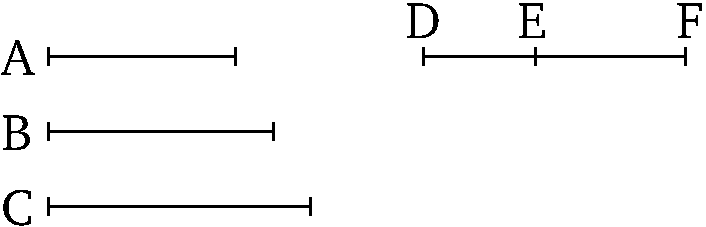
\includegraphics{Book09/fig15e.pdf}}

Let $A$, $B$, $C$ be three continuously proportional numbers (which are)
the least of those (numbers) having the same ratio as them. I say that two
of $A$, $B$, $C$ added together in any way are prime to the remaining
(one), (that is) $A$ and $B$ (prime) to $C$, $B$ and $C$ to
$A$, and, further, $A$ and $C$ to $B$.

Let the two least numbers, $DE$ and $EF$, having the same ratio as
$A$, $B$, $C$, be taken [Prop.~8.2]. So
it is clear that $DE$ has made $A$ (by) multiplying itself, and
has made $B$ (by) multiplying $EF$, and, further, $EF$ has made $C$ (by)
multiplying itself [Prop.~8.2]. And since $DE$, $EF$ are the least (of those numbers having the same ratio as them), 
they are prime to one another [Prop.~7.22]. 
And if two numbers are prime to one another then the sum (of them)
is also prime to each [Prop.~7.28]. Thus, $DF$
is also prime to each of $DE$, $EF$. But, in fact, $DE$ is  also prime to $EF$.
Thus, $DF$, $DE$ are (both) prime to $EF$. And if two numbers are (both)
prime to some number then the (number) created from (multiplying) them
is also prime to the remaining (number) [Prop.~7.24].
Hence, the (number created) from (multiplying) $FD$, $DE$ is prime
to $EF$. Hence, the (number created) from (multiplying) $FD$, $DE$ is also prime
to the (square) on $EF$ [Prop.~7.25]. 
[For if two numbers are prime to one another then the (number) created from
(squaring) one of them is prime to the remaining (number).]
But the (number created) from (multiplying) $FD$, $DE$ is the
(square) on $DE$ plus the (number created) from (multiplying) $DE$, $EF$
[Prop.~2.3]. Thus, the (square) on $DE$ plus
the (number created) from (multiplying) $DE$, $EF$ is prime to the
(square) on $EF$. 
And the (square)
on $DE$ is $A$, and the (number created) from (multiplying) $DE$, $EF$
(is) $B$, and the (square) on $EF$ (is) $C$. Thus,  $A$, $B$ summed is prime to $C$. So,  similarly, we can show that $B$, $C$ (summed) is also
prime to $A$. So I say that $A$, $C$ (summed) is also prime to $B$.
For since $DF$ is prime to each of $DE$, $EF$ then the (square) on
$DF$ is also prime to the (number created) from (multiplying) $DE$, $EF$
[Prop.~7.25]. But, the (sum of the squares) on $DE$, $EF$
plus twice the (number created) from (multiplying) $DE$, $EF$ is equal to
the (square) on $DF$ [Prop.~2.4]. And thus
the (sum of the squares) on $DE$, $EF$ plus twice  the (rectangle contained) by $DE$, $EF$ [is] prime to the (rectangle contained) by $DE$, $EF$.
By separation, the (sum of the squares) on $DE$, $EF$ plus  once the (rectangle contained) by $DE$, $EF$  is prime to the (rectangle contained)  by $DE$, $EF$.$^\dag$ Again, by separation,  the (sum of the squares) on $DE$, $EF$ is prime to the (rectangle contained)  by $DE$, $EF$. And the (square) on $DE$   is $A$,  and the (rectangle contained) by $DE$, $EF$ (is) $B$, and the (square) on $EF$ (is) $C$. Thus, $A$, $C$
summed is prime to $B$. (Which is) the very thing it was required to show.}
\end{Parallel}
{\footnotesize\noindent$^\dag$ Since if $\alpha\,\beta$ measures
$\alpha^2+\beta^2+2\,\alpha\,\beta$ then it also measures $\alpha^2+\beta^2+\alpha\,\beta$, and vice versa.}

%%%%%%
% Prop 9.16
%%%%%%
\pdfbookmark[1]{Proposition 9.16}{pdf9.16}
\begin{Parallel}{}{} 
\ParallelLText{
\begin{center}
{\large \ggn{16}.}
\end{center}\vspace*{-7pt}

\gr{Ἐὰν δύο ἀριθμοὶ πρῶτοι πρὸξ ἀλλήλουξ >ῶσιν, οὐκ >έσται ὡξ
ὁ πρῶτοξ πρὸξ τὸν δεύτερον, ο<ύτωξ ὁ δεύτεροξ πρὸξ >άλλον τινά.}

% Removed epsf size command
\centerline{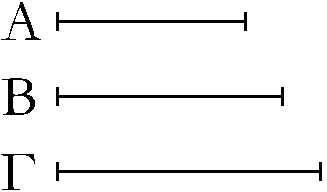
\includegraphics{Book09/fig16g.pdf}}

\gr{Δύο γὰρ ἀριθμοὶ οἱ Α, Β πρῶτοι πρὸξ ἀλλήλουξ >έστωσαν; λέγω,
<ότι οὐκ >έστιν ὡξ ὁ Α πρὸξ τὸν Β, ο<ύτωξ ὁ Β πρὸξ >άλλον
τινά.}

\gr{Εἰ γὰρ δυνατόν, >έστω ὡξ ὁ Α πρὸξ τὸν Β, ὁ Β πρὸξ τὸν Γ.
οἱ δὲ Α, Β πρῶτοι, οἱ δὲ πρῶτοι καὶ ἐλάθιστοι, οἱ δὲ ἐλάθιστοι
ἀριθμοὶ μετροῦσι τοὺξ τὸν α\kern -.7pt  ὐτὸν λόγον >έθονταξ ἰσάκιξ
<ό τε ἡγούμενοξ τὸν ἡγούμενον καὶ ὁ ἑπόμενοξ τὸν ἑπόμενον;
μετρεῖ >άρα ὁ Α τὸν Β ὡξ ἡγούμενοξ ἡγούμενον.
μετρεῖ δὲ καὶ ἑαυτόν; ὁ Α >άρα τοὺξ Α, Β
μετρεῖ πρώτουξ >όνταξ πρὸξ ἀλλήλουξ; <όπερ >άτοπον. οὐκ >άρα
>έσται ὡξ ὁ Α πρὸξ τὸν Β, ο<ύτωξ ὁ Β πρὸξ τὸν Γ; <όπερ
>έδει δεῖχαι.}}

\ParallelRText{
\begin{center}
{\large Proposition 16}
\end{center}

If two numbers are prime to one another then as the
first is to the second, so the second (will) not (be) to some other (number).

% Removed epsf size command
\centerline{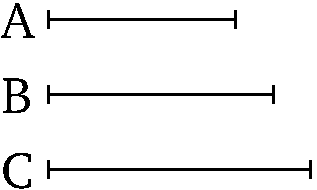
\includegraphics{Book09/fig16e.pdf}}

For let the two numbers $A$ and $B$ be prime to one another. I say that
as $A$ is to $B$, so $B$ is not to some other (number).

For, if possible, let it be that as $A$ (is) to $B$, (so) $B$ (is) to $C$. And $A$ and $B$
(are) prime (to one another). And (numbers) prime (to one another are)
also the least (of those numbers having the same ratio as them) [Prop.~7.21]. And the least numbers measure those
(numbers) having the same ratio (as them) an equal number of times,
the leading (measuring) the leading, and the following the following [Prop.~7.20]. Thus, $A$ measures $B$, 
as the leading (measuring) the leading. And ($A$) also measures itself.
Thus, $A$ measures $A$ and $B$, which are prime to one another. The very
thing (is) absurd. Thus, as $A$  (is) to $B$, so $B$ cannot be to $C$.
(Which is) the very thing it was required to show.}
\end{Parallel}

%%%%%%
% Prop 9.17
%%%%%%
\pdfbookmark[1]{Proposition 9.17}{pdf9.17}
\begin{Parallel}{}{} 
\ParallelLText{
\begin{center}
{\large \ggn{17}.}
\end{center}\vspace*{-7pt}

\gr{Ἐὰν >ῶσιν ὁσοιδηποτοῦν ἀριθμοὶ ἑχῆξ ἀνάλογον, οἱ δὲ >άκροι
α\kern -.7pt  ὐτῶν πρῶτοι πρὸξ ἀλλήλουξ >ῶσιν, οὐκ >έσται ὡξ ὁ πρῶτοξ
πρὸξ τὸν δεύτερον, ο<ύτωξ ὁ >έσθατοξ πρὸξ >άλλον τινά.}

\gr{>'Εστωσαν ὁσοιδηποτοῦν ἀριθμοὶ ἑχῆξ ἀνάλογον οἱ Α, Β, Γ, Δ,
οἱ δὲ >άκροι α\kern -.7pt  ὐτῶν οἱ Α, Δ πρῶτοι πρὸξ ἀλλήλουξ >έστωσαν;
λέγω, <ότι οὐκ >έστιν ὡξ ὁ Α πρὸξ τὸν Β, ο<ύτωξ ὁ Δ πρὸξ >άλλον
τινά.}\\

% Removed epsf size command
\centerline{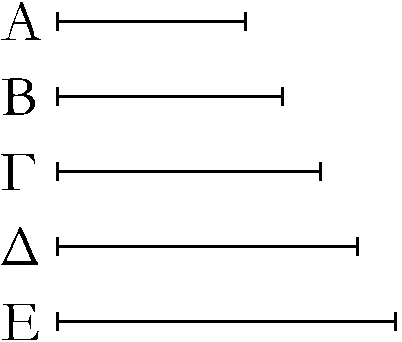
\includegraphics{Book09/fig17g.pdf}}

\gr{Εἰ  γὰρ δυνατόν, >έστω ὡξ ὁ Α πρὸξ τὸν Β, ο<ύτωξ
ὁ Δ πρὸξ τὸν Ε; ἐναλλὰχ >άρα ἐστὶν ὡξ ὁ Α πρὸξ τὸν Δ, ὁ Β πρὸξ τὸν Ε. οἱ δὲ Α, Δ πρῶτοι, οἱ δὲ πρῶτοι καὶ ἐλάθιστοι, οἱ δὲ
ἐλάθιστοι ἀριθμοὶ μετροῦσι τοὺξ τὸν α\kern -.7pt  ὐτὸν λόγον >έθονταξ
ἰσάκιξ <ό τε ἡγούμενοξ τὸν ἡγούμενον καὶ ὁ ἑπόμενοξ
τὸν ἑπόμενον. μετρεῖ >άρα ὁ Α τὸν Β. καί ἐστιν ὡξ ὁ Α
πρὸξ τὸν Β, ὁ Β πρὸξ τὸν Γ. καὶ ὁ Β >άρα τὸν Γ μετρεῖ';
<ώστε καὶ ὁ Α τὸν Γ μετρεῖ. καὶ ἐπεί ἐστιν ὡξ ὁ Β πρὸξ
τὸν Γ, ὁ Γ πρὸξ τὸν Δ, μετρεῖ δὲ ὁ Β τὸν Γ, μετρεῖ >άρα καὶ
ὁ Γ τὸν Δ. ἀλλ> ὁ Α τὸν Γ
ἐμέτρει; <ώστε
ὁ Α καὶ τὸν Δ μετρεῖ. μετρεῖ δὲ καὶ ἑαυτόν. ὁ Α >άρα τοὺξ
Α, Δ μετρεῖ πρώτουξ >όνταξ πρὸξ ἀλλήλουξ; <όπερ ἐστὶν ἀδύνατον.
οὐκ >άρα >έσται ὡξ ὁ Α πρὸξ τὸν Β, ο<ύτωξ ὁ Δ πρὸξ >άλλον
τινά; <όπερ >έδει δεῖχαι.}}

\ParallelRText{
\begin{center}
{\large Proposition 17}
\end{center}

If   any multitude whatsoever of numbers is continuously proportional, and the outermost of them are prime to one another, then as the first (is) to the second, so the last will not be
to some other (number).

Let $A$, $B$, $C$, $D$ be any multitude whatsoever of continuously
proportional numbers. And let the outermost of them, $A$ and $D$,
be prime to one another. I say that as $A$ is to $B$, so $D$ (is) not to some
other (number).

% Removed epsf size command
\centerline{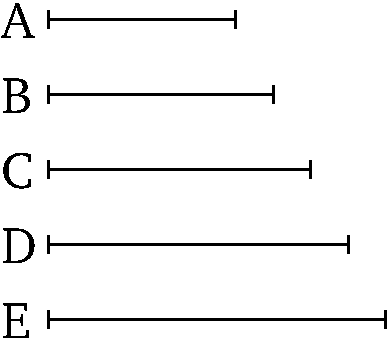
\includegraphics{Book09/fig17e.pdf}}

For, if possible, let it be that as $A$ (is) to $B$, so $D$ (is) to $E$. 
Thus, alternately, as $A$ is to $D$, (so) $B$ (is) to $E$ [Prop.~7.13]. And $A$ and $D$ are prime (to one another).  And (numbers) prime (to one another are)
also the least (of those numbers having the same ratio as them) [Prop.~7.21]. And the least numbers measure those
(numbers) having the same ratio (as them) an equal number of times,
the leading (measuring) the leading, and the following the following [Prop.~7.20]. Thus, $A$ measures $B$. And as $A$
is to $B$, (so) $B$ (is) to $C$.  Thus, $B$ also measures $C$.  And hence
$A$ measures $C$ [Def.~7.20]. And since as $B$ is to
$C$, (so) $C$ (is) to $D$, and $B$ measures $C$, $C$ thus also measures
$D$ [Def.~7.20].  But, $A$ was (found to be) measuring $C$. And 
hence $A$ also measures $D$. And ($A$) also measures itself.  Thus, $A$
measures $A$ and $D$, which are prime to one another. The very thing is impossible. Thus, as $A$ (is) to $B$, so $D$ cannot be to some other (number). (Which is) the very thing it was required to show.}
\end{Parallel}

%%%%%%
% Prop 9.18
%%%%%%
\pdfbookmark[1]{Proposition 9.18}{pdf9.18}
\begin{Parallel}{}{} 
\ParallelLText{
\begin{center}
{\large \ggn{18}.}
\end{center}\vspace*{-7pt}

\gr{Δύο ἀριθμῶν δοθέντων ἐπισκέψασθαι, εἰ δυνατόν ἐστιν α\kern -.7pt  ὐτοῖξ
τρίτον ἀνάλογον προσευρεῖν.}

% Removed epsf size command
\centerline{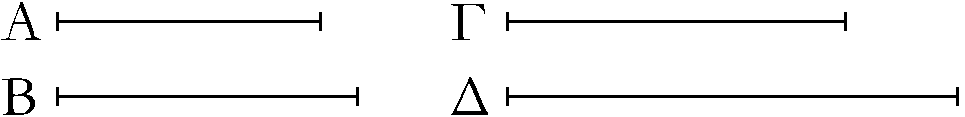
\includegraphics{Book09/fig18g.pdf}}

\gr{>'Εστωσαν οἱ δοθέντεξ δύο ἀριθμοὶ οἱ Α, Β, καὶ δέον >έστω ἐπισκέψασθαι, εἰ δυνατόν ἐστιν α\kern -.7pt  ὐτοῖξ τρίτον ἀνάλογον προσευρεῖν.}

\gr{Οἱ  δὴ Α, Β >ήτοι πρῶτοι πρὸξ ἀλλήλουξ εἰσὶν >ὴ
ο>ύ. καὶ εἰ πρῶτοι πρὸξ ἀλλήλουξ εἰσίν, δέδεικται, <ότι
ἀδύνατόν ἐστιν α\kern -.7pt  ὐτοῖξ τρίτον ἀνάλογον προσευρεῖν.}

\gr{Ἀλλὰ δὴ μ\kern -.7pt  ὴ >έστωσαν οἱ Α, Β πρῶτοι πρὸξ ἀλλήλουξ, καὶ ὁ Β ἑαυτον
πολλαπλασιάσαξ τὸν Γ ποιείτω. ὁ Α δὴ τὸν Γ >ήτοι μετρεῖ >ὴ οὐ
μετρεῖ. μετρείτω πρότερον κατὰ τὸν Δ; ὁ Α >άρα τὸν Δ πολλαπλασιάσαξ
τὸν Γ πεποίηκεν. ἀλλα μ\kern -.7pt  ὴν καὶ ὁ Β ἑαυτὸν πολλαπλασιάσαξ τὸν Γ
πεποίηκεν; ὁ >άρα ἐκ τῶν Α, Δ >ίσοξ ἐστὶ τῶ| ἀπὸ τοῦ Β. >έστιν
>άρα ὡξ ὁ Α πρὸξ τὸν Β, ὁ Β πρὸξ τὸν Δ; τοῖξ Α, Β >άρα τρίτοξ
ἀριθμὸξ ἀνάλογον προσηύρηται ὁ Δ.}

\gr{Ἀλλὰ δὴ μ\kern -.7pt  ὴ μετρείτω ὁ Α τὸν Γ; λέγω, <ότι τοῖξ Α, Β ἀδύνατόν ἐστι
τρίτον ἀνάλογον προσευρεῖν ἀριθμόν. εἰ γὰρ δυνατόν, προσηυρήσθω
ὁ Δ. ὁ >άρα ἐκ τῶν Α, Δ >ίσοξ ἐστὶ τῶ| ἀπὸ τοῦ Β. ὁ δὲ
ἀπὸ τοῦ Β ἐστιν ὁ Γ; ὁ >άρα ἐκ τῶν
Α, Δ >ίσοξ ἐστὶ τῶ| Γ. <ώστε ὁ Α τὸν Δ πολλαπλασιάσαξ τὸν Γ 
πεποίηκεν; ὁ Α >άρα τὸν Γ μετρεῖ κατὰ τὸν Δ. ἀλλα μ\kern -.7pt  ὴν ὑπόκειται
καὶ μ\kern -.5pt  ὴ μετρῶν; <όπερ >άτοπον. οὐκ >άρα δυνατόν ἐστι
τοῖξ Α, Β τρίτον ἀνάλογον προσευρεῖν ἀριθμὸν, <όταν ὁ Α τὸν Γ μ\kern -.3pt  ὴ
μετρῆ|; <όπερ >έδει δεῖχαι.}}

\ParallelRText{
\begin{center}
{\large Proposition 18}
\end{center}

For  two given numbers, to investigate whether it
is possible to find a third (number) proportional to them.

% Removed epsf size command
\centerline{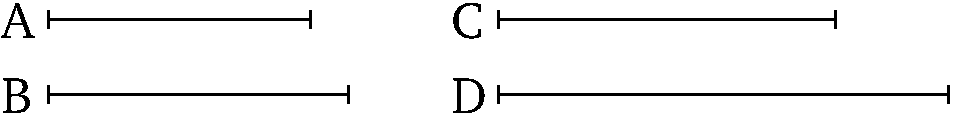
\includegraphics{Book09/fig18e.pdf}}

Let $A$ and $B$ be the two given numbers. And let it be required to investigate whether it is possible to find a third (number) proportional
to them.

So $A$ and $B$ are either prime to one another, or not. 
And if they are prime to one another then it has (already) been show that it is impossible
to find a third (number) proportional to them [Prop.~9.16].

And so let $A$ and $B$ not be prime to one another. And let $B$ make $C$
(by) multiplying itself. So $A$ either measures, or does not measure, $C$. 
Let it first of all measure ($C$) according to $D$. Thus, $A$ has made
$C$ (by) multiplying $D$. But, in fact, $B$ has also made
$C$ (by) multiplying itself. Thus, the (number created) from (multiplying)
$A$, $D$ is equal to the (square) on $B$. Thus, as $A$ is to $B$, (so)
$B$ (is) to $D$ [Prop.~7.19]. Thus, a third number
has been found proportional to $A$, $B$, (namely) $D$. 

And so let $A$ not measure $C$. I say that it is impossible to find a third
number proportional to $A$, $B$. For, if possible, let it be found,
(and let it be) $D$. Thus, the (number created) from (multiplying) $A$, $D$
is equal to the (square) on $B$ [Prop.~7.19]. 
And the (square) on $B$ is $C$. Thus, the (number created) from (multiplying) $A$, $D$
is equal to $C$. Hence, $A$ has made $C$ (by) multiplying $D$. 
Thus, $A$ measures $C$ according to $D$. But ($A$) was, in fact, also assumed
(to be) not measuring ($C$). The very thing (is) absurd. Thus, it is not
possible to find a third number proportional to $A$, $B$ when $A$ does not
measure $C$. (Which is) the very thing it was required to show.}
\end{Parallel}

%%%%%%
% Prop 9.19
%%%%%%
\pdfbookmark[1]{Proposition 9.19}{pdf9.19}
\begin{Parallel}{}{} 
\ParallelLText{
\begin{center}
{\large \ggn{19}.}
\end{center}\vspace*{-7pt}

\gr{Τριῶν ἀριθμῶν δοθέντων ἐπισκέψασθαι, πότε δυνατόν ἐστιν α\kern -.7pt  ὐτοῖξ
τέταρτον ἀνάλογον προσευρεῖν.}

% Removed epsf size command
\centerline{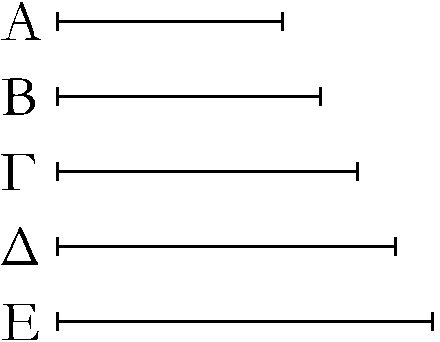
\includegraphics{Book09/fig19g.pdf}}

\gr{>'Εστωσαν οἱ δοθέντεξ τρεῖξ ἀριθμοὶ οἱ Α, Β, Γ, καὶ δέον >έστω
επισκέψασθαι, πότε δυνατόν ἐστιν α\kern -.7pt  ὐτοῖξ τέταρτον
ἀνάλογον προσευρεῖν.}

\gr{>'Ητοι ο>ῦν ο>ύκ εἰσιν ἑχῆξ ἀνάλογον, καὶ οἱ >άκροι α\kern -.7pt  ὐτῶν πρῶτοι
πρὸξ ἀλλήλουξ εἰσίν, >ὴ ἑχῆξ εἰσιν ἀνάλογον, καὶ οἱ
>άκροι α\kern -.7pt  ὐτῶν ο>ύκ εἰσι πρῶτοι πρὸξ ἀλλήλουξ, >ὴ ο<ύτε
ἑχῆξ εἰσιν ἀνάλογον, ο>ύτε οἱ >άκροι α\kern -.5pt  ὐτῶν πρῶτοι
πρὸξ ἀλλήλουξ εἰσίν, >ὴ καὶ ἑχῆξ εἰσιν ἀνάλογον, καὶ
οἱ >άκροι α\kern -.3pt  ὐτῶν πρῶτοι πρὸξ ἀλλήλουξ εἰσίν.}

\gr{Εἰ μὲν ο>ῦν οἱ Α, Β, Γ ἑχῆξ εἰσιν ἀνάλογον, καὶ οἱ >άκροι
α\kern -.7pt  ὐτῶν οἱ Α, Γ πρῶτοι πρὸξ ἀλλήλουξ εἰσίν, δέδεικται, <ότι
ἀδύνατόν ἐστιν α\kern -.7pt  ὐτοῖξ τέταρτον ἀνάλογον προσευρεῖν ἀριθμόν. μ\kern -.5pt  ὴ
>έστωσαν δὴ οἱ Α, Β, Γ ἑχῆξ ἀνάλογον τῶν ἀκρῶν πάλιν
>όντων πρώτων πρὸξ  ἀλλήλουξ. λέγω, <ότι καὶ ο<ύτωξ ἀδύνατόν ἐστιν
α\kern -.3pt  ὐτοῖξ τέταρτον ἀνάλογον προσευρεῖν. εἰ γὰρ δυνατόν, προσευρήσθω
ὁ Δ, <ώστε ε>ῖναι ὡξ τὸν Α πρὸξ τὸν Β, τὸν Γ πρὸξ τὸν Δ, καὶ
γεγονέτω ὡξ ὁ Β πρὸξ τὸν Γ, ὁ Δ πρὸξ τὸν Ε. καὶ ἐπεί ἐστιν ὡξ μὲν ὁ Α πρὸξ τὸν Β, ὁ Γ πρὸξ τὸν Δ, ὡξ  δὲ ὁ Β πρὸξ τὸν 
Γ, ὁ Δ πρὸξ τὸν Ε, δι> >ίσου >άρα ὡξ ὁ Α πρὸξ τὸν Γ, ὁ Γ πρὸξ τὸν Ε. οἱ δὲ Α, Γ πρῶτοι, οἱ δὲ
πρῶτοι καὶ ἐλάθιστοι, οἱ δὲ ἐλάθιστοι μετροῦσι τοὺξ τὸν α\kern -.7pt  ὐτὸν
λόγον >έθονταξ <ό τε ἡγούμενοξ τὸν ἡγούμενον
καὶ ὁ ἑπόμενοξ τὸν ἑπόμενον. μετρεῖ >άρα ὁ Α τὸν Γ ὡξ
ἡγούμενοξ ἡγούμενον. μετρεῖ δὲ καὶ ἑαυτόν;
ὁ Α >άρα τοὺξ Α, Γ μετρεῖ πρώτουξ >όνταξ πρὸξ ἀλλήλουξ; <όπερ
ἐστὶν ἀδύνατον. οὐκ >άρα τοῖξ Α, Β, Γ δυνατόν ἐστι τέταρτον
ἀνάλογον προσευρεῖν.}

\gr{Ἀλλά δὴ πάλιν >έστωσαν οἱ Α, Β, Γ ἑχῆξ ἀνάλογον, οἱ δὲ Α, Γ μ\kern -.7pt  ὴ
>έστωσαν πρῶτοι πρὸξ ἀλλήλουξ. λέγω, <ότι δυνατόν ἐστιν α\kern -.7pt  ὐτοῖξ τέταρτον ἀνάλογον προσευρεῖν. ὁ γὰρ Β τὸν Γ πολλαπλασιάσαξ
τὸν Δ ποιείτω; ὁ Α >άρα τὸν Δ >ήτοι μετρεῖ >ὴ οὐ μετρεῖ. μετρείτω
α\kern -.5pt  ὐτὸν πρότερον κατὰ τὸν Ε; ὁ Α >άρα τὸν Ε πολλαπλασιάσαξ τὸν Δ
πεποίηκεν. ἀλλὰ μ\kern -.3pt  ὴν καὶ ὁ Β τὸν Γ  πολλαπλασιάσαξ τὸν Δ πεποίηκεν;
ὁ >άρα ἐκ τῶν Α, Ε >ίσοξ ἐστὶ τῶ| ἐκ τῶν Β, Γ. ἀνάλογον
>άρα [ἐστὶν] ὡξ ὁ Α πρὸξ τὸν Β, ὁ Γ πρὸξ τὸν Ε; τοὶξ Α, Β, Γ
>άρα τέταρτοξ ἀνάλογον προσηύρηται ὁ Ε.}

\gr{Ἀλλὰ δὴ μ\kern -.7pt  ὴ μετρείτω ὁ Α τὸν Δ; λέγω, <ότι ἀδύνατόν ἐστι τοῖξ
Α, Β, Γ τέταρτον ἀνάλογον προσευρεῖν ἀριθμόν. εἰ γὰρ δυνατόν,
προσευρήσθω ὁ Ε; ὁ >άρα ἐκ τῶν Α, Ε >ίσοξ ἐστὶ τῶ| ἐκ τῶν Β, Γ.
ἀλλὰ ὁ ἑκ τῶν Β, Γ ἐστιν ὁ Δ; καὶ ὁ ἐκ τῶν Α, Ε >άρα >ίσοξ ἐστὶ τῶ| Δ. ὁ Α >άρα τὸν Ε πολλαπλασιάσαξ τὸν Δ πεποίηκεν; ὁ Α
>άρα τὸν Δ μετρεῖ κατὰ τὸν  Ε; <ώστε μετρεῖ ὁ Α τὸν Δ. ἀλλὰ
καὶ οὐ μετρεῖ; <όπερ >άτοπον. οὐκ >άρα δυνάτον ἐστι τοῖξ
Α, Β, Γ τέταρτον ἀνάλογον προσευρεῖν ἀριθμόν, <όταν ὁ Α τὸν
Δ μ\kern -.7pt  ὴ μετρῆ|. ἀλλὰ δὴ οἱ Α, Β, Γ μ\kern -.5pt  ήτε ἑχῆξ >έστωσαν ἀνάλογον
μ\kern -.3pt  ήτε οἱ >άκροι πρῶτοι πρὸξ ἀλλήλουξ. καὶ ὁ Β τὸν Γ πολλαπλασιάσαξ
τὸν Δ ποιείτω. ὁμοίωξ δὴ δειθθήσεται, <ότι εἰ μὲν μετρεῖ ὁ Α τὸν Δ,
δυνατόν ἐστιν α\kern -.7pt  ὐτοῖξ ἀνάλογον προσευρεῖν, εἰ δὲ οὐ μετρεῖ,
ἀδύνατον; <όπερ >έδει δεῖχαι.}}

\ParallelRText{
\begin{center}
{\large Proposition 19}$^\dag$
\end{center}

For three given numbers, to investigate when it is
possible to find a fourth (number) proportional to them.

% Removed epsf size command
\centerline{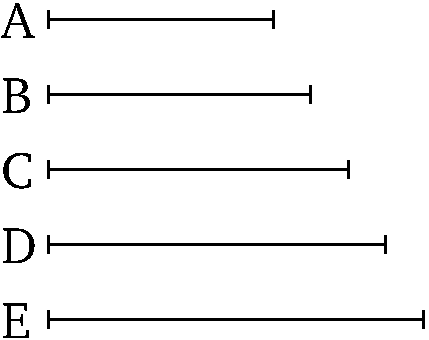
\includegraphics{Book09/fig19e.pdf}}

Let $A$, $B$, $C$ be the three given numbers. And let it be required to
investigate when it is possible to find a fourth (number) proportional to them.

In fact, ($A$, $B$, $C$) are either not continuously proportional and the outermost
of them are prime to one another, or are continuously proportional
and the outermost of them are not prime to one another, or are neither
continuously proportional nor are the outermost of them prime to one another, or are continuously proportional and the outermost of them are
prime to one another.

In fact, if $A$, $B$, $C$ are continuously proportional, and the outermost
of them, $A$ and $C$, are prime to one another, (then) it has (already) been shown that it is impossible to find a fourth number proportional to them
[Prop.~9.17]. So let $A$, $B$, $C$
not be continuously proportional, (with) the outermost of them again being
prime to one another. I say that, in this case, it is also impossible to find a fourth (number)
proportional to them. For, if possible, let it be found,
(and let it be) $D$. Hence, it will be that as $A$ (is) to $B$, (so)
$C$ (is) to $D$. And let it be contrived that as $B$ (is) to $C$, (so) $D$ (is) to $E$. And since as $A$ is to $B$, (so) $C$ (is) to $D$, and as $B$ (is) to $C$, (so)
$D$ (is) to $E$, thus, via equality, as $A$ (is) to $C$, (so) $C$ (is) to $E$
[Prop.~7.14]. And $A$ and $C$ (are) prime (to one another). And (numbers) prime (to one another are) also the least (numbers
having the same ratio as them) [Prop.~7.21]. 
And the least (numbers) measure those numbers having the same ratio
as them (the same number of times), the leading (measuring) the leading,
and the following the following [Prop.~7.20]. 
Thus, $A$ measures $C$, (as) the leading (measuring) the leading.
And it also measures itself. Thus, $A$ measures $A$ and $C$, which are
prime to one another. The very thing is impossible. Thus, it is not possible to find a fourth (number) proportional to $A$, $B$, $C$.

And so let $A$, $B$, $C$  again be continuously proportional, and let $A$ and $C$ not be prime to one another. I say that it is possible to find
a fourth (number) proportional to them. For let $B$ make $D$ (by) multiplying $C$. Thus, $A$ either measures or does not measure $D$. 
Let it, first of all, measure ($D$) according to $E$. Thus, $A$ has made $D$ (by) multiplying $E$. But, in fact, $B$ has also made $D$ (by) multiplying $C$. Thus, the (number created) from (multiplying) $A$, $E$
is equal to the (number created) from (multiplying) $B$, $C$. Thus, 
proportionally, as $A$ [is] to $B$, (so) $C$ (is) to $E$ [Prop.~7.19]. Thus, a fourth (number) proportional
to $A$, $B$, $C$ has been found, (namely) $E$.

And so let $A$ not measure $D$. I say that it is impossible to find a fourth
number proportional to $A$, $B$, $C$. For, if possible, let it 
be found, (and let it be) $E$. Thus, the (number created) from
(multiplying) $A$, $E$ is equal to the (number created) from (multiplying)
$B$, $C$. But, the (number created) from (multiplying) $B$, $C$ is $D$.
And thus the (number created) from (multiplying) $A$, $E$ is equal to $D$.
Thus, $A$ has made $D$ (by) multiplying $E$. Thus, $A$ measures
$D$ according to $E$. Hence, $A$ measures $D$. But, it also does not
measure ($D$). The very thing (is) absurd. Thus, it is not possible
to find a fourth number proportional to $A$, $B$, $C$ when $A$ does not
measure $D$. And so (let) $A$, $B$, $C$ (be) neither continuously
proportional, nor (let) the outermost of them (be) prime to one another.
And let $B$ make $D$ (by) multiplying $C$. So, similarly, it can be show that
if $A$ measures $D$ then it is possible to find a fourth (number)
proportional to ($A$, $B$, $C$), and impossible if ($A$) does not measure ($D$).
(Which is) the very thing it was required to show.}
\end{Parallel}
{\footnotesize\noindent$^\dag$ The proof of this proposition is incorrect.
There are, in fact, only two cases. Either $A$, $B$, $C$ are continuously
proportional,  with $A$ and $C$ prime to one another, or not. In the first case, 
it is impossible to find a fourth proportional number. In the second case,
it is possible to find a fourth proportional number provided that $A$
measures $B$ times $C$. Of the four cases considered by Euclid,
the proof given in the second case is incorrect, since it only demonstrates that
if $A:B::C:D$ then a number $E$ cannot be found such that $B:C::D:E$. The proofs given in the other three cases are correct.}

%%%%%%
% Prop 9.20
%%%%%%
\pdfbookmark[1]{Proposition 9.20}{pdf9.20}
\begin{Parallel}{}{} 
\ParallelLText{
\begin{center}
{\large\ggn{20}.}
\end{center}\vspace*{-7pt}

\gr{Οἱ πρῶτοι ἀριθμοὶ πλείουξ εἰσὶ παντὸξ τοῦ προτεθέντοξ πλήθουξ
πρώτων ἀριθμῶν.}

% Removed epsf size command
\centerline{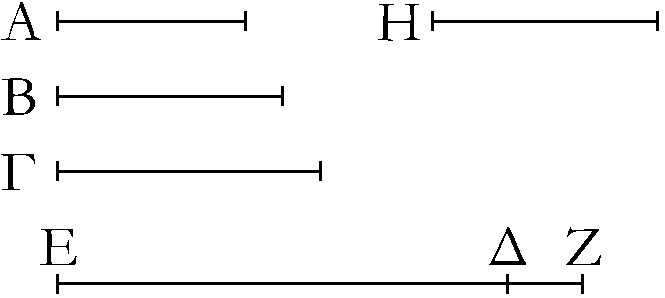
\includegraphics{Book09/fig20g.pdf}}

\gr{>'Εστωσαν οἱ προτεθέντεξ πρῶτοι ἀριθμοὶ οἱ Α, Β, Γ; λέγω,
<ότι τῶν Α, Β, Γ πλείουξ εἰσὶ πρῶτοι ἀριθμοί.}

\gr{Εἰλήφθω γὰρ ὁ ὑπὸ τῶν Α, Β, Γ ἐλάθιστοξ μετρούμενοξ καὶ >έστω
ΔΕ, καὶ προσκείσθω τῶ| ΔΕ μονὰξ ἡ ΔΖ. ὁ δὴ ΕΖ >ήτοι πρῶτόξ
ἐστιν >ὴ ο>ύ. >έστω πρότερον πρῶτοξ; εὐρημένοι >άρα εἰσὶ πρῶτοι
ἀριθμοὶ οἱ Α, Β, Γ, ΕΖ πλείουξ τῶν Α, Β, Γ.}

\gr{Ἀλλὰ δὴ μ\kern -.7pt  ὴ >έστω ὁ ΕΖ πρῶτοξ; ὑπὸ πρώτου
>άρα τινὸξ ἀριθμοῦ μετρεῖται. μετρείσθω ὑπὸ πρώτου τοῦ Η;
λέγω, <ότι ὁ Η οὐδενὶ τῶν Α, Β, Γ ἐστιν ὁ α\kern -.7pt  ὐτόξ. εἰ γὰρ
δυνατόν, >έστω. οἱ δὲ Α, Β, Γ τὸν ΔΕ μετροῦσιν; καὶ ὁ Η >άρα
τὸν ΔΕ μετρήσει. μετρεῖ δὲ καὶ τὸν ΕΖ; καὶ λοιπὴν τὴν ΔΖ μονάδα
μετρήσει ὁ Η ἀριθμὸξ >ών; >όπερ >άτοπον. οὐκ >άρα ὁ
Η ἑνὶ τῶν Α, Β, Γ ἐστιν ὁ α\kern -.5pt  ὐτόξ. καὶ ὑπόκειται πρῶτοξ.
εὑρημένοι >άρα εἰσὶ πρῶτοι ἀριθμοὶ πλείουξ
τοῦ προτεθέντοξ πλήθουξ τῶν Α, Β, Γ οἱ Α, Β, Γ, Η;
<όπερ >έδει δεῖχαι.}}

\ParallelRText{
\begin{center}
{\large Proposition 20}
\end{center}

The (set of all) prime numbers is more numerous than any assigned
multitude of prime numbers.

% Removed epsf size command
\centerline{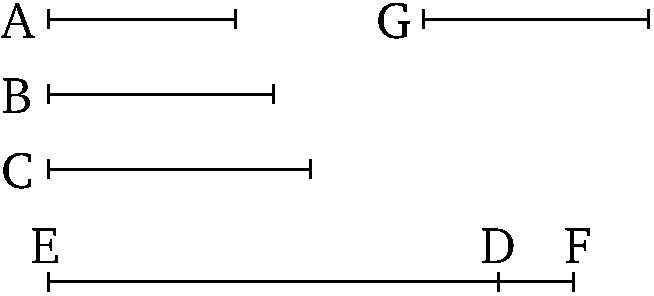
\includegraphics{Book09/fig20e.pdf}}

Let $A$, $B$, $C$ be the assigned prime numbers. I say that the (set of all)
primes numbers is more numerous than $A$, $B$, $C$.

For let the least number measured by  $A$, $B$, $C$ be taken, and let it be $DE$ [Prop.~7.36]. And let the unit $DF$ be added to $DE$. So $EF$ is either prime, or not. Let it, first of all,
be prime. Thus, the (set of) prime numbers $A$, $B$, $C$, $EF$, (which is) more numerous than $A$, $B$, $C$, has been found.

And so let $EF$ not be prime. Thus, it is measured by some prime number [Prop.~7.31]. Let it be measured by the prime
(number) $G$. I say that $G$ is not the same as any of $A$, $B$, $C$. 
For, if possible, let it be (the same). And $A$, $B$, $C$ (all) measure
$DE$. Thus, $G$ will also measure $DE$. And it also measures $EF$. (So)
$G$ will also measure the remainder, unit $DF$, (despite) being a number
[Prop.~7.28]. The very thing (is) absurd. Thus, $G$
is not the same as one of $A$, $B$, $C$. And it was assumed (to be) prime.
Thus, the (set of) prime numbers $A$, $B$, $C$, $G$, (which is) more numerous than the assigned multitude (of prime numbers), $A$, $B$, $C$, has been found. (Which is) the very thing it
was required to show.}
\end{Parallel}

%%%%%%
% Prop 9.21
%%%%%%
\pdfbookmark[1]{Proposition 9.21}{pdf9.21}
\begin{Parallel}{}{} 
\ParallelLText{
\begin{center}
{\large \ggn{21}.}
\end{center}\vspace*{-7pt}

\gr{Ἐὰν >άρτιοι ἀριθμοὶ ὁποσοιοῦν συντεθῶσιν, ὁ <όλοξ >άρτιόξ
ἐστιν.}

% Removed epsf size command
\centerline{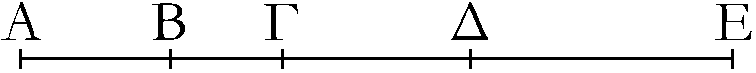
\includegraphics{Book09/fig21g.pdf}}

\gr{Συγκείσθωσαν γὰρ >άρτιοι ἀριθμοὶ ὁποσοιοῦν οἱ ΑΒ, ΒΓ, ΓΔ, ΔΕ;
λέγω, <ότι <όλοξ ὁ ΑΕ >άρτιόξ ἐστιν.}

\gr{Ἐπεὶ γὰρ <έκαστοξ τῶν ΑΒ, ΒΓ, ΓΔ, ΔΕ >άρτιόξ ἐστιν, >έθει
μέροξ <ήμισυ; <ώστε καὶ <όλοξ ὁ ΑΕ >έθει μέροξ <ήμισυ.
>άρτιοξ δὲ ἀριθμόξ ἐστιν ὁ δίθα διαιρούμενοξ;
>άρτιοξ >άρα ἐστὶν ὁ ΑΕ; <όπερ >έδει δεῖχαι.}}

\ParallelRText{
\begin{center}
{\large Proposition 21}
\end{center}

If any multitude whatsoever of even numbers
is added together then the whole is even.

% Removed epsf size command
\centerline{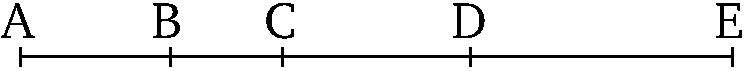
\includegraphics{Book09/fig21e.pdf}}

For let any multitude  whatsoever of even numbers, $AB$, $BC$, $CD$, $DE$, lie together. I say that the whole, $AE$, is even.

For since everyone  of $AB$, $BC$, $CD$, $DE$ is even, it has a half part
[Def.~7.6]. And hence the whole $AE$ has
a half part. And an even number is one (which can be) divided in half [Def.~7.6]. Thus, $AE$ is even. (Which is) the very thing it was required to show.}
\end{Parallel}

%%%%%%
% Prop 9.22
%%%%%%
\pdfbookmark[1]{Proposition 9.22}{pdf9.22}
\begin{Parallel}{}{} 
\ParallelLText{
\begin{center}
{\large \ggn{22}.}
\end{center}\vspace*{-7pt}

\gr{Ἐὰν περισσοὶ ἀριθμοὶ ὁποσοιοῦν συντεθῶσιν, τὸ δὲ πλῆθοξ
α\kern -.7pt  ὐτῶν >άρτιον >ῆ|, ὁ <όλοξ >άρτιοξ >έσται.}\\

% Removed epsf size command
\centerline{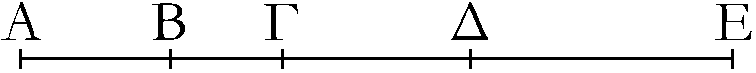
\includegraphics{Book09/fig21g.pdf}}

\gr{Συγκείσθωσαν γὰρ περισσοὶ ἀριθμοὶ ὁσοιδηποτοῦν >άρτιοι
τὸ πλῆθοξ οἱ ΑΒ, ΒΓ, ΓΔ, ΔΕ; λέγω, <ότι <όλοξ ὁ ΑΕ >άρτιόξ
ἐστιν.}

\gr{Ἐπεὶ γὰρ <έκαστοξ τῶν ΑΒ, ΒΓ, ΓΔ, ΔΕ περιττόξ ἐστιν, ἀφαιρεθείσηξ
μονάδοξ ἀφ> ἑκάστου <έκαστοξ τῶν λοιπῶν >άρτιοξ >έσται; <ώστε
καὶ ὁ συγκείμενοξ ἐχ α\kern -.7pt  ὐτῶν >άρτιοξ >έσται. >έστι δὲ καὶ τὸ
πλῆθοξ τῶν μονάδων >άρτιον. καὶ <όλοξ >άρα ὁ ΑΕ >άρτιόξ
ἐστιν; <όπερ >έδει δεῖχαι.}}

\ParallelRText{
\begin{center}
{\large Proposition 22}
\end{center}

If any multitude whatsoever of odd numbers
is added together, and the multitude of them is even,  then the whole will be even.

% Removed epsf size command
\centerline{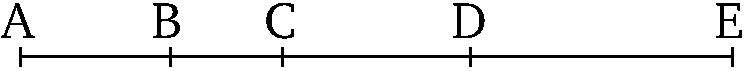
\includegraphics{Book09/fig21e.pdf}}

For let any even multitude whatsoever of odd numbers, 
$AB$, $BC$, $CD$, $DE$, lie together. I say that the whole, $AE$, is even.

For since everyone of $AB$, $BC$, $CD$, $DE$ is odd then,  a unit being subtracted from
each, everyone of the remainders will be (made) even [Def.~7.7]. And hence the sum of them will be even [Prop.~9.21]. And the multitude  of the units is even.
Thus, the whole $AE$ is also even [Prop.~9.21]. (Which is) the very thing it was required to show.}
\end{Parallel}

%%%%%%
% Prop 9.23
%%%%%%
\pdfbookmark[1]{Proposition 9.23}{pdf9.23}
\begin{Parallel}{}{} 
\ParallelLText{
\begin{center}
{\large\ggn{23}.}
\end{center}\vspace*{-7pt}

\gr{Ἐὰν περισσοὶ ἀριθμοὶ ὁποσοιοῦν συντεθῶσιν, τὸ
δὲ πλῆθοξ α\kern -.7pt  ὐτῶν περισσὸν >ῆ|, καὶ ὁ <όλοξ περισσὸξ >έσται.}\\

% Removed epsf size command
\centerline{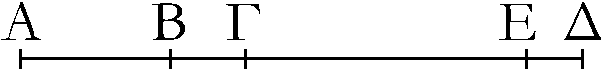
\includegraphics{Book09/fig23g.pdf}}

\gr{Συγκείσθωσαν γὰρ ὁποσοιοῦν περισσοὶ ἀριθμοί, <ῶν τὸ πλῆθοξ
περισσὸν >έστω, οἱ ΑΒ, ΒΓ, ΓΔ; λέγω, <ότι καὶ <όλοξ ὁ ΑΔ περισσόξ
ἐστιν.}

\gr{Ἀφῃρήσθω ἀπὸ τοῦ ΓΔ μονὰξ ἡ ΔΕ; λοιπὸξ >άρα ὁ ΓΕ >άρτιόξ
ἐστιν. >έστι δὲ καὶ ὁ ΓΑ >άρτιοξ; καὶ <όλοξ >άρα ὁ ΑΕ >άρτιόξ 
ἐστιν. καί ἐστι μονὰξ ἡ ΔΕ. περισσὸξ >άρα ἐστὶν ὁ ΑΔ; <όπερ
>έδει δεῖχαι.}}

\ParallelRText{
\begin{center}
{\large Proposition 23}
\end{center}

If  any multitude whatsoever of odd numbers
is added together, and the multitude of them is odd,  then the whole will also be odd.

% Removed epsf size command
\centerline{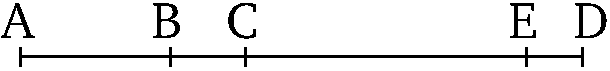
\includegraphics{Book09/fig23e.pdf}}

For let any  multitude whatsoever of odd numbers, $AB$, $BC$, $CD$,  lie together, and let the multitude of them be odd. I say that the whole, $AD$, is also odd.
 
For let the unit $DE$ be subtracted from $CD$. The remainder, $CE$,
is thus even [Def.~7.7]. And $CA$ is also even
[Prop.~9.22]. Thus, the whole, $AE$, is also even
[Prop.~9.21]. And $DE$ is a unit. Thus,
$AD$ is odd [Def.~7.7]. (Which is) the very thing it
was required to show.}
\end{Parallel}

%%%%%%
% Prop 9.24
%%%%%%
\pdfbookmark[1]{Proposition 9.24}{pdf9.24}
\begin{Parallel}{}{} 
\ParallelLText{
\begin{center}
{\large \ggn{24}.}
\end{center}\vspace*{-7pt}

\gr{Ἐὰν ἀπὸ ἀρτίου ἀριθμοῦ >άρτιοξ ἀφαιρεθῆ|, ὁ λοιπὸξ
>άρτιοξ >έσται.}

% Removed epsf size command
\centerline{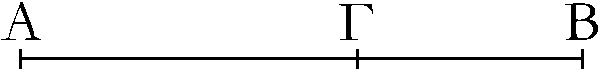
\includegraphics{Book09/fig24g.pdf}}

\gr{Ἀπὸ γὰρ ἀρτίου τοῦ ΑΒ >άρτιοξ ἀφῃρήσθω ὁ ΒΓ; λέγω, <ότι
ὁ λοιπὸξ ὁ ΓΑ >άρτιόξ ἐστιν.}

\gr{Ἐπεὶ γὰρ ὁ ΑΒ >άρτιόξ ἐστιν, >έθει μέροξ <ήμισυ.
διὰ τὰ α\kern -.7pt  ὐτὰ δὴ καὶ ὁ ΒΓ >έθει μέροξ <ήμισυ; <ώστε
καὶ λοιπὸξ [ὁ ΓΑ >έθει μέροξ <ήμισυ] >άρτιοξ [>άρα]
ἐστὶν ὁ ΑΓ; <όπερ >έδει δεῖχαι.}}

\ParallelRText{
\begin{center}
{\large Proposition 24}
\end{center}

If  an even (number) is subtracted from an(other) even
number then the remainder will be even.

% Removed epsf size command
\centerline{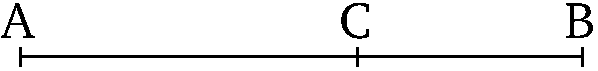
\includegraphics{Book09/fig24e.pdf}}

For let the even (number) $BC$ be subtracted from the even number
$AB$. I say that the remainder, $CA$, is even.

For since $AB$ is even, it has a half part [Def.~7.6]. 
So, for the same (reasons), $BC$ also has a half part. And hence the remainder [$CA$ has a half part]. [Thus,] $AC$ is even. (Which is) the very thing it was required to show.}
\end{Parallel}

%%%%%%
% Prop 9.25
%%%%%%
\pdfbookmark[1]{Proposition 9.25}{pdf9.25}
\begin{Parallel}{}{} 
\ParallelLText{
\begin{center}
{\large \ggn{25}.}
\end{center}\vspace*{-7pt}

\gr{Ἐὰν ἀπὸ ἀρτίου ἀριθμοῦ περισσὸξ ἀφαιρεθῆ|, ὁ λοιπὸξ
περισσὸξ >έσται.}

% Removed epsf size command
\centerline{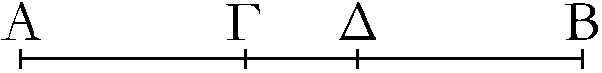
\includegraphics{Book09/fig25g.pdf}}

\gr{Ἀπὸ γὰρ ἀρτίου τοῦ ΑΒ περισσὸξ ἀφῃρήσθω ὁ ΒΓ; λέγω, <ότι
ὁ λοιπὸξ ὁ ΓΑ περισσόξ ἐστιν.}

\gr{Ἀφῃρήσθω γὰρ ἀπὸ τοῦ ΒΓ μονὰξ ἡ ΓΔ; ὁ ΔΒ >άρα >άρτιόξ
ἐστιν. >έστι δὲ καὶ ὁ ΑΒ >άρτιοξ; καὶ λοιπὸξ >άρα ὁ ΑΔ >άρτιόξ
ἐστιν. καί ἐστι μονὰξ ἡ ΓΔ; ὁ ΓΑ >άρα περισσόξ ἐστιν; <όπερ
>έδει δεῖχαι.}}

\ParallelRText{
\begin{center}
{\large Proposition 25}
\end{center}

If an odd (number) is subtracted from an even
number then the remainder will be odd.

% Removed epsf size command
\centerline{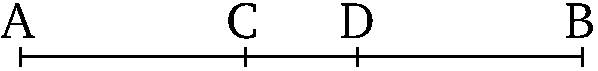
\includegraphics{Book09/fig25e.pdf}}

For let the odd (number) $BC$ be subtracted from the even number
$AB$. I say that the remainder $CA$ is odd.

For let the unit $CD$ be subtracted from $BC$. $DB$ is thus even
[Def.~7.7]. And $AB$ is also even. And thus the remainder $AD$ is even [Prop.~9.24]. And $CD$ is a unit. 
Thus, $CA$ is odd [Def.~7.7]. (Which is) the very thing it was required to show.}
\end{Parallel}

%%%%%%
% Prop 9.26
%%%%%%
\pdfbookmark[1]{Proposition 9.26}{pdf9.26}
\begin{Parallel}{}{} 
\ParallelLText{
\begin{center}
{\large \ggn{26}.}
\end{center}\vspace*{-7pt}

\gr{Ἐὰν ἀπὸ  περισσοῦ ἀριθμοῦ περισσὸξ ἀφαιρεθῆ|, ὁ λοιπὸξ >άρτιοξ
>έσται.}

% Removed epsf size command
\centerline{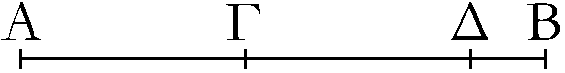
\includegraphics{Book09/fig26g.pdf}}

\gr{Ἀπὸ γὰρ περισσοῦ τοῦ ΑΒ περισσὸξ ἀφῃρήσθω ὁ ΒΓ; λέγω, <ότι
ὁ λοιπὸξ ὁ ΓΑ >άρτιόξ ἐστιν.}

\gr{Ἐπεὶ γὰρ ὁ ΑΒ περισσόξ ἐστιν, ἀφῃρήσθω μονὰξ ἡ ΒΔ; λοιπὸξ
>άρα ὁ ΑΔ >άρτιόξ ἐστιν. διὰ τὰ α\kern -.7pt  ὐτὰ δὴ καὶ ὁ ΓΔ >άρτιόξ
ἐστιν; <ώστε καὶ λοιπὸξ ὁ ΓΑ >άρτιόξ ἐστιν; <όπερ >έδει
δεῖχαι.}}

\ParallelRText{
\begin{center}
{\large Proposition 26}
\end{center}

If an odd (number) is subtracted from an odd
number then the remainder will be even.

% Removed epsf size command
\centerline{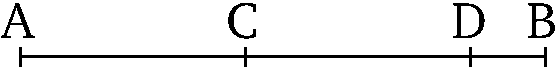
\includegraphics{Book09/fig26e.pdf}}

For let the odd (number) $BC$ be subtracted from the odd
(number) $AB$. I say that the remainder, $CA$, is even.

For since $AB$ is odd, let the unit $BD$ be subtracted (from it). 
Thus, the remainder $AD$ is even [Def.~7.7]. So, for the same (reasons), 
$CD$ is also even. And hence the remainder $CA$ is even [Prop.~9.24]. (Which is) the very thing it was required to show.}
\end{Parallel}

%%%%%%
% Prop 9.27
%%%%%%
\pdfbookmark[1]{Proposition 9.27}{pdf9.27}
\begin{Parallel}{}{} 
\ParallelLText{
\begin{center}
{\large \ggn{27}.}
\end{center}\vspace*{-7pt}

\gr{Ἐὰν ἀπὸ περισσοῦ ἀριθμοῦ >άρτιοξ ἀφαιρεθῆ|, ὁ λοιπὸξ περισσὸξ 
>έσται.}

% Removed epsf size command
\centerline{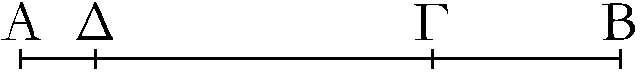
\includegraphics{Book09/fig27g.pdf}}

\gr{Ἀπὸ γὰρ περισσοῦ τοῦ ΑΒ >άρτιοξ ἀφῃρήσθω ὁ ΒΓ; λέγω, <ότι
ὁ λοιπὸξ ὁ ΓΑ περισσόξ ἐστιν.}

\gr{Ἀφῃρήσθω [γὰρ] μονὰξ ἡ ΑΔ; ὁ ΔΒ >άρα >άρτιόξ ἐστιν. >έστι
δὲ καὶ ὁ ΒΓ >άρτιοξ; καὶ λοιπὸξ >άρα ὁ ΓΔ >άρτιόξ ἐστιν.
περισσὸξ >άρα ὁ ΓΑ; <όπερ >έδει δεῖχαι.}}

\ParallelRText{
\begin{center}
{\large Proposition 27}
\end{center}

If an even (number) is subtracted from an odd
number then the remainder will be odd.

% Removed epsf size command
\centerline{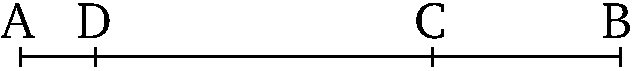
\includegraphics{Book09/fig27e.pdf}}

For let the even (number) $BC$ be subtracted from the odd (number)
$AB$. I say that the remainder, $CA$, is odd.

$[$For$]$ let the unit $AD$ be subtracted (from $AB$). $DB$ is thus
even [Def.~7.7]. And $BC$ is also even. Thus, the
remainder $CD$ is also even [Prop.~9.24]. 
$CA$ (is) thus odd [Def.~7.7]. (Which is) the
very thing it was required to show.}
\end{Parallel}

%%%%%%
% Prop 9.28
%%%%%%
\pdfbookmark[1]{Proposition 9.28}{pdf9.28}
\begin{Parallel}{}{} 
\ParallelLText{
\begin{center}
{\large \ggn{28}.}
\end{center}\vspace*{-7pt}

\gr{Ἐὰν περισσὸξ ἀριθμὸξ >άρτιον πολλαπλασιάσαξ ποιῆ| τινα, ὁ γενόμενοξ
>άρτιοξ >έσται.}

% Removed epsf size command
\centerline{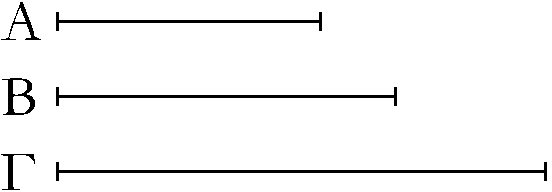
\includegraphics{Book09/fig28g.pdf}}

\gr{Περισσὸξ γὰρ ἀριθμὸξ ὁ Α >άρτιον τὸν Β πολλαπλασιάσαξ τὸν Γ ποιείτω;
λέγω, <ότι ὁ Γ >άρτιόξ ἐστιν.}

\gr{Ἐπεὶ γὰρ ὁ Α τὸν Β πολλαπλασιάσαξ τὸν Γ πεποίηκεν, ὁ Γ >άρα σύγκειται ἐκ τοσούτων >ίσων τῶ| Β, 
<όσαι εἰσὶν ἐν τῶ| Α μονάδεξ. καί ἐστιν ὁ Β >άρτιοξ;
ὁ Γ >άρα σύγκειται ἐχ ἀρτίων. ἒαν δὲ >άρτιοι ἀριθμοὶ
ὁποσοιοῦν συντεθῶσιν, ὁ <όλοξ >άρτιόξ ἐστιν. >άρτιοξ
>άρα ἐστὶν ὁ Γ; <όπερ >έδει δεῖχαι.}}

\ParallelRText{
\begin{center}
{\large Proposition 28}
\end{center}

If an odd number makes some (number by)
multiplying an even (number) then the created (number) will be even.

% Removed epsf size command
\centerline{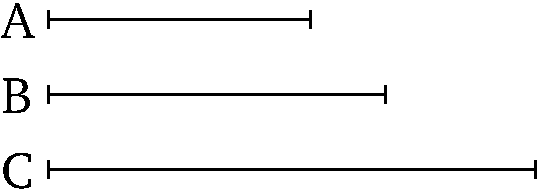
\includegraphics{Book09/fig28e.pdf}}

For let the odd number $A$ make $C$ (by) multiplying the even (number)
$B$. I say that $C$ is even.

For since $A$ has made $C$ (by) multiplying $B$, $C$ is thus composed  out of so many (magnitudes) equal to $B$, as many as (there) are  units in $A$ [Def.~7.15]. And $B$ is even. Thus, $C$ is composed
out of even (numbers). And if any multitude whatsoever of even numbers
is added together then the whole is even [Prop.~9.21]. 
Thus, $C$ is even. (Which is) the very thing it was required to show.}
\end{Parallel}

%%%%%%
% Prop 9.29
%%%%%%
\pdfbookmark[1]{Proposition 9.29}{pdf9.29}
\begin{Parallel}{}{} 
\ParallelLText{
\begin{center}
{\large \ggn{29}.}
\end{center}\vspace*{-7pt}

\gr{Ἐὰν περισσὸξ ἀριθμὸξ περισσὸν ἀριθμὸν πολλαπλασιάσ\-αξ ποιῆ|
τινα, ὁ γενόμενοξ περισσὸξ >έσται.}

% Removed epsf size command
\centerline{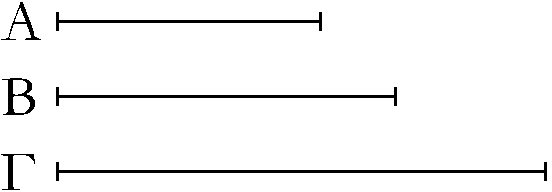
\includegraphics{Book09/fig28g.pdf}}

\gr{Περισσὸξ  γὰρ ἀριθμὸξ ὁ Α περισσὸν τὸν Β πολλαπλασιάσαξ τὸν Γ
ποιείτω; λέγω, <ότι ὁ Γ περισσόξ
ἐστιν.}

\gr{Ἐπεὶ γὰρ ὁ Α τὸν Β πολλαπλασιάσαξ τὸν Γ πεποίηκεν, ὁ Γ
>άρα σύγκειται ἐκ τοσούτων >ίσων τῶ| Β, <όσαι εἰσὶν ἐν τῶ|
Α μονάδεξ. καί ἐστιν ἑκάτεροξ τῶν Α, Β περισσόξ; ὁ Γ >άρα σύγκειται
ἐκ  περισσῶν ἀριθμῶν, <ῶν τὸ πλῆθοξ περισσόν ἐστιν. <ώστε
ὁ Γ περισσόξ ἐστιν; <όπερ >έδει δεῖχαι.}}

\ParallelRText{
\begin{center}
{\large Proposition 29}
\end{center}

If  an odd number makes some (number by)
multiplying an odd (number) then the created (number) will be odd.

% Removed epsf size command
\centerline{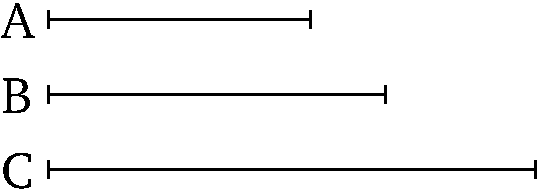
\includegraphics{Book09/fig28e.pdf}}

For let the odd number $A$ make $C$ (by) multiplying the odd (number)
$B$. I say that $C$ is odd.

For since $A$ has made $C$ (by) multiplying $B$, $C$ is thus composed  out of so many (magnitudes) equal to $B$, as many as (there) are  units in $A$ [Def.~7.15]. And each of $A$, $B$ is odd. Thus, $C$ is composed
out of odd (numbers), (and) the multitude of them is odd.   
Hence $C$ is odd [Prop.~9.23]. (Which is) the very thing it was required to show.}
\end{Parallel}

%%%%%%
% Prop 9.30
%%%%%%
\pdfbookmark[1]{Proposition 9.30}{pdf9.30}
\begin{Parallel}{}{} 
\ParallelLText{
\begin{center}
{\large \ggn{30}.}
\end{center}\vspace*{-7pt}

\gr{Ἐὰν περισσὸξ ἀριθμὸξ >άρτιον ἀριθμὸν μετρῆ|, καὶ τὸν <ήμισυν
α\kern -.7pt  ὐτοῦ μετρήσει.}

% Removed epsf size command
\centerline{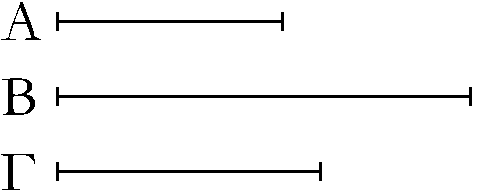
\includegraphics{Book09/fig30g.pdf}}

\gr{Περισσὸξ γὰρ ἀριθμὸξ ὁ Α >άρτιον τὸν Β μετρείτω; λέγω, <ότι
καὶ τὸν <ήμισυν α\kern -.7pt  ὐτοῦ μετρήσει.}

\gr{Ἐπεὶ γὰρ ὁ Α τὸν Β μετρεῖ, μετρείτω α\kern -.7pt  ὐτὸν κατὰ τὸν  Γ; λέγω,
<ότι ὁ Γ οὐκ >έστι περισσόξ. εἰ γὰρ δυνατόν, >έστω. καὶ ἐπεὶ
ὁ Α τὸν Β μετρεῖ κατὰ τὸν Γ, ὁ Α >άρα τὸν Γ πολλαπλασιάσαξ
τὸν Β πεποίηκεν. ὁ Β >άρα σύγκειται ἐκ περισσῶν ἀριθμῶν,
<ῶν τὸ πλῆθοξ περισσόν ἐστιν. ὁ Β >άρα περισσόξ ἐστιν; <όπερ
>άτοπον; ὑπόκειται γὰρ >άρτιοξ. οὐκ >άρα ὁ Γ περισσόξ ἐστιν;
>άρτιοξ >άρα ἐστὶν ὁ Γ. <ώστε ὁ Α τὸν Β μετρεῖ ἀρτιάκιξ.
διὰ δὴ τοῦτο καὶ τὸν <ήμισυν α\kern -.7pt  ὐτοῦ μετρήσει; <όπερ >έδει
δεῖχαι.}}

\ParallelRText{
\begin{center}
{\large Proposition 30}
\end{center}

If an odd number measures an even number then it
will also measure (one) half of it.

% Removed epsf size command
\centerline{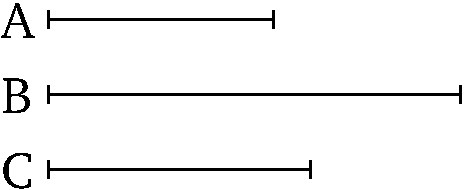
\includegraphics{Book09/fig30e.pdf}}

For let the odd number $A$ measure the even (number) $B$. I say that
($A$) will also measure (one) half of ($B$).

For since $A$ measures $B$, let it measure it according to $C$. I say that
$C$ is not odd. For, if possible, let it be (odd). And since $A$ measures $B$ according to $C$, $A$ has thus made $B$ (by) multiplying $C$. Thus, $B$
is composed out of odd numbers, (and) the multitude of them is odd. $B$
is thus odd [Prop.~9.23]. The very thing (is)
absurd. For ($B$) was assumed (to be) even. Thus, $C$ is not odd.
Thus, $C$ is even. Hence, $A$ measures $B$ an even number of times.
So, on account of this, ($A$) will also measure (one) half of ($B$).
(Which is) the very thing it was required to show.}
\end{Parallel}

%%%%%%
% Prop 9.31
%%%%%%
\pdfbookmark[1]{Proposition 9.31}{pdf9.31}
\begin{Parallel}{}{} 
\ParallelLText{
\begin{center}
{\large \ggn{31}.}
\end{center}\vspace*{-7pt}

\gr{Ἐὰν περισσὸξ ἀριθμὸξ πρόξ τινα ἀριθμὸν πρῶτοξ >ῆ|, καὶ πρὸξ
τὸν διπλασίονα α\kern -.7pt  ὐτοῦ πρῶτοξ >έσται.}

% Removed epsf size command
\centerline{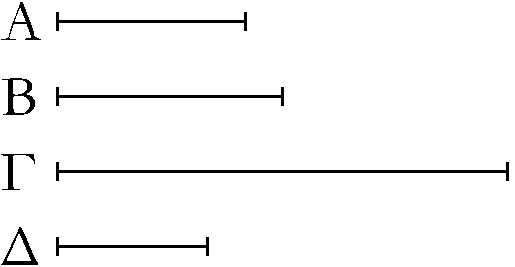
\includegraphics{Book09/fig31g.pdf}}

\gr{Περισσὸξ γὰρ ἀριθμὸξ ὁ Α πρόξ τινα ἀριθμὸν τὸν Β πρῶτοξ >έστω,
τοῦ δὲ Β διπλασίων >έστω ὁ Γ; λέγω, <ότι ὁ Α [καὶ]
πρὸξ τὸν Γ πρῶτόξ ἐστιν.}

\gr{Εἰ γὰρ μ\kern -.7pt  ή εἰσιν [οἱ Α, Γ] πρῶτοι, μετρήσει τιξ α\kern -.7pt  ὐτοὺξ ἀριθμόξ.
μετρείτω, καὶ >έστω ὁ Δ. καί ἐστιν ὁ Α περισσόξ; περισσὸξ >άρα καὶ
ὁ Δ. καὶ ἐπεὶ ὁ Δ περισσὸξ >ὼν τὸν Γ μετρεῖ, καί ἐστιν ὁ Γ
>άρτιοξ, καὶ τὸν <ήμισυν >άρα τοῦ  Γ μετρήσει [ὁ Δ]. τοῦ δὲ
Γ <ήμισύ ἐστιν ὁ Β; ὁ Δ >άρα τὸν Β μετρεῖ. μετρεῖ δὲ καὶ τὸν Α.
ὁ Δ >άρα τοὺξ Α, Β μετρεῖ πρώτουξ >όνταξ πρὸξ ἀλλήλουξ;
<όπερ ἐστὶν ἀδύνατον. οὐκ >άρα ὁ Α πρὸξ τὸν Γ πρῶτοξ ο>ύκ
ἐστιν. οἱ Α, Γ >άρα πρῶτοι πρὸξ ἀλλήλουξ εἰσίν; <όπερ >έδει
δεῖχαι.}}

\ParallelRText{
\begin{center}
{\large Proposition 31}
\end{center}

If an odd number is prime to some number then it
will also be prime to its double.

% Removed epsf size command
\centerline{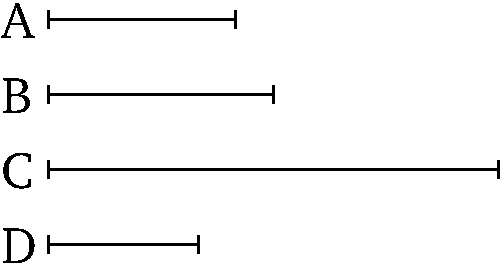
\includegraphics{Book09/fig31e.pdf}}

For let the odd number $A$ be prime to some number $B$. And let $C$ be
double $B$. I say that $A$ is [also] prime to $C$.

For if [$A$ and $C$] are not prime (to one another) then some number
will measure them. Let it measure (them), and let it be $D$. And
$A$ is odd. Thus, $D$ (is) also odd. And since $D$, which is odd, measures
$C$, and $C$ is even, [$D$] will thus also measure half of $C$ [Prop.~9.30]. 
And $B$ is half of $C$.  Thus, $D$ measures $B$. And it also measures
$A$. Thus, $D$ measures (both) $A$ and $B$, (despite) them being prime to one another. The very thing is impossible. Thus, $A$ is not unprime 
to $C$. Thus, $A$ and $C$ are prime to one another. (Which is) the very thing it
was required to show.}
\end{Parallel}

%%%%%%
% Prop 9.32
%%%%%%
\pdfbookmark[1]{Proposition 9.32}{pdf9.32}
\begin{Parallel}{}{} 
\ParallelLText{
\begin{center}
{\large\ggn{32}.}
\end{center}\vspace*{-7pt}

\gr{Τῶν ἀπὸ δύαδοξ διπλασιαζομένων ἀριθμων <έκαστοξ ἀρτιάκιξ
>άρτιόξ ἐστι μόνον.}

% Removed epsf size command
\centerline{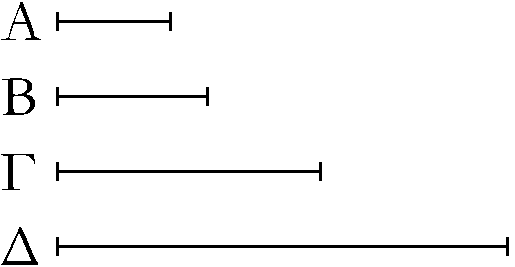
\includegraphics{Book09/fig32g.pdf}}

\gr{Ἀπὸ γὰρ δύαδοξ τῆξ Α δεδιπλασιάσθωσαν ὁσοιδηποτοῦν ἀριθμοὶ
οἱ Β, Γ, Δ; λέγω, <ότι οἱ Β, Γ, Δ ἀρτιάκιξ >άρτιοί εἰσι μόνον.}

\gr{<'Οτι μὲν ο>ῦν <έκαστοξ [τῶν Β, Γ, Δ] ἀρτιάκιξ >άρτιόξ
ἐστιν, φανερόν; ἀπὸ γὰρ δυάδοξ ἐστὶ διπλασιασθείξ. λέγω, <ότι
καὶ μόνον. ἐκκείσθω γὰρ μονάξ. ἐπεὶ ο>ῦν ἀπὸ μονάδοξ
ὁποσοιοῦν ἀριθμοὶ ἑχῆξ ἀνάλογόν εἰσιν, ὁ δὲ μετὰ τὴν
μονάδα ὁ Α πρῶτόξ ἐστιν, ὁ μέγιστοξ τῶν Α, Β, Γ, Δ ὁ Δ ὑπ>
οὐδενὸξ >άλλου μετρηθήσεται παρὲχ τῶν Α, Β, Γ. καί ἐστιν <έκαστοξ
τῶν Α, Β, Γ >άρτιοξ; ὁ Δ >άρα ἀρτιάκιξ >άρτιόξ ἐστι μόνον.
ὁμοίωξ δὴ δείχομεν, <ότι [καὶ] ἑκάτεροξ τῶν Β, Γ
ἀρτιάκιξ >άρτιόξ ἐστι μόνον; <όπερ >έδει δεῖχαι.}}

\ParallelRText{
\begin{center}
{\large Proposition 32}
\end{center}

Each of the numbers (which is continually) doubled,
(starting) from a dyad, is an even-times-even (number) only.

% Removed epsf size command
\centerline{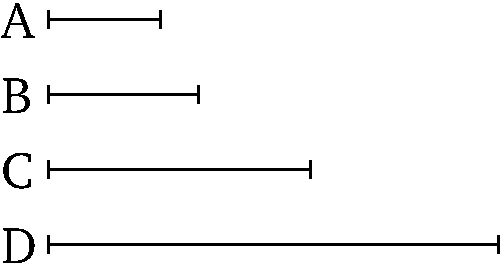
\includegraphics{Book09/fig32e.pdf}}

For let any multitude of numbers whatsoever, $B$, $C$, $D$, be
(continually) doubled, (starting) from the dyad $A$. I say that
$B$, $C$, $D$ are  even-times-even (numbers) only.

In fact, (it is) clear that each [of $B$, $C$, $D$] is an even-times-even (number). For it is doubled from a dyad [Def.~7.8]. 
I also say that (they are even-times-even numbers) only. For let a unit
be laid down. Therefore, since any multitude of numbers whatsoever
are continuously proportional, starting from a unit, and the (number) $A$ after the unit is prime, the greatest of $A$, $B$, $C$, $D$, (namely) $D$,
will not be measured by any other (numbers) except $A$, $B$, $C$
[Prop.~9.13].
And each of $A$, $B$, $C$ is even. Thus, $D$ is an
even-time-even (number) only [Def.~7.8]. So, similarly,
we can show that each of $B$, $C$ is [also]  an even-time-even (number) only. (Which is) the very thing it was required to show.}
\end{Parallel}

%%%%%%
% Prop 9.33
%%%%%%
\pdfbookmark[1]{Proposition 9.33}{pdf9.33}
\begin{Parallel}{}{} 
\ParallelLText{
\begin{center}
{\large \ggn{33}.}
\end{center}\vspace*{-7pt}

\gr{Ἐὰν ἀριθμὸξ τὸν <ήμισυν >έθῃ περισσόν, ἀρτιάκιξ περισσόξ ἐστι
μόνον.}

% Removed epsf size command
\centerline{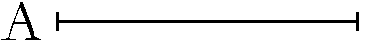
\includegraphics{Book09/fig33g.pdf}}

\gr{Ἀριθμὸξ γὰρ ὁ Α τὸν <ήμισυν ἐθέτω περισσόν; λέγω, <ότι ὁ Α
ἀρτιάκιξ περισσόξ ἐστι μόνον.}

\gr{<'Οτι μὲν ο>ῦν ἀρτιάκιξ περισσόξ ἐστιν, φανερόν; ὁ γὰρ <ήμισυξ
α\kern -.7pt  ὐτοῦ περισσὸξ >ὼν μετρεῖ α\kern -.7pt  ὐτὸν ἀρτιάκιξ, λέγω δή, <ότι
καὶ μόνον. εἰ γὰρ >έσται ὁ Α καὶ ἀρτιάκιξ >άρτιοξ, μετρηθήσεται
ὑπὸ ἀρτίου κατὰ >άρτιον ἀριθμόν; <ώστε καὶ ὁ <ήμισυξ α\kern -.5pt  ὐτοῦ
μετρηθήσεται ὑπὸ ἀρτίου ἀριθμοῦ περισσὸξ >ών; <όπερ ἐστὶν
>άτοπον. ὁ Α >άρα ἀρτιάκιξ περισσόξ ἐστι μόνον; <όπερ
>έδει δεῖχαι.}}

\ParallelRText{
\begin{center}
{\large Proposition 33}
\end{center}

If a number has an odd half then it is an
even-time-odd (number) only.

% Removed epsf size command
\centerline{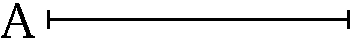
\includegraphics{Book09/fig33e.pdf}}

For let the number $A$ have an odd half. I say that $A$ is  an
even-times-odd (number) only.

In fact, (it is) clear that ($A$) is an even-times-odd (number). For its
half, being odd, measures it an even number of times [Def.~7.9]. So I also say that (it is an even-times-odd number) only. For if $A$ is also  an even-times-even
(number) then it will be measured by an even (number) according to
an even number [Def.~7.8]. Hence, its half
will also be measured by an even number, (despite)  being odd. The very
thing is absurd. Thus, $A$ is  an even-times-odd (number) only. (Which is)
the very thing it was required to show.}
\end{Parallel}

%%%%%%
% Prop 9.34
%%%%%%
\pdfbookmark[1]{Proposition 9.34}{pdf9.34}
\begin{Parallel}{}{} 
\ParallelLText{
\begin{center}
{\large \ggn{34}.}
\end{center}\vspace*{-7pt}

\gr{Ἐὰν ἀριθμὸξ μ\kern -.7pt  ήτε τῶν ἀπὸ δυάδοξ διπλασιαζομένων >ῆ|, μ\kern -.7pt  ήτε
τὸν <ήμισυν >έθῃ περισσόν, ἀρτιάκιξ τε >άρτιόξ ἐστι καὶ ἀρτιάκιξ
περισσόξ.}

% Removed epsf size command
\centerline{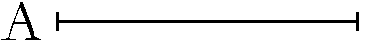
\includegraphics{Book09/fig33g.pdf}}

\gr{Ἀριθμὸξ γὰρ ὁ Α μ\kern -.7pt  ήτε τῶν ἀπὸ δυάδοξ διπλασιαζομένων >έστω
μ\kern -.7pt  ήτε τὸν <ήμισυν ἐθέτω περισσόν; λέγω, <ότι ὁ Α ἀρτιάκιξ
τέ ἐστιν >άρτιοξ καὶ ἀρτιάκιξ περισσόξ.}

\gr{<'Οτι μὲν ο>ῦν ὁ Α ἀρτιάκιξ ἐστὶν >άρτιοξ, φανερόν; τὸν γὰρ
<ήμισυν οὐκ >έθει περισσόν. λέγω δή, <ότι καὶ ἀρτιάκιξ περισσόξ
ἐστιν. ἒαν γὰρ τὸν Α τέμνωμεν δίθα καὶ τὸν <ήμισυν α\kern -.7pt  ὐτοῦ
δίθα καὶ τοῦτο ἀεὶ ποιῶμεν, καταντήσομεν ε>ίξ τινα
ἀριθμὸν περισσόν, <ὸξ μετρήσει τὸν Α κατὰ >άρτιον ἀριθμόν. εἰ γὰρ
ο>ύ, καταντήσομεν εἰξ
δυάδα, καὶ
>έσται ὁ Α τῶν ἀπὸ δυάδοξ διπλασιαζομένων; <όπερ οὐθ
ὑπόκειται. <ώστε ὁ Α ἀρτιάκιξ περισσόν ἐστιν. ἐδείθθη δὲ καὶ
ἀρτιάκιξ >άρτιοξ. ὁ Α >άρα ἀρτιάκιξ τε >άρτιόξ ἐστι καὶ ἀρτιάκιξ
περισσόξ; <όπερ >έδει δεῖχαι.}}

\ParallelRText{
\begin{center}
{\large Proposition 34}
\end{center}

If a number is neither (one) of the (numbers) doubled from a dyad, nor
has an odd half, then it is (both) an even-times-even and an even-times-odd
(number).

% Removed epsf size command
\centerline{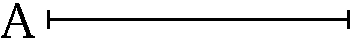
\includegraphics{Book09/fig33e.pdf}}

For let the number $A$   neither be (one) of the (numbers) doubled from a
dyad, nor let it have an odd half. I say that $A$ is (both) an even-times-even
and an even-times-odd (number).

In fact, (it is) clear that $A$ is an even-times-even (number) [Def.~7.8]. For it does
not have an odd half. So I say that it is also an even-times-odd (number). 
For if we cut $A$ in half, and (then cut) its half in half, and we do this continually, then we will arrive at some odd number which will measure
$A$ according to an even number. For if not, we will arrive at a dyad,
and $A$ will be (one) of the (numbers) doubled from a dyad. The very opposite thing (was) assumed. Hence, $A$ is an even-times-odd (number)
[Def.~7.9]. And it was also shown (to be) an
even-times-even (number). Thus, $A$ is (both) an even-times-even and
an even-times-odd (number). (Which is) the very thing it was required to
show.}
\end{Parallel}

%%%%%%
% Prop 9.35
%%%%%%
\pdfbookmark[1]{Proposition 9.35}{pdf9.35}
\begin{Parallel}{}{} 
\ParallelLText{
\begin{center}
{\large \ggn{35}.}
\end{center}\vspace*{-7pt}

\gr{Ἐὰν >ῶσιν ὁσοιδηποτοῦν ἀριθμοὶ ἑχῆξ ἀνάλογον, ἀφαιρεθῶσι δὲ ἀπό τε τοῦ δευτέρου καὶ τοῦ ἐσθάτου >ίσοι τῶ| πρώτῳ, >έσται
ὡξ ἡ τοῦ δευτέρου ὑπεροθὴ πρὸξ τὸν πρῶτον, ο<ύτωξ ἡ τοῦ
ἐσθάτου ὑπεροθὴ πρὸξ τοὺξ πρὸ ἑαυτοῦ πάνταξ.}\\

% Removed epsf size command
\centerline{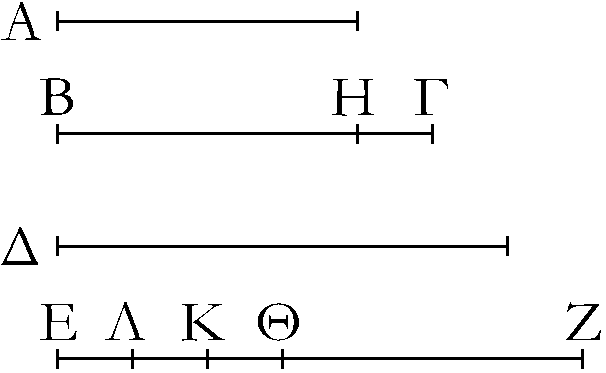
\includegraphics{Book09/fig35g.pdf}}

\gr{>'Εστωσαν ὁποσοιδηποτοῦν ἀριθμοὶ ἑχῆξ ἀνάλογον
οἱ Α, ΒΓ, Δ, ΕΖ ἀφθόμενοι ἀπὸ ἐλαθίστου τοῦ Α, καὶ ἀφῃρήσθω ἀπὸ τοῦ ΒΓ καὶ τοῦ ΕΖ τὼ| Α >ίσοξ ἑκάτεροξ τῶν ΒΗ, ΖΘ; λέγω, <ότι ἐστὶν ὡξ ὁ ΗΓ πρὸξ τὸν Α, ο<ύτωξ ὁ ΕΘ πρὸξ τοὺξ Α, ΒΓ, Δ.}

\gr{Κείσθω γὰρ τῶ| μὲν ΒΓ >ίσοξ ὁ ΖΚ, τῶ| δὲ Δ >ίσοξ ὁ  ΖΛ. καὶ
ἐπεὶ ὁ ΖΚ τῶ| ΒΓ >ίσοξ
 ἐστίν, <ῶν ὁ ΖΘ τῶ| ΒΗ >ίσοξ ἐστίν, λοιπὸξ >άρα ὁ ΘΚ λοιπῶ|
 τῶ| ΗΓ ἐστιν >ίσοξ.
καὶ ἐπεί ἐστιν ὡξ ὁ ΕΖ πρὸξ τὸν Δ, ο<ύτωξ ὁ Δ πρὸξ τὸν ΒΓ καὶ
ὁ ΒΓ πρὸξ τὸν Α, >ίσοξ δὲ ὁ μὲν Δ τῶ| ΖΛ, ὁ δὲ ΒΓ τῶ| ΖΚ, ὁ
δὲ Α τῶ| ΖΘ, >έστιν >άρα ὡξ ὁ ΕΖ πρὸξ τὸν ΖΛ, ο<ύτωξ ὁ ΛΖ πρὸξ
τὸν ΖΚ καὶ ὁ ΖΚ πρὸξ τὸν ΖΘ. διελόντι, ὡξ ὁ ΕΛ πρὸξ τὸν ΛΖ, ο<ύτωξ ὁ ΛΚ πρὸξ τὸν ΖΚ καὶ ὁ ΚΘ πρὸξ τὸν ΖΘ. >έστιν >άρα καὶ
ὡξ ε<ῖξ τῶν ἡγουμένων πρὸξ <ένα τῶν ἑπομένων, ο<ύτωξ
<άπαντεξ οἱ ἡγούμενοι πρὸξ <άπανταξ τοὺξ ἑπομένουξ; >έστιν
>άρα ὡξ ὁ ΚΘ πρὸξ τὸν ΖΘ, ο<ύτωξ οἱ ΕΛ, ΛΚ, ΚΘ πρὸξ τοὺξ ΛΖ, ΖΚ,
ΘΖ.  >ίσοξ δὲ ὁ μὲν ΚΘ τῶ| ΓΗ, ὁ δὲ ΖΘ τῶ| Α, οἱ δὲ ΛΖ, ΖΚ, ΘΖ
τοὶξ Δ, ΒΓ, Α; >έστιν >άρα ὡξ ὁ ΓΗ  πρὸξ τὸν  Α, ο<ύτωξ ὁ ΕΘ πρὸξ τοὺξ Δ, ΒΓ, Α. >έστιν >άρα ὡξ ἡ τοῦ δευτέρου ὑπεροθὴ πρὸξ
τὸν πρῶτον, ο<ύτωξ ἡ τοῦ
ἐσθάτου ὑπεροθὴ πρὸξ τοὺξ πρὸ ἑαυτοῦ πάνταξ;
<όπερ >έδει δεῖχαι.}}

\ParallelRText{
\begin{center}
{\large Proposition 35}$^\dag$
\end{center}

If there is any multitude whatsoever of continually
proportional numbers, and (numbers) equal to the first are subtracted from (both) the
second and the last, then as the excess of the second (number is) to the first, so
the excess of the last will be to (the sum of) all   those (numbers) before it.

% Removed epsf size command
\centerline{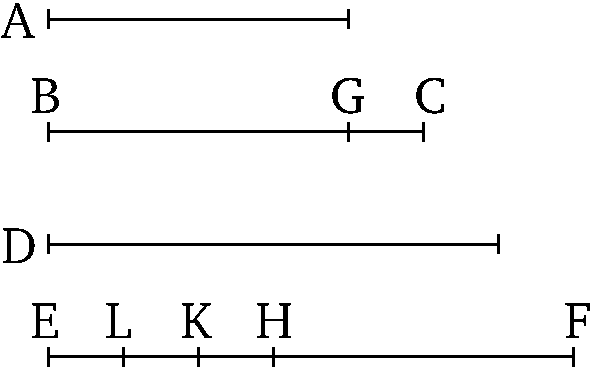
\includegraphics{Book09/fig35e.pdf}}

Let $A$, $BC$, $D$, $EF$ be any multitude whatsoever of continuously proportional numbers, beginning from the least $A$.  And let $BG$ and
$FH$, each equal to $A$, be subtracted from $BC$ and $EF$ (respectively). I say that as $GC$ is to $A$, so $EH$ is to $A$, $BC$, $D$.

For let $FK$ be made equal to $BC$, and $FL$ to  $D$. And since $FK$
is equal to $BC$, of which $FH$ is equal to $BG$, the remainder,
$HK$,  is thus equal to the remainder, $GC$. And since as $EF$ is to $D$, so
$D$ (is) to $BC$, and $BC$ to $A$ [Prop.~7.13],
and $D$ (is) equal to $FL$, and $BC$ to $FK$, and $A$ to  $FH$, thus
as $EF$ is to $FL$, so $LF$ (is) to $FK$, and $FK$ to $FH$. By
separation, as $EL$ (is) to $LF$, so $LK$ (is) to $FK$, and $KH$ to $FH$
[Props.~7.11, 7.13]. And thus
as one of the leading (numbers) is to one of the following, so (the sum of) all of the leading (numbers is) to (the sum of) all of the following [Prop.~7.12]. Thus, as $KH$ is to $FH$, so
$EL$, $LK$, $KH$ (are) to $LF$, $FK$, $HF$.  And $KH$ (is) equal to
$CG$, and $FH$ to $A$, and $LF$, $FK$, $HF$ to $D$, $BC$, $A$.
Thus, as $CG$ is to $A$, so $EH$ (is) to $D$, $BC$, $A$. Thus,
as the excess of the second (number) is to the first, so the excess of the last
(is) to (the sum of) all  those (numbers) before it. (Which is) the very thing it was required to show.}
\end{Parallel}
{\footnotesize\noindent$^\dag$ This proposition allows us to sum a geometric series of the form $a$, $a\,r$, $a\,r^2$, $a\,r^3,\cdots a\,r^{n-1}$. 
According to Euclid, the sum, $S_n$,  satisfies
$(a\,r-a)/a = (a\,r^n-a)/S_n$. Hence, $S_n= a\,(r^n-1)/(r-1)$.}

%%%%%%
% Prop 9.36
%%%%%%
\pdfbookmark[1]{Proposition 9.36}{pdf9.36}
\begin{Parallel}{}{} 
\ParallelLText{
\begin{center}
{\large \ggn{36}.}
\end{center}\vspace*{-7pt}

\gr{Ἐὰν ἀπὸ μονάδοξ ὁποσοιοῦν ἀριθμοὶ ἑχῆξ ἐκτεθῶσιν ἐν τῆ|
διπλασίονι ἀναλογίᾳ, <έωξ ο<ῦ ὁ σύμπαξ συντεθεὶξ πρῶτοξ
γένηται, καὶ ὁ σύμπαξ ἐπὶ τὸν >έσθατον πολλαπλασιασθεὶξ
ποιῆ| τινα, ὁ γενόμενοξ τέλειοξ >έσται.}

\gr{Ἀπὸ γὰρ μονάδοξ ἐκκείσθωσαν ὁσοιδηποτοῦν ἀριθμ\-οὶ
ἐν τῆ| διπλασίονι ἀναλογίᾳ, <έωξ ο<ῦ ὁ σύμπαξ συντεθεὶξ
πρῶτοξ γένηται, οἱ Α, Β, Γ, Δ, καὶ τῶ| σύμπαντι >ίσοξ
>έστω ὁ Ε, καὶ ὁ Ε τὸν Δ πολλαπλασιάσαξ τὸν ΖΗ ποιείτω. λέγω,
<ότι ὁ ΖΗ τέλειόξ ἐστιν.}\\

% Removed epsf size command
\centerline{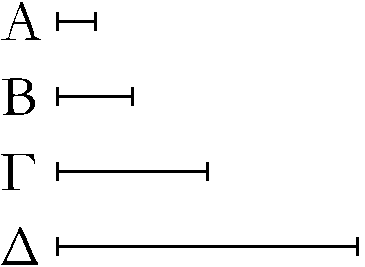
\includegraphics{Book09/fig36g.pdf}}}

\ParallelRText{
\begin{center}
{\large Proposition 36}$^\dag$
\end{center}

If any multitude whatsoever of numbers is set out
continuously 
in a double  proportion, (starting) from a  unit,
until the whole sum added together becomes  prime, and the sum multiplied
into the last (number) makes some (number), then the (number so) created
will be perfect.

For let any multitude of numbers, $A$, $B$, $C$, $D$, be set out (continuouly) in a
double proportion, until the whole sum added together is made  prime. And let $E$ be equal to the sum. And let $E$ make $FG$ (by) multiplying $D$. I say that $FG$ is a perfect (number).

% Removed epsf size command
\centerline{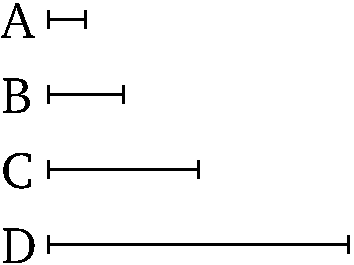
\includegraphics{Book09/fig36e.pdf}}
}
\end{Parallel}~\\

\begin{Parallel}{}{} 
\ParallelLText{
% Removed epsf size command
\centerline{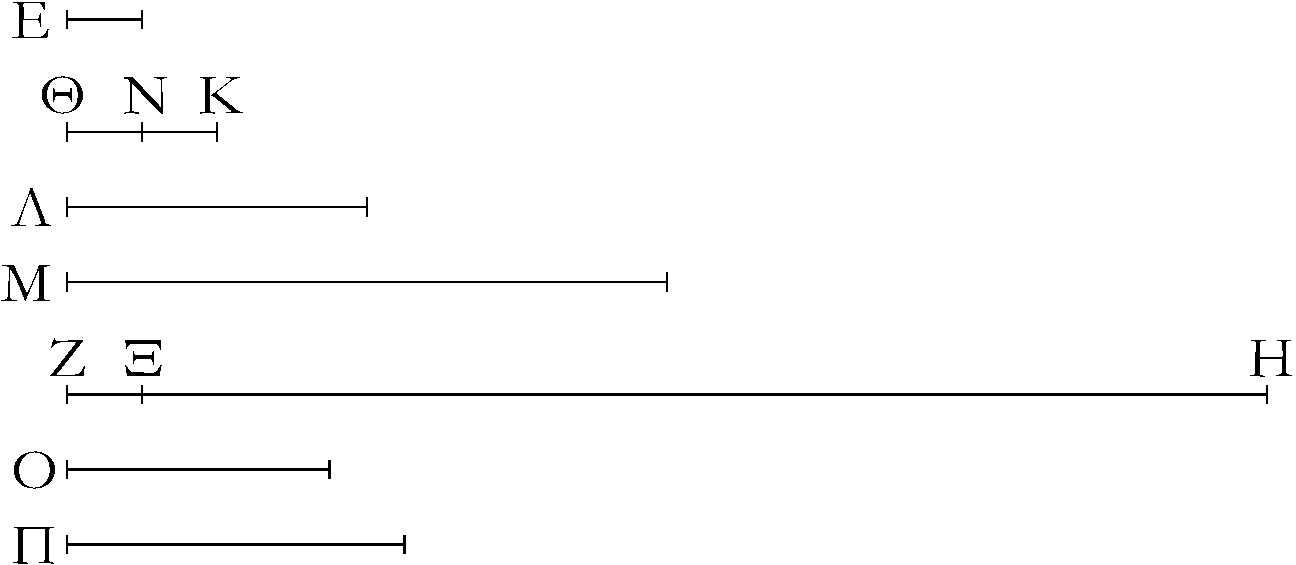
\includegraphics{Book09/fig36ag.pdf}}

\gr{<'Οσοι γάρ εἰσιν οἱ Α, Β, Γ, Δ τῶ| πλήθει, τοσοῦτοι
ἀπὸ τοῦ Ε εἰλήφθωσαν ἐν τῆ| διπλασίονι ἀναλογίᾳ οἱ 
Ε, ΘΚ, Λ, Μ; δι> >ίσου >άρα ἐστὶν ὡξ ὁ Α πρὸξ τὸν Δ, ο<ύτωξ
ὁ Ε πρὸξ τὸν Μ. ὁ >άρα ἐκ τῶν Ε, Δ >ίσοξ ἐστὶ τῶ| ἐκ τῶν
Α, Μ. καί ἐστιν ὁ ἐκ τῶν Ε, Δ 
ὁ ΖΗ; καὶ ὁ ἐκ τῶν
Α, Μ >άρα ἐστὶν ὁ ΖΗ. ὁ Α >άρα τὸν Μ πολλαπλασιάσαξ τὸν ΖΗ
πεποίηκεν; ὁ Μ >άρα τὸν ΖΗ μετρεῖ κατὰ τὰξ ἐν τῶ| Α μονάδαξ.
καί ἐστι δυὰξ ὁ Α; διπλάσιοξ  >άρα ἐστὶν ὁ ΖΗ τοῦ Μ.
εἰσὶ δὲ καὶ οἱ Μ, Λ, ΘΚ, Ε ἑχῆξ διπλάσιοι ἀλλήλων; οἱ
Ε, ΘΚ, Λ, Μ, ΖΗ >άρα ἑχῆξ ἀνάλογόν εἰσιν ἐν τῆ| διπλασίονι ἀναλογίᾳ. ἀφῃρήσθω δὴ ἀπὸ τοῦ δευτέρου τοῦ ΘΚ καὶ τοῦ
ἐσθάτου τοῦ ΖΗ τῶ| πρώτῳ τῶ| Ε >ίσοξ ἑκάτεροξ τῶν ΘΝ, ΖΧ;
>έστιν >άρα ὡξ ἡ τοῦ δευτέρου ἀριθμοῦ ὑπεροθὴ πρὸξ
τὸν πρῶτον, ο<ύτωξ ἡ τοῦ ἐσθάτου ὑπεροθὴ πρὸξ τοὺξ πρὸ
ἑαυτοῦ πάνταξ. >έστιν >άρα ὡξ ὁ ΝΚ πρὸξ τὸν Ε, ο<ύτωξ
ὁ ΧΗ πρὸξ τοὺξ Μ, Λ, ΚΘ, Ε. καί ἐστιν ὁ ΝΚ >ίσοξ τῶ| Ε;
καὶ ὁ ΧΗ >άρα >ίσοξ ἐστὶ τοῖξ Μ, Λ, ΘΚ, Ε. >έστι δὲ καὶ
ὁ ΖΧ τῶ| Ε >ίσοξ, ὁ δὲ Ε τοῖξ Α, Β, Γ, Δ καὶ τῆ| μονάδι. <όλοξ
>άρα ὁ ΖΗ >ίσοξ ἐστὶ τοῖξ τε Ε, ΘΚ, Λ, Μ καὶ τοῖξ Α, Β, Γ, Δ καὶ τῆ|
μονάδι; καὶ μετρεῖται ὑπ> α\kern -.7pt  ὐτῶν. λέγω, <ότι καὶ ὁ ΖΗ ὐπ> οὐδενὸξ >άλλου μετρηθήσεται παρὲχ τῶν Α, Β, Γ, Δ, Ε, ΘΚ, Λ, Μ καὶ
τῆξ μονάδοξ. εἰ γὰρ δυνατόν, μετρείτω τιξ τὸν ΖΗ ὁ Ο, καὶ ὁ Ο
μ\kern -.7pt  ηδενὶ τῶν Α, Β, Γ, Δ, Ε, ΘΚ, Λ, Μ >έστω ὁ α\kern -.5pt  ὐτόξ. καὶ ὁσάκιξ
ὁ Ο τὸν ΖΗ μετρεῖ, τοσα\kern -.3pt  ῦται μονάδεξ >έστωσαν ἐν τῶ| Π; ὁ Π
>άρα τὸν Ο πολλαπλασιάσαξ τὸν ΖΗ πεποίηκεν. ἀλλὰ μ\kern -.7pt  ὴν καὶ ὁ Ε
τὸν Δ πολλαπλασιάσαξ τὸν ΖΗ πεποίηκεν; >έστιν >άρα ὡξ ὁ Ε πρὸξ
τὸν Π, ὁ Ο πρὸξ τὸν Δ. καὶ ἐπεὶ ἀπὸ μονάδοξ ἑχῆξ
ἀνάλογόν εἰσιν οἱ Α, Β, Γ, Δ, ὁ Δ >άρα ὑπ> οὐδενὸξ >άλλου
ἀριθμοῦ μετρηθήσεται παρὲχ τῶν Α, Β, Γ. καὶ ὑπόκειται ὁ Ο οὐδενὶ
τῶν Α, Β, Γ ὁ α\kern -.7pt  ὐτόξ; οὐκ >άρα μετρήσει ὁ Ο τὸν Δ. ἀλλ> ὡξ ὁ Ο
πρὸξ τὸν Δ, ὁ Ε πρὸξ τὸν Π; οὐδὲ ὁ Ε >άρα τὸν Π μετρεῖ. καί
ἐστιν ὁ Ε πρῶτοξ; πᾶξ δὲ πρῶτοξ ἀριθμὸξ πρὸξ
<άπαντα, <ὸν μ\kern -.7pt  ὴ μετρεῖ, πρῶτόξ [ἐστιν]. οἱ Ε, Π
>άρα πρῶτοι πρὸξ ἀλλήλουξ εἰσίν. οἱ δὲ πρῶτοι καὶ
ἐλάθιστοι, οἱ δὲ ἐλάθιστοι μετροῦσι τοὺξ τὸν α\kern -.7pt  ὐτὸν λόγον >έθονταξ
ἰσάκιξ  <ό τε ἡγούμενοξ τὸν  ἡγούμενον καὶ ὁ  ἑπόμενοξ τὸν
ἑπόμενον; καί ἐστιν ὡξ ὁ Ε πρὸξ τὸν Π, ὁ Ο
πρὸξ τὸν Δ;  ἰσάκιξ >άρα ὁ Ε τὸν Ο μετρεῖ καὶ ὁ Π τὸν Δ.
 ὁ δὲ Δ ὑπ> οὐδενὸξ >άλλου μετρεῖται
παρὲχ τῶν Α, Β, Γ; ὁ Π >άρα ἑνὶ τῶν Α, Β, Γ ἐστιν ὁ α\kern -.7pt  ὐτόξ. >έστω
τῶ| Β ὁ α\kern -.7pt  ὐτόξ. καὶ <όσοι εἰσὶν οἱ Β, Γ, Δ τῶ| πλήθει τοσοῦτοι
εἰλήφθωσαν ἀπὸ τοῦ Ε οἱ Ε, ΘΚ, Λ. καί εἰσιν οἱ Ε, ΘΚ, Λ τοῖξ
Β, Γ, Δ ἐν τῶ| α\kern -.7pt  ὐτῶ| λόγω; δι> >ίσου >άρα ἐστὶν ὡξ ὁ Β πρὸξ
τὸν Δ, ὁ Ε πρὸξ τὸν Λ. ὁ >άρα ἐκ τῶν Β, Λ >ίσοξ ἐστὶ τῶ| ἐκ τῶν
Δ, Ε; ἀλλ> ὁ ἐκ τῶν Δ, Ε >ίσοξ ἐστὶ τῶ| ἐκ τῶν
Π, Ο; καὶ ὁ ἐκ τῶν Π, Ο >άρα >ίσοξ ἐστὶ τῶ| ἐκ τῶν Β, Λ. >έστιν
>άρα ὡξ ὁ Π πρὸξ τὸν Β, ὁ Λ πρὸξ τὸν Ο. καί ἐστιν ὁ Π τῶ| Β
ὁ α\kern -.7pt  ὐτόξ; καὶ ὁ Λ >άρα τῳ Ο ἐστιν ὁ α\kern -.7pt  ὐτόξ;  <όπερ ἀδύνατον;
ὁ γὰρ Ο ὑπόκειται μ\kern -.7pt  ηδενὶ τῶν ἐκκειμένων ὁ α\kern -.7pt  ὐτόξ; οὐκ
>άρα τὸν ΖΗ μετρήσει τιξ ἀριθμὸξ παρὲχ τῶν Α, Β, Γ, Δ, Ε, ΘΚ, Λ, Μ
καὶ τῆξ μονάδοξ. καὶ ἐδείθη ὁ ΖΗ τοῖξ Α, Β, Γ, Δ, Ε, ΘΚ, Λ, Μ
καὶ τῆ| μονάδι >ίσοξ. τέλειοξ δὲ ἀριθμόξ ἐστιν ὁ τοῖξ ἑαυτοῦ
μέρεσιν >ίσοξ >ών; τέλειοξ >άρα ἐστὶν ὁ ΖΗ; <όπερ >έδει δεῖχαι.}}

\ParallelRText{
% Removed epsf size command
\centerline{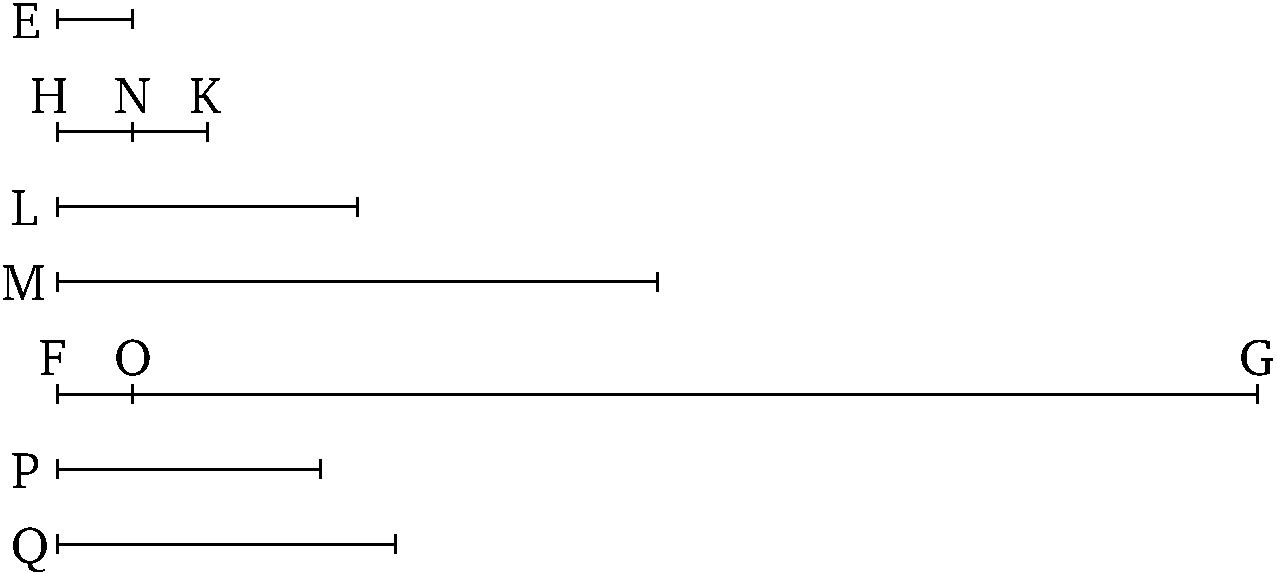
\includegraphics{Book09/fig36ae.pdf}}

For as many as is the multitude of $A$, $B$, $C$, $D$, let so many (numbers), $E$, $HK$, $L$, $M$, be taken in a double
proportion, (starting) from $E$. Thus, via equality, as $A$ is to $D$, so
$E$ (is) to $M$ [Prop.~7.14].
Thus, the (number created) from (multiplying) $E, D$ is equal to the (number
created) from (multiplying) $A$, $M$.
 And $FG$ is the
(number created) from (multiplying) $E$, $D$. Thus, $FG$ is also
the (number created) from (multiplying) $A$, $M$ [Prop.~7.19]. Thus, $A$ has made $FG$ (by) multiplying $M$. Thus, $M$ measures $FG$ according to the units in $A$.
And $A$ is a dyad. Thus, $FG$ is double $M$.  And $M$, $L$, $HK$,
$E$ are also continuously double one another. Thus, $E$, $HK$, $L$, $M$,
$FG$ are continuously proportional in a double proportion. So
let $HN$ and $FO$, each equal to the first (number) $E$, be subtracted from the second (number) $HK$ and the last $FG$ (respectively). 
Thus, as the excess of the second number is to the first, so the excess
of the last (is) to (the sum of) all  those (numbers) before it [Prop.~9.35]. Thus, as $NK$ is to $E$, so
$OG$ (is) to $M$, $L$, $KH$, $E$. And $NK$ is equal to $E$. And thus
$OG$ is equal to $M$, $L$, $HK$, $E$. And $FO$ is also equal to $E$,
and $E$ to $A$, $B$, $C$, $D$, and a unit. Thus, the whole of $FG$ is equal to
$E$, $HK$, $L$, $M$, and $A$, $B$, $C$, $D$, and a unit. And it is
measured by them. I also say that $FG$ will be measured by no other (numbers)
except $A$, $B$, $C$, $D$, $E$, $HK$, $L$, $M$, and a unit. For, if possible, let some (number) $P$ measure $FG$, and let $P$ not be the same
as any of $A$, $B$, $C$, $D$, $E$, $HK$, $L$, $M$. And as many times
as $P$ measures $FG$, so many units let there be in $Q$. Thus, $Q$ has
made $FG$ (by) multiplying $P$. But, in fact, $E$ has  also made $FG$
(by) multiplying $D$. Thus, as $E$ is to $Q$, so $P$ (is) to $D$
[Prop.~7.19]. And since $A$, $B$, $C$, $D$
are continually proportional, (starting) from a unit, $D$ will thus not be measured
by any other numbers except $A$, $B$, $C$ [Prop.~9.13]. And $P$ was assumed not (to be) the same as any of $A$, $B$, $C$. Thus, $P$ does not measure $D$. But, as $P$ (is) to
$D$, so $E$ (is) to $Q$. Thus, $E$ does not measure $Q$ either
 [Def.~7.20]. And $E$ is a prime (number).
And every prime number [is] prime to every  (number) which it does not
measure [Prop.~7.29]. Thus, $E$ and $Q$ are
prime to one another. And  (numbers) prime (to one another are) also the least (of those
numbers having the same ratio as them) [Prop.~7.21],
and the least (numbers) measure those (numbers) having the same ratio as them an equal number of times, the leading (measuring) the leading, and the
following the following [Prop.~7.20].
And as $E$ is to $Q$, (so) $P$ (is) to $D$. Thus, $E$ measures $P$ the same number of times as $Q$ (measures) $D$. And $D$ is not measured by any
other (numbers) except $A$, $B$, $C$.  Thus, $Q$ is the same as one
of $A$, $B$, $C$. Let it be the same as $B$. And as many as is the
multitude of $B$, $C$, $D$, let so many (of the set out numbers) be taken, (starting) from $E$, 
(namely) $E$, $HK$, $L$. And $E$, $HK$, $L$ are in the same ratio as
$B$, $C$, $D$. Thus, via equality, as $B$ (is) to $D$, (so) $E$ (is) to $L$
[Prop.~7.14]. Thus, the (number created) from
(multiplying) $B$, $L$ is equal to the (number created) from multiplying
$D$, $E$ [Prop.~7.19]. But, the (number created)
from (multiplying) $D$, $E$ is equal to the (number created) from (multiplying)
$Q$, $P$. Thus, the (number created) from (multiplying) $Q$, $P$
is equal to the (number created) from (multiplying) $B$, $L$. Thus, as
$Q$ is to $B$, (so) $L$ (is) to $P$ [Prop.~7.19]. 
And $Q$ is the same as $B$. Thus, $L$ is also the same as $P$. The
very thing (is) impossible. For $P$ was assumed not (to be) the same
as any of the (numbers) set out. Thus, $FG$ cannot be measured by any number except $A$, $B$, $C$, $D$, $E$, $HK$, $L$, $M$, and a unit.
And $FG$ was shown (to be) equal to (the sum of) $A$, $B$, $C$, $D$, $E$, $HK$,
$L$, $M$, and a unit. And a perfect number is one which is equal to (the sum of) its own
parts [Def.~7.22]. Thus, $FG$ is a perfect (number).
(Which is) the very thing it was required to show.}
\end{Parallel}
{\footnotesize\noindent$^\dag$ This proposition demonstrates that perfect
numbers take the form $2^{n-1}\,(2^n-1)$ provided that $2^n-1$ is a prime
number. The ancient Greeks knew of four perfect numbers: 6, 28, 496, and
8128, which correspond to $n= 2$, 3, 5, and 7, respectively.}
